%Copyright FG Mauthe, University of Koblenz-Landau, Koblenz, Germany
% v1.0, last changed 19.04.21

\documentclass[%
	BCOR=8mm, % Bindekorrektur
	DIV=12,
	toc=bibliography, % references in contents
	toc=listof, % list of tables and figures in contents
	oneside, %use twoside if preferred
	egregdoesnotlikesansseriftitles, % deletes the usage of sffamily font
	]{scrbook}

% Set the font right away, this is global, egregdoesnotlikesansseriftitles is already set, but overwritten with this command
\renewcommand{\familydefault}{\sfdefault} % bfseries

% Alternative, needs to be adjusted
%\documentclass[a4paper, twoside]{article}

%\newlength{\laenge}
%\setlength{\laenge}{2mm}
%\setlength{\parindent}{2\laenge}

\usepackage{xcolor}
\pagecolor{white} % white pages

% Font / Formatting packages
\usepackage[latin1]{inputenc}   % font-coding
\usepackage{listingsutf8}
\usepackage{caption}
\usepackage{subfigure}
\usepackage{parskip}
%\usepackage{cite}
\usepackage{lmodern}
\usepackage{multirow}
% Use either English or German
\usepackage[english]{babel}
%\usepackage[ngerman]{babel}

% Math packages
\usepackage{amsmath} % math package
\usepackage{amsfonts} % for additional mathematical symbols
\usepackage{dsfont} % double stroke fonts, for instance to depict the natural numbers symbol |N

% More useful packages
\usepackage{float} % for "containers"
\usepackage{url}
\usepackage[onehalfspacing]{setspace} % simple option to change the spacing
\usepackage{layout}
\usepackage{fancyhdr}	% header
\usepackage{graphicx}
\usepackage{booktabs} % For prettier tables
\usepackage{chngcntr} % enables the additional numbering of figures and tables
\usepackage{hyperref} % for clickable and marked cross references
%\usepackage{pdfpages}
\usepackage{forest}
\usepackage{algorithm}
\usepackage{algorithmic}


\usepackage[
backend=biber,
style=numeric-comp,
]{biblatex}

\addbibresource{references.bib}


% APPENDIX
\usepackage[toc,page]{appendix} % in case you'd like to use an appendix

\begin{document}

% Title Page
% Copyright FG Mauthe, University of Koblenz-Landau, Koblenz, Germany
% Apply the necessary changes to make this page your own

\begin{titlepage}
	
\includegraphics[height=35pt]{img/uni-logo.png}
	\hfill
	
\includegraphics[height=35pt]{img/iwvi.jpg}

	\begin{center}
	\vspace{2.5cm}	
	
	\huge\textbf{Assessment of Mean Teacher and Prominent Adversarial Unlabeled Data for Language Classification}
	
	%\vspace{2cm}


	\normalsize
	\vspace{1.5cm}	

	\textsc{\Large Masterarbeit}\\Master of Science (M.Sc.) im Web and Data Science\\[2cm] 
		
	vorgelegt von\\
	
	\textbf{\Large Bhupender Kumar Saini}\\ $ [ $219 100 887$ ] $\\ [1.5cm] 
	
	Koblenz, im February 2022
	\end{center}
	\vfill
	\begin{tabular}{ll}
		Erstgutachter: & Prof. Dr. Andreas Mauthe\\ 
		 & \small{(Institut f\"ur Wirtschafts- und Verwaltungsinformatik, FG Mauthe)}\\
		Zweitgutachter: & Alexander Rosenbaum, M. Sc. \\ 
		& \small{(Institut f\"ur Wirtschafts- und Verwaltungsinformatik, FG Mauthe)}\\
		%Ggf. ext. Betreuer eintragen.
		%Betreuer:  & Max Mustermann, M.Sc.
	\end{tabular}
\end{titlepage}


% Student's declaration
% Copyright FG Mauthe, University of Koblenz-Landau, Koblenz, Germany

% Declaration
% ===> Do NOT CHANGE anything here

\pagestyle{empty}
\begin{quote}
	\textbf{\Large Eidesstattliche Erkl\"arung}

	Ich versichere, dass ich die vorliegende Arbeit selbst\"andig verfasst
	und keine anderen als die angegebenen Quellen und Hilfsmittel benutzt habe
	und dass die Arbeit 
	in gleicher oder \"ahnlicher Form noch keiner anderen Pr\"ufungsbeh\"orde
	vorgelegen hat und von dieser als Teil einer Pr\"ufungsleistung
	angenommen wurde. 
	\\[10mm]

	\begin{tabular}{@{}p{0.82\linewidth}@{\hspace*{2ex}}r@{\hspace*{2ex}}r}
		Mit der Einstellung der Arbeit in die Bibliothek bin ich einverstanden.
		& ja $\square$ & nein $\square$ \\[1em] 
		Der Ver\"offentlichung dieser Arbeit im Internet stimme ich zu.
		& ja $\square$ & nein $\square$ \\
	\end{tabular}
	\\[20mm]


	\dotfill
	\\(Ort, Datum) \hspace{8.5cm} (Unterschrift)
\end{quote}


% Abstract in German and English language
% According to the HPA (examination office) you are obligated to write
% an abstract in English and German

\pagestyle{plain}
\pagenumbering{Roman}


% Acknowledgement EN
\begin{quote}
	\textbf{\Large Acknowledgement}\\\\
Language models has shown state-of-the-art performances in various natural language  processing task. Recent research has shown their weakness against adversarial attacks, where imperceptible noise in text can lead model to behave unexpectedly and severely degraded their performance under attack. Furthermore, the research towards defensive mechanism is comparatively less studied topic than generating prominent adversarial attacks. In this master thesis, a semi-supervised approach of fine-tuning is proposed which can lead to robust language model without compromising with original accuracy. An experiment was conducted to compare the performance of model fine-tuned using conventional method and proposed method. The experiment was performed using BERT and DistilBERT language models on two datasets.  As per experiment, the proposed approach demonstrated 0-2\% and  20-30\%  improvement in original accuracy and  accuracy under attacks over conventional method, respectively.

\end{quote}

% According to the HPA (examination office) you are obligated to write
% an abstract in English and German

\pagestyle{plain}
\pagenumbering{Roman}

% Abstract DE
\begin{quote}
\textbf{\Large Zusammenfassung}\\\\
Sprachmodelle haben bei verschiedenen Aufgaben der natürlichen Sprachverarbeitung Spitzenleistungen gezeigt. Die Forschung hat gezeigt, dass ihre Modelle anfällig für feindliche Angriffe sind, bei denen unmerkliches Rauschen im Text ihre Leistung unerwartet beeinträchtigen kann. Darüber hinaus ist die Erforschung von Verteidigungsmechanismen ein vergleichsweise weniger erforschtes Thema als die Generierung prominenter Angriffe. In dieser Masterarbeit wird ein halbüberwachter Ansatz zur Feinabstimmung vorgeschlagen, der zu einem robusten Sprachmodell führen kann, ohne die ursprüngliche Genauigkeit zu beeinträchtigen. Es wurde ein Experiment durchgeführt, um die Leistung eines Modells zu vergleichen, das mit herkömmlichen und vorgeschlagenen Methoden feinabgestimmt wurde. Dieser Bericht trägt auch dazu bei, den Umfang von Verbesserungen bei Sprachmodellen aufzuzeigen. Das Experiment wurde mit den Sprachmodellen BERT und DistilBERT an zwei Datensätzen durchgeführt. Das Experiment ergab, dass die mit dem vorgeschlagenen Ansatz feinabgestimmten Modelle eine Verbesserung von 0$\sim$2\% bzw. 20$\sim$30\% bei der ursprünglichen Genauigkeit und der Genauigkeit unter Angriffen gegenüber dem konventionellen Ansatz aufweisen. 

\end{quote}

\newpage

% Abstract EN
\begin{quote}
	\textbf{\Large Abstract}\\\\
    Language models have shown state-of-the-art performances in various natural language processing tasks. Research has shown that language models are vulnerable to adversarial attacks, where imperceptible noise in the text can degrade their performance unexpectedly. Furthermore, research into defensive mechanisms is a comparatively less studied topic than generating prominent adversarial attacks. In this master thesis, a semi-supervised approach to fine-tuning is proposed which can lead to a robust language model without compromising original accuracy. An experiment was conducted to compare the performance of a model that is fine-tuned using conventional and proposed methods. This report also contributes to revealing the scope of improvements in language models. The experiment was conducted using BERT and DistilBERT language models on two datasets. As per the experiment, the models fine-tuned by the proposed approach shows  0$\sim$2\% and  20$\sim$30\% improvement in original accuracy and accuracy under attacks over conventional approach, respectively. 
%Language models have shown state-of-the-art performances in various natural language  processing tasks. Recent research have shown their weaknesses against adversarial attacks, where imperceptible noise in text can sabotage models to behave unexpectedly and can severely degrade their performance under attacks. Furthermore, the research towards defensive mechanism is comparatively less studied topic than generating prominent adversarial attacks. In this master thesis, a semi-supervised approach of fine-tuning is proposed which can lead to robust language model without compromising with original accuracy. An experiment was conducted to compare the performance of model  that is fine-tuned using conventional and proposed method. This report also contribute in revealing the scope of improvements in language models.
%The experiment was conducted using BERT and DistilBERT language models on two datasets.  As per the experiment, the models fine-tuned by the proposed approach shows   improvement in original accuracy and accuracy under attacks over the conventional approach, respectively.  As per experiment, the models fine-tuned by proposed approach shows  improvement in original accuracy and  accuracy under attacks over conventional approach, respectively. 

\end{quote}



% Lists
\tableofcontents
\listoffigures
\listoftables

% Glossary, if necessary
% % Glossary if you want to add one, change to "Glossary" for English translation

\addchap[Abk\"urzungsverzeichnis]{Abk\"urzungsverzeichnis} 
\renewcommand{\arraystretch}{1.5} 
IWVI \dotfill Institut f\"ur Wirtschafts- und Verwaltungsinformatik\\
\renewcommand{\arraystretch}{1} 

%\cleardoubleemptypage
\newpage


% depicts chapter name, its number and page number in the heading of a page
\pagestyle{headings}
% Start page count here
\pagenumbering{arabic}
% change caption ident
\setcapindent{0pt}


%===INTRODUCTION%

\chapter{Introduction}
%The machine learning model has proven their advantages in dealing human-specific task and has been widely adopted in the every domain such as autonomous driving, healthcare, banking, manufacturing, logistics, and many more. Furthermore, machine learning model has out performed human capabilities in performing tasks  like chess, alpha Go, prediction trends and many more resulted in trend of increasing popularity and dependencies on machine learning model. Especially,
The Deep Neural Network (DNN) is widely  adopted technology in real world applications and the most studied topic as well. Its capability of solving complex problems, either linearly or non-linearly, and ease of computation gives it a advantage to other machine learning algorithms \cite{huq_adversarial_2020}. In Natural Language Processing (NLP), recent advancement in DNN  language models  has led to state-of-the-art transformer-based models like BERT,  DistilBERT, Roberta etc. \cite{devlin_bert_2019-1,liu_roberta_2019-1,sanh_distilbert_2020,lan_albert_2020}, which has outperformed in wide range of NLP tasks  and is consequently the most widely adopted models now a days.\\
But, studies have also revealed the weakness in DNN models against adversarial attacks \cite{szegedy_intriguing_2014,yuan_adversarial_2018,akhtar_threat_2018,huq_adversarial_2020,zhang_adversarial_2019} which can negatively impact its value and raised concern of trust, safety, and security. Szegedy et al. \cite{szegedy_intriguing_2014} first revealed this vulnerability in computer vision domain. Their study demonstrated that imperceptibly small perturbations in the input image can fool deep neural networks with high probability which they referred  as \textit{Adversarial Samples}. Attacks that sabotage a machine learning model with these examples are called \textit{Adversarial attacks} \cite{nicolae_adversarial_2019}. And, this study has drawn substantial attention from research community in all domains. \\
The presence of adversarial attack in text-domain was first confirmed in the study presented by Papernot et al. \cite{papernot_crafting_2016}. Their  study has shown  a small word level change in sentence structure can sabotage the DNN models. Later, various studies were published detailing different techniques to craft adversarial text samples which are comparatively higher than defensive mechanism. \\
Furthermore,  recent works also revealed that performance of language models suffers severely under adversarial attacks \cite{li_bert-attack_2020,garg_bae_2020,moradi_evaluating_2021}. Jin et al. \cite{jin_is_2020}  who proposed an approach of creating adversarial samples and proved that BERT accuracy drastically drops to less than 10\% under adversarial attacks and a pictorial example of attack can be seen in figure \ref{diag:ExampleAdversarial}. These studies raised concerns on conventional way of fine-tuning language models which is not sufficient when robustness is concerned. At the same time, it opens a scope of work towards robustness enhancement of language models.\\
The topic of adversarial attacks are extensively studied in computer vision domain than that of NLP \cite{wang_towards_2021}. And, in text domain, the focus is more on approaches related to create adversarial samples than defense mechanism. The reason being, the generation of adversarial samples in text domain are comparatively more challenging due to their discrete nature and requirement for maintaining the semantic \cite{li_bert-attack_2020}. Furthermore, there are few studies that aim at improving the robustness of language model and mostly revolves around gradient-based methods \cite{zhu_at-bert_2021,miyato_adversarial_2017,jiang_smart_2020-1}, which may be inspired by seeing its effectiveness in computer vision domain.\\
\begin{figure}[H]
    \centering
    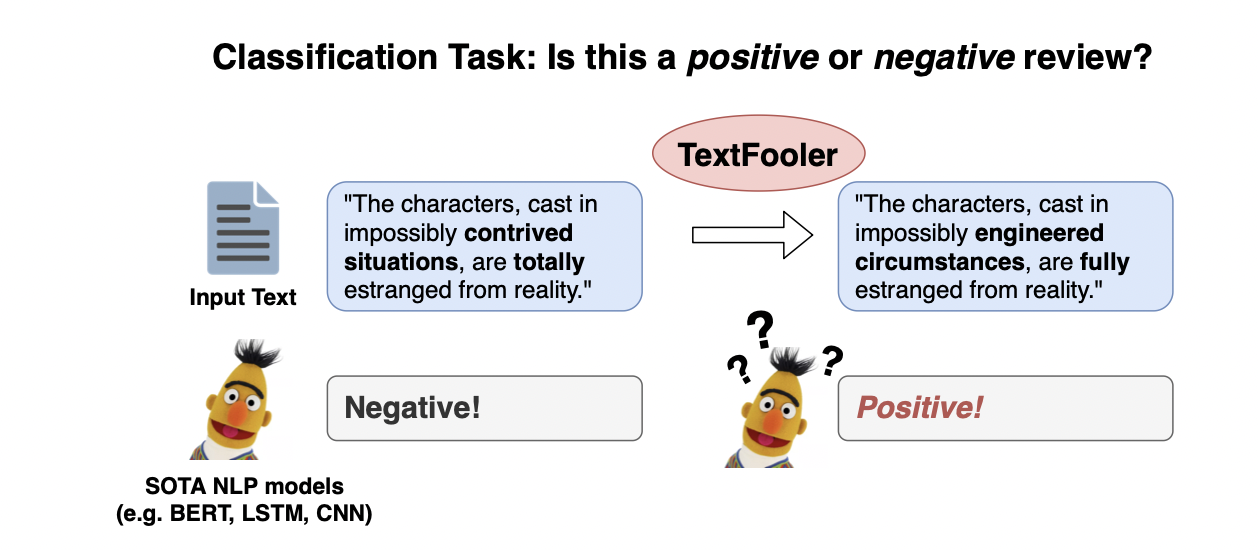
\includegraphics[width=.90\textwidth]{img/Introduction-Fig-1.png}
    \caption[Example of Adversarial attack in text-domain]{Adversarial attack presented by TextFooler \cite{jin_is_2020}, where word level changes in input text influenced the prediction.}
    \label{diag:ExampleAdversarial}
\end{figure}

Furthermore, most of the text classification tasks such as fake news detection suffers from a lack of labeled data in comparison to unlabeled data. A number of semi-supervised training approaches have been proposed to overcome these challenges, and these semi-supervised training have shown significant improvements in performance. As an example of a semi-supervised approach, mean teacher \cite{tarvainen_mean_2018}  has performed well in image-domain, however its efficiency in text domain especially with language models hasn't been examined. Implementing such a technique would be quite a challenge because different noise strategies and training approaches are needed to leverage such an approach. In another study, Belinkov et al. \cite{belinkov_synthetic_2018} showcased that including noisy data in training samples may result in robust models. Until now, no relevant study has been conducted on the  semi-supervised fine-tuning of language models and robustness evaluation as well. \\
Therefore, this master thesis study proposes a semi-supervised way of fine-tuning language models that can lead to a comparatively robust model without compromising in original accuracy. As a next step, a quantitative experiment is conducted to compare the performance of proposed approach with the conventional approach of fine-tuning. Additionally, language model capabilities such as back translation and context rewriting to generate prominent adversarial unlabeled samples are also utilized for training purpose. The main focus of the study is to answer the research hypothesis i.e. the proposed fine-tuning method will provide a comparatively better model for text classification in terms of generalization and robustness.\\
The proposed study also contributes in observing performance of the language models under worse conditions so mitigation strategies can be planned. To increase DNN's robustness, it's vital to understand how adversarial attack recipes work and how to protect against them. Moreover, also demonstrate the scope of improvements. The robustness assessment is achieved by observing the model's performance against four attack recipes and various metrics. Furthermore, this study also discusses the brief background about of text representation evolution, working of language models, and adversarial attacks. 
%The outline of the report starts with a brief background information about the relevant topics i.e. evolution of text representation from TF-IDF to contextualized embeddings, transformer based language models, and the BERT/DistilBERT  models architecture. Next, we discuss the background and classification of adversarial attacks. After that, a detailed explanation of the proposed approach and attack recipes follows. Details about the experiment environment, and the results are discussed in the experiment chapter. The master thesis is concluded by addressing limitations, challenges, and the final conclusion.

%\textit{ Different researchers worked tirelessly and showed that DNN models were vulnerable in object recognition systems (Goodfellow et al., 2014), audio recognition(Carlini and Wagner, 2018),
%    malware detection (Grosse et al., 2017), and sentiment analysis systems (Ebrahimi et al., 2017) as well. An example of the adversarial attacks is shown.\cite{huq_adversarial_2020}
%    In the field of NLP, Papernot (2016) paved the way by showing that adversarial attacks can be implemented for textual data as well. \cite{huq_adversarial_2020}}
%In real life, people are increasingly inclined to search for related comments before shopping, eating or watching film and the corresponding items with recommendation score will be
%given at the same time. The higher the score is, the more likely it is to be accepted by humans. These recommendation apps mainly take advantage of sentiment analysis with others previous
% comments . Thus attackers could generate adversarial examples based on natural comments to smear competitors (see Fig.1.1 for instance) or do malicious recommendations for shoddy
% goods with the purpose of profit or other malicious intents. Apart from mentioned above, adversarial examples can also poison network environment and hinder detection of malicious
% information [21], [22], [23]. Hence, it is significant to know how adversarial attacks conduct and what measures can defend against them to make DNNs more robust."A survey on Adversarial Attacks and Defenses in Text" Unfortunately, studies that address the defense mechanisms and robustness of the model are few and generally revolve around gradient-based training. Moreover, few studies deal with adversarial
%training of BERT \cite{zhu_at-bert_2021,du_adversarial_2020}.

%TODO:
%What are the research question ? \\
%\textbf{Research Questions}:
%\begin{enumerate}
%    \item How does BERT model works and understanding the Transformer architecture?
%    \item Empirical study of performance proposed model and BERT model in terms of efficacy in absence of adversarial attacks.
%    \item Empirical study of performance of proposed model and BERT model under adversarial attacks.
%\end{enumerate}
% As a result of experiment, found that
% Evaluated with what and dataset details ?\\
% BERT attacking BERT, PWWS, TextBugger, Textfooler.\\
% Evaluation Results\\
% short conclusion\\

 %%%%%%%%%%%%%%%%%%%%%%%%%%%%%%%%%%%%%%%%%%%%CHAPTER BACKGROUND%%%%%%%%%%%%%%%%%%%%%%%%%%%%%%%%%%%%%%%%%%%%%%%%%%%%%
\chapter{Background}
\label{section:background}
This chapter discusses about the contents required to understand the experiment and motivations behind this master thesis. We begin with a discussion of advancement in text representations, followed by a discussion of transformers architecture, one of the main principle of recent contextualized embedding. Later, fine-tuning of the language model is carried out. An overview of adversarial attacks is provided at the end of  section. If the reader already has a basic understanding of the topic, it is recommended to skip this chapter.
\section{Text Representations (2 pages)}
\label{section: textrep}
In natural language processing, researchers explore how a computerized system can understand and manipulate natural language (speech or text) to perform various tasks\cite{chowdhury_natural_2003} and aims to gain human-level understanding of the text \cite{naseem_comprehensive_2020}. However, there was a major challenge in converting text into numbers or vectors in such a manner that semantic and syntactic information can be retrained. As shown in figure \ref{fig:onehot}, traditionally words were usually represented as a single hot vector in a discrete manner, where each word is shown as a vector of 1 and 0 \cite{salton_vector_1975}. The shape of vector is equal to the size of vocabulary which suffers from dimensionality curse and also lacks semantic relationship between words. Later, researchers developed low-dimensional and continuous vector representations of text and discovered word embedding.
\begin{figure}[h!]
    \centering
    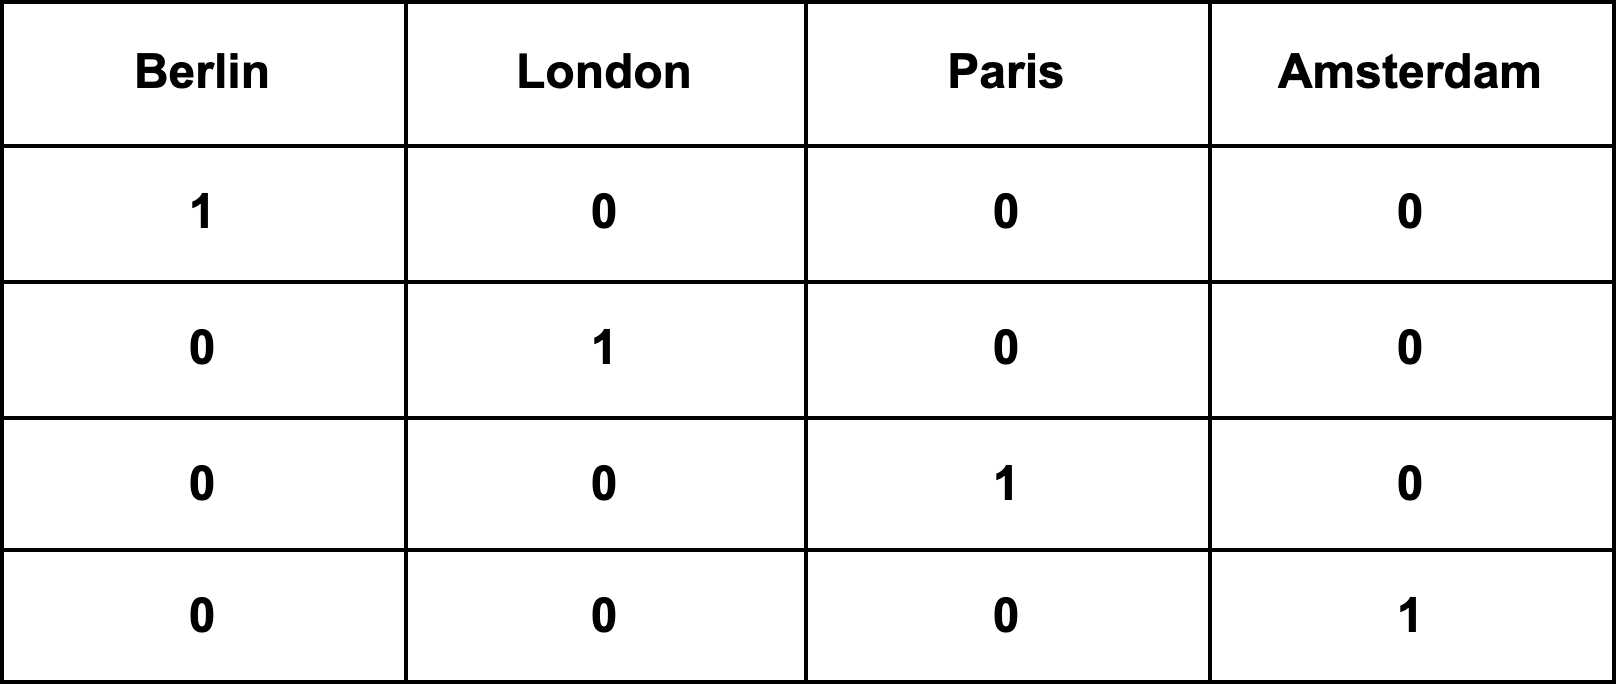
\includegraphics[width=0.4\linewidth]{img/onehot.png}
    \caption[Example of one hot encoding.]{ An example of one hot encoding, the dimension of vector increases with vocabulary size.}
    \label{fig:onehot}
\end{figure}
\subsection{Word Embeddings}
\label{subsection:wordembeddings}
Vector representations that map the words and phrases to numbers in a real world vector are called  word embeddings \cite{almeida_word_2019-1}. The distributed hypothesis is the main principle behind this type of representations \cite{harris_distributional_1954}, which posits that the words of similar contexts tend to have same meanings. This type of word embedding can be utilized to perform various NLP tasks. Mikolov et al. \cite{mikolov_efficient_2013} proposed Word2Vec , ``a continuous vector representation of words from very large datasets'', where a CBOW (continuous bag of words model) and skip-gram model architectures are utilized to learn the representation. The goal of CBOW is to predict the middle word when given past and future words as inputs. At the projection layer, each word's context is averaged as shown in figure 2.2. As order of the words does not influence projection of the word hence called bag-of-words. \\
Word2Vec also uses skip-gram to maximize classification of a word based on another word in the  sentence, as shown in figure 2.2.  There are two major concern with Word2Vec i.e. (1) It only preserves the local information of words,  and (2) The semantics of a given word is entirely determined by the surrounding words.

\begin{figure}[h!]
    \centering
    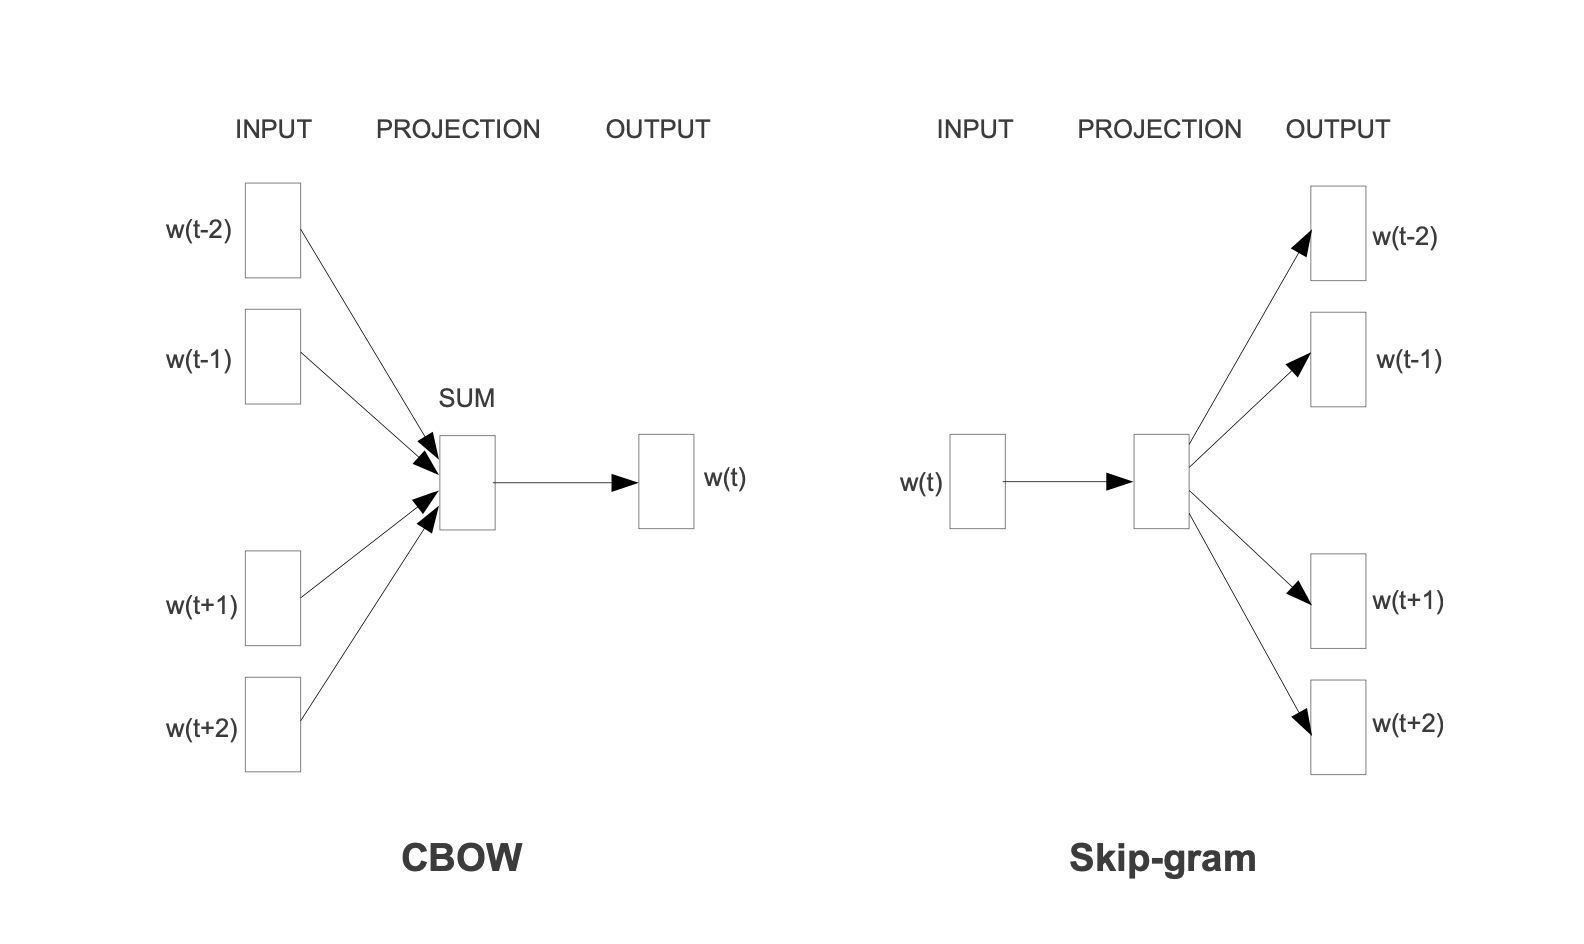
\includegraphics[width=0.7\linewidth]{img/cbowandskip.png}
    \caption[Working diagram of CBOW and skip-gram models]{ The CBOW architecture predicts the current word given past and future words, and the skip-gram architecture predicts the surrounding words given the current words.}
    \label{fig:cbow}
\end{figure}
Later, Penning et al. \cite{pennington_glove_2014} proposed word embedding called Glove (Global Vectors for Word Representation) which was based on word global information and a big corpus of unlabeled datasets. The idea is to determine how frequently a word pair occurs together by using a co-occurrence matrix and factorize it into a lower dimensional space to reduce reconstruction loss. The approach was mainly based on global matrix factorization and local context window methods such as skip-gram, which led to log-bilinear regression model where the probability of next word is determined by the previous word.\\
 Both, Word2Vec and Glove word embeddings are static and have a limitation called polysemy, which refers to the fact that meaning of a word differs across contexts. For example, based on the context, ``jaguar'' might refer to an animal or to a car brand. These traditional approaches missed these deep details, and provided a direction of working on contextualized word embeddings.

 \subsection{Contextualized Embeddings}
 \label{subsection:contextembeddings}
 Matthew, et al.\cite{peters_deep_2018-3} proposed the ELMO(Embedding from Language Model) as methods to create context-sensitive embedding. The ELMO model uses a bi-directional LSTM to extract contextualized word features to address the problem of polysemy. The model is further optimized by next word prediction using a large corpus of data. A layer's weight can later be used as contextual embedding. \\
 Later, after transformer architecture introduced by  Vaswani et al. \cite{vaswani_attention_2017}, Generative Pre-training (GPT) \cite{radford_improving_nodate}, and Bidirectional Encoder Representation From Transformers (BERT) \cite{devlin_bert_2019-1} utilized  encoders or decoders instead of bidirectional LSTMs to create contextualized embedding. GPT uses decoder architecture where as BERT uses encoder architecture, however, the main concept of is based on ELMO, as shown in figure \ref{fig:elmo}. \\
 Both of these approaches introduce the concept of \textit{pre-training}, i.e. learning embedding using large corpora of unlabeled data, and \textit{fine-tuning}, i.e. optimizing weights further based on downstream task. Furthermore, also the approach of transfer learning can be utilized in NLP to get the state-of-the-art performance. A brief overview of the transformer model is required to understand language models work, so the next section discusses the transformer before language models.

\begin{figure}[h!]
    \centering
    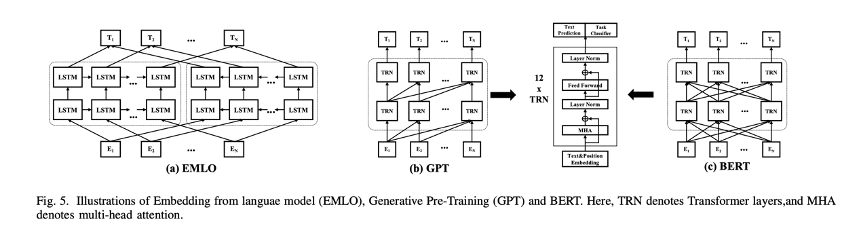
\includegraphics[width=1.0\linewidth]{img/elmo}
    \caption{Different Contextualized Embeddings model.}{Pictorial representation of working of (1) ELMO(Embedding from language model),  (2)Generative Pre-training (GPT), and (3) Bidirectional Encoder Representation From Transformers(BERT). TRN represents transformer encoder in BERT and decoder in GPT.}
    \label{fig:elmo}
\end{figure}

\section{Transformers}
\label{section: transformers}
There was a time when NLP tasks were solely based on sequential models like CNN, RNN, LSTM, and BiLSTM models which had the disadvantage of being computationally expensive, lacking distributing capabilities, and having only satisfactory performance. In order to reduce the amount of sequential computation,  Vaswani et al. \cite{vaswani_attention_2017} proposed an attention based architecture called the transformer, which later outperformed the existing state-of-the-art NLP models. A transformer architecture was developed which is exclusively based on a type of attention mechanism called self-attention. Comparatively, this architecture has faster training times because of its distributed properties, and showed better evaluation results. 
Later, this transformer architecture became the one of the main principles behind the development of break-through models like BERT, GPT, and T5. Figure \ref{diag:TransformerArchitecture} illustrates the architecture of a transformer.

\begin{figure}[h!]
    \centering
    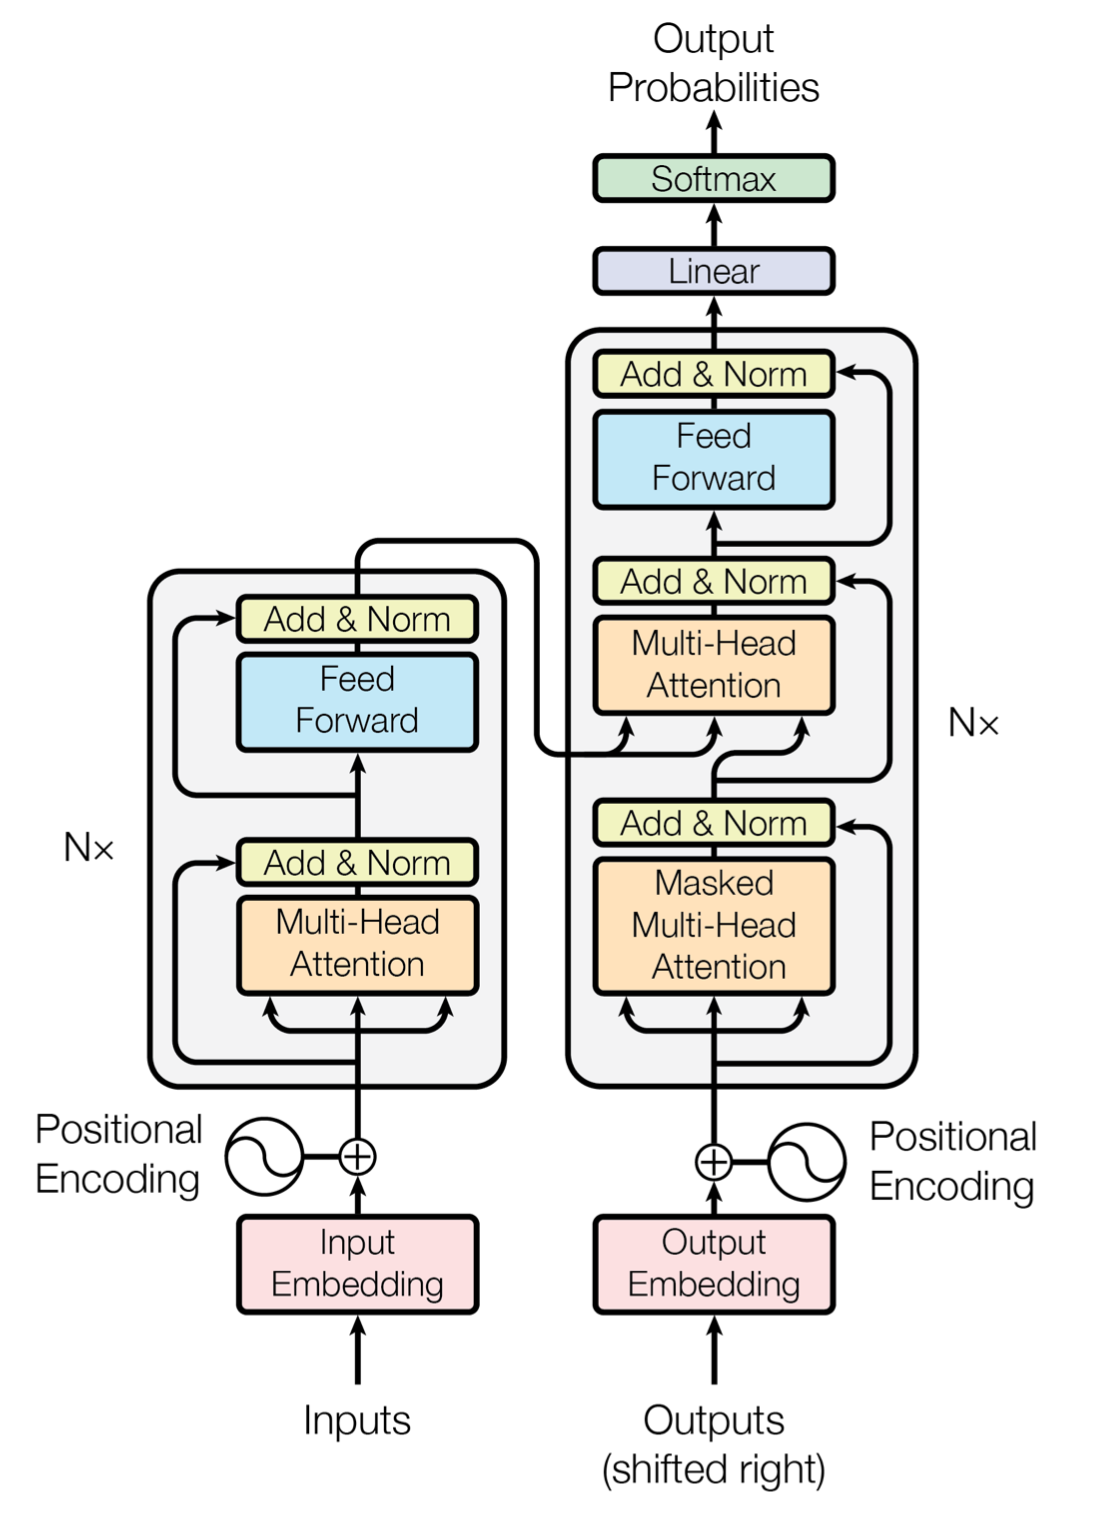
\includegraphics[width=.50\textwidth]{img/TransformerArchitecture.png}
    \caption[Architecture diagram of Transformer]{Transformer Model Architecture \cite{vaswani_attention_2017}.}
    \label{diag:TransformerArchitecture}
\end{figure}
Transformers are encoder-decoder stacks where the encoder reads inputs and outputs representation as a context vector, often referred to as a "contextualized embedding," as illustrated in figure \ref{diag:EncoderDecoder}, which is based on single or multi-headed attention, and the decoder makes predictions based on those context vectors. Vaswani et al. \cite{vaswani_attention_2017} proposed the  transformer model which consist 6 layers of encoders stacked on top of each other and same applies to decoders. Encoder is composed of multi-head attention followed by layer normalization and feed forward networks. However, there is slight difference in decoder i.e. masked multi-head attention layer is followed by multi-head attention layer as shown in figure \ref{diag:TransformerArchitecture}.

\begin{figure}[h!]
\centering
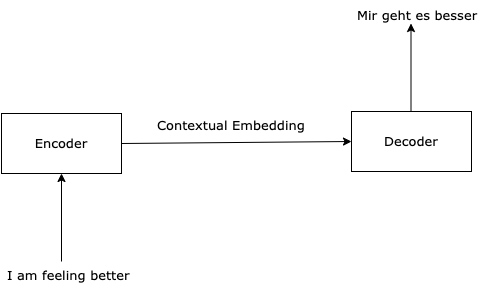
\includegraphics[width=.50\textwidth]{img/encoderDecoder.png}
\caption[Basic example of encoder and decoder]{Basic example Encoder Decoder.}
\label{diag:EncoderDecoder}
\end{figure}

\subsection{Encoder Architecture}
In machine translation, the main difficulty was to translate variable length inputs to another variable length output. As a result, encoder and decoder are proposed as solutions, where encoder learns the pattern of variable length input and generates a fixed shape output. A decoder, on the other hand, takes that fixed shape as input and gives variable length as output. \\
For example, the task is to translate english sentence ``I am good. How are you ?'' to German language , given input sequence of tokens ``I``, ``am'', ``good'',...,``?'' to encoder which generates the fixed shape representation $z_{1},z_{2},z_{3}$. Using this representation, decoder outputs the ``Mir geht es gut. Wie geht es dir ?'' in token format as shown in figure \ref{diag:EncoderDecoderExp}.\\
\begin{figure}[H]
    \centering
    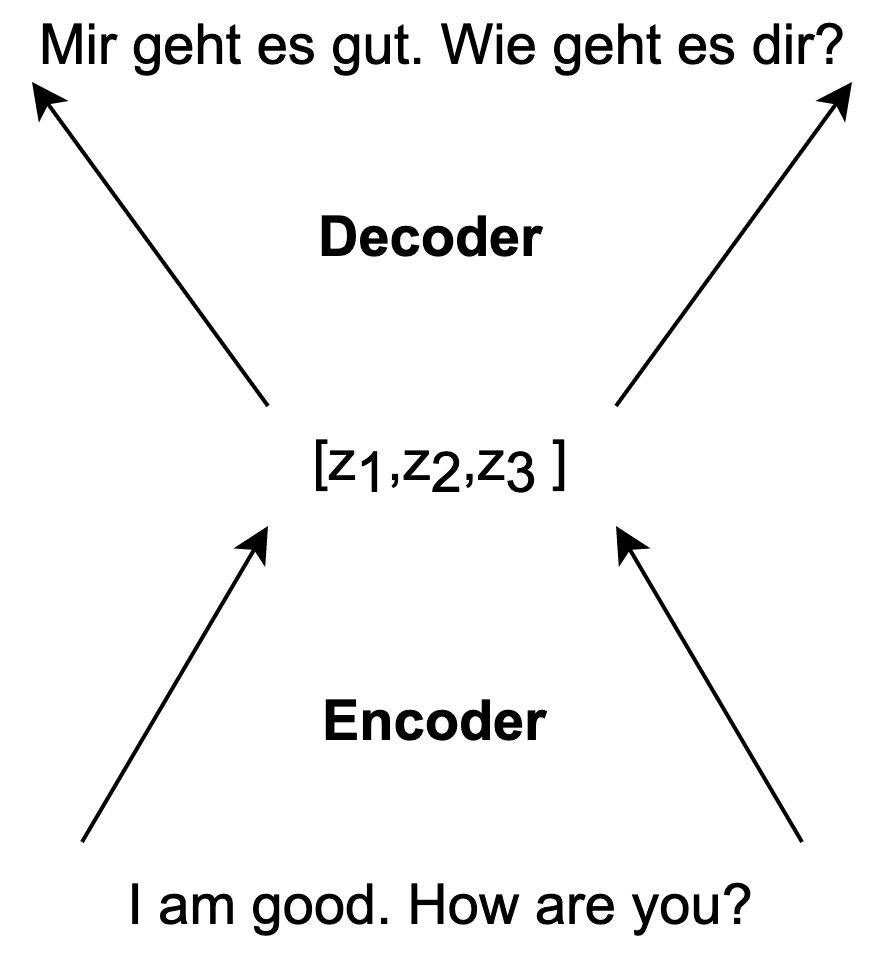
\includegraphics[width=.30\textwidth]{img/EncoderDecoder2.png}
    \caption[Basic example of encoder and decoder working]{Basic working example of encoder decoder.}
    \label{diag:EncoderDecoderExp}
\end{figure}
 Later, several sequence to sequence models utilize this encoder-decoder architecture to perform task such as text summarization, question answering, and machine translation. However, the encoder decoder architecture in transformer differs significantly.\\
A transformer encoder block is further divided into three layers as shown in figure \ref{diag:EncoderArch}: multi-head attention, normalization layer, and feed forward network. The input embedding component converts the input text tokens into embedding vectors $EM$ of shape $d_{model}$.
\begin{figure}[H]
\centering
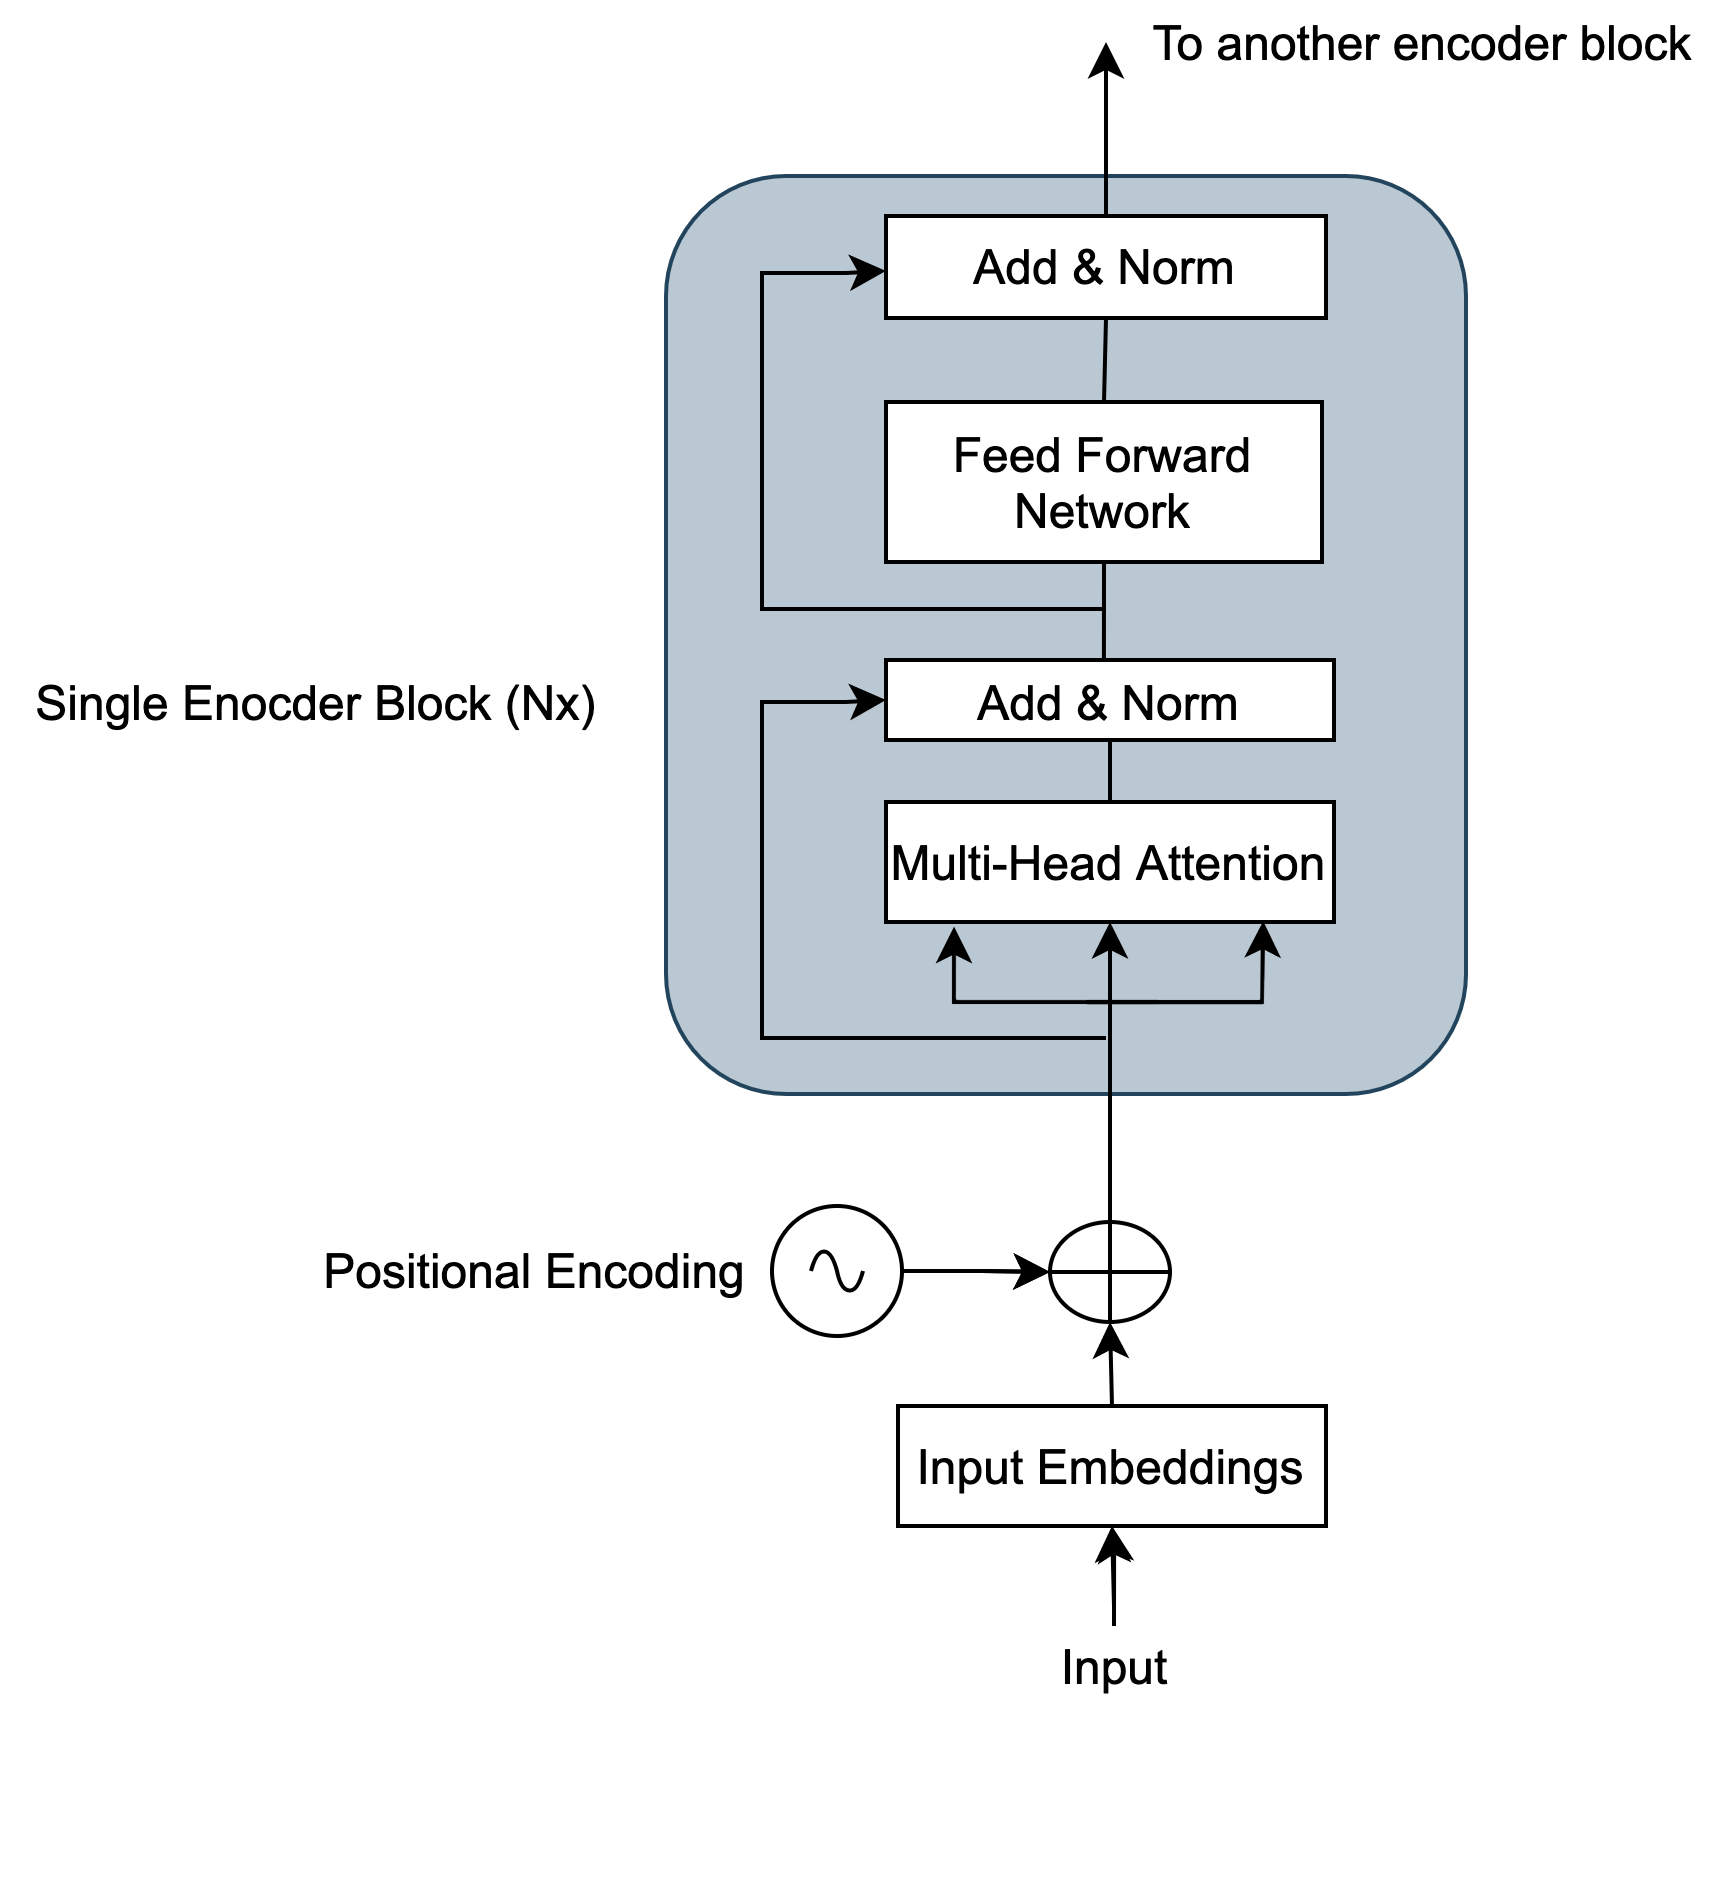
\includegraphics[width=.50\textwidth]{img/EncoderArch.png}
\caption[Different components of encoder in transformer]{Different components of encoder in transformer.}
\label{diag:EncoderArch}
\end{figure}
\subsubsection{Positional Encoding}
Sequential models understand sentences and contain information about word position, however, in transformer models, sentences are fed all at once, so a separate mechanism was introduced to determine word order. The word order in the shape of a position vector will be added to the input embedding before the multi-head attention. Position vector must have the same dimension as word embedding $d_{model}$.\\
Two major constraints that applies: First, the word embedding information should not be severe and second, word position must be identical. According to Vaswani et al. \cite{vaswani_attention_2017}, sine and cosine functions of different frequencies are used to form geometric progression from  $2\pi$ to $2\pi \cdot 10000$ used for calculating the position vector($PV$) of the words. In other words, mentioned function \ref{eq:PV} generates unique values containing information about the position of words in a sentence.
\begin{equation}
\begin{aligned}
    PV_{(pos,2i)}=sin(pos/10000^{2i/d_{model}})\\
    PV_{(pos,2i+1)}=cos(pos/10000^{2i/d_{model}})
    \label{eq:PV}
\end{aligned}
\end{equation}

Where $pos$ \& $i$ is position and dimension respectively. And, after adding to the embeddings we get position encoding ($PE$)
\begin{equation}
\begin{aligned}
    PE_{word} =EM_{word}+PV_{word}\\
    \label{eq:PE}
\end{aligned}
\end{equation}

%For, a  sentence $S$ with $n$ number of words ($w_{1},w_{2},...,w_{n}$) with embedding vector($EM$) is $e_{1},e_{2},....,e_{3}$ , positional vector ($PV$) as ($pv_{1},pv_{2},...,pv_{n}$) and positional encoding ($PE$) as ($pe_{1},pe_{2},...,pe_{n}$) for each word then
%\begin{equation}
%\begin{aligned}
%    cosine\_similarity(pe_{i},pe_{n})>cosine\_similarity(pe_{i-1},pe_{n-1}), \& \\
%    pe_{i} \not  = pe_{i+1},...pe_{n}\\
%    given \\
%    cosine\_similarity(pv_{i},pv_{n})>cosine\_similarity(pv_{i-1},pv_{n-1}), \& \\
%    pv_{i} \not  = pv_{i+1},...pv_{n}
%    \label{eq:PE_example}
%\end{aligned}
%\end{equation}
%
%For example in a sentence ``I am good. How are you?'' , the cosine similarity of positional vector of word ``I'' and ``you'' must be higher than word ``am'' and ``you'' and so on. And, same applies to positional encoding.

\subsection{Attention Mechanism}
The human mind does not process all the information available in environment, but rather, it focuses on specific information to complete the task and this biological mechanism is called attention. And, the major intention behind achieving the same in machine learning tasks. In 1964, Naradaya et al. \cite{nadaraya_estimating_1964} first introduced the idea of attention in regression model, proposing a weighted function $a(x,x_{i})$ which encodes the relevance of features. In 2015, Bhadanu et al. \cite{bahdanau_neural_2014} proposed encoder-decoders that include attention mechanisms at the decoder level. Later, Luong et al. \cite{luong_effective_2015} showed that attention mechanisms gained up to 5.0 BLEU over non-attention models in neural machine learning tasks. And, recently, Kardakis et al. \cite{kardakis_examining_2021} studied the same mechanism in the text classification task, i.e. sentiment analysis, and reported 3.5\% increase in accuracy.\\
Attention mechanism in transformer architecture model introduced to reduce computational complexity and facilitate computation \cite{vaswani_attention_2017}. Different types of methods exist to calculate attention mechanisms such as similarity based \cite{graves_neural_2014}, dot products \cite{luong_effective_2015}, scaled dot products \cite{vaswani_attention_2017}, additives \cite{bahdanau_neural_2014}, etc. This report focuses on scaled dot product attention used in transformer models. Equation  \ref{eq:selfattention}  and figure \ref{fig:selftattentionandmulti} demonstrate how to calculate the scaled dot product or self-attentions.
\begin{equation}
    \begin{aligned}
        Attention(Q,K,V)=softmax(\frac{QK^T}{\sqrt{d_{k}}})V\\
        \label{eq:selfattention}
    \end{aligned}
\end{equation}
Where $Q$, $K$, and $V$ is query, key, and value vector which is created  by dot product of different trainable weight matrix $w_{q},w_{k}$, and $ w_{v}$ with input. With this attention mechanism, the relationship between words is more profound, resulting in better performance.\\
\begin{figure}
    \centering
    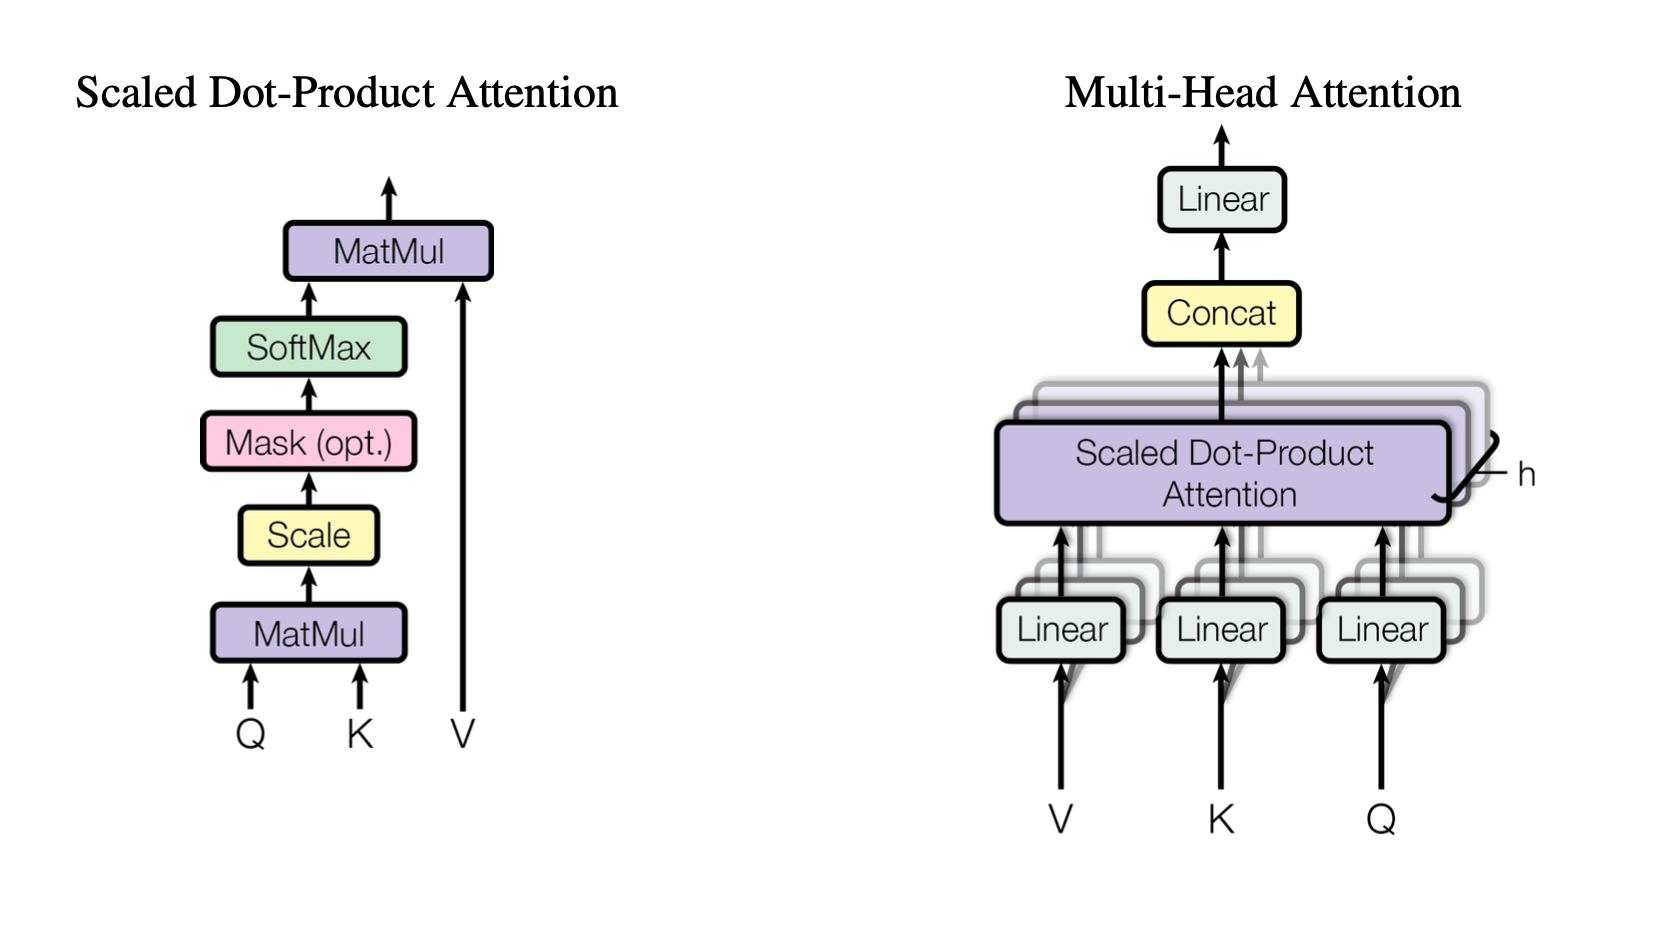
\includegraphics[width=0.7\linewidth]{screenshot001}
    \caption[Calculation flow diagram of Scaled dot product and multi-head attention]{\small Scaled dot product and multi-head attention calculation flow diagram \cite{vaswani_attention_2017}. }
    \label{fig:selftattentionandmulti}
\end{figure}
In order to capture the different perspectives of the sentence and ensure better accuracy, multiple attention heads are calculated instead of just one. Then, concatenating the result provides a comparatively better attention matrix called multi-head attention and this mechanism exploits the parallelization feature.\\
Further, the add and norm component is basically a residual connection followed by layer normalization that prevents heavy changes in values during training. Later, feed forward network consists of two dense layers activated by a ReLU. 
%In Decoder is similar to encoder attention mechanism except masked multi-head attention at the beginning of decoder, this approach prevent  to calucate attention upto current position and future words are masked ($-\infty$)  and this gives the capability of of next word prediction.
\section{Language Models}
\label{section:langaugemodels}
The language model is a function that learns the word representation from the corpus and provides vectors that can be utilized for further downstream tasks such as machine translation or sentiment analysis. A number of techniques are available to learn a representation, either statistically or by means of neural networks. In recent years, neural network-based language models, such as BERT and DistilBERT, have become the cornerstone of Natural Language Processing (NLP). 
\begin{figure}[H]
    \centering
    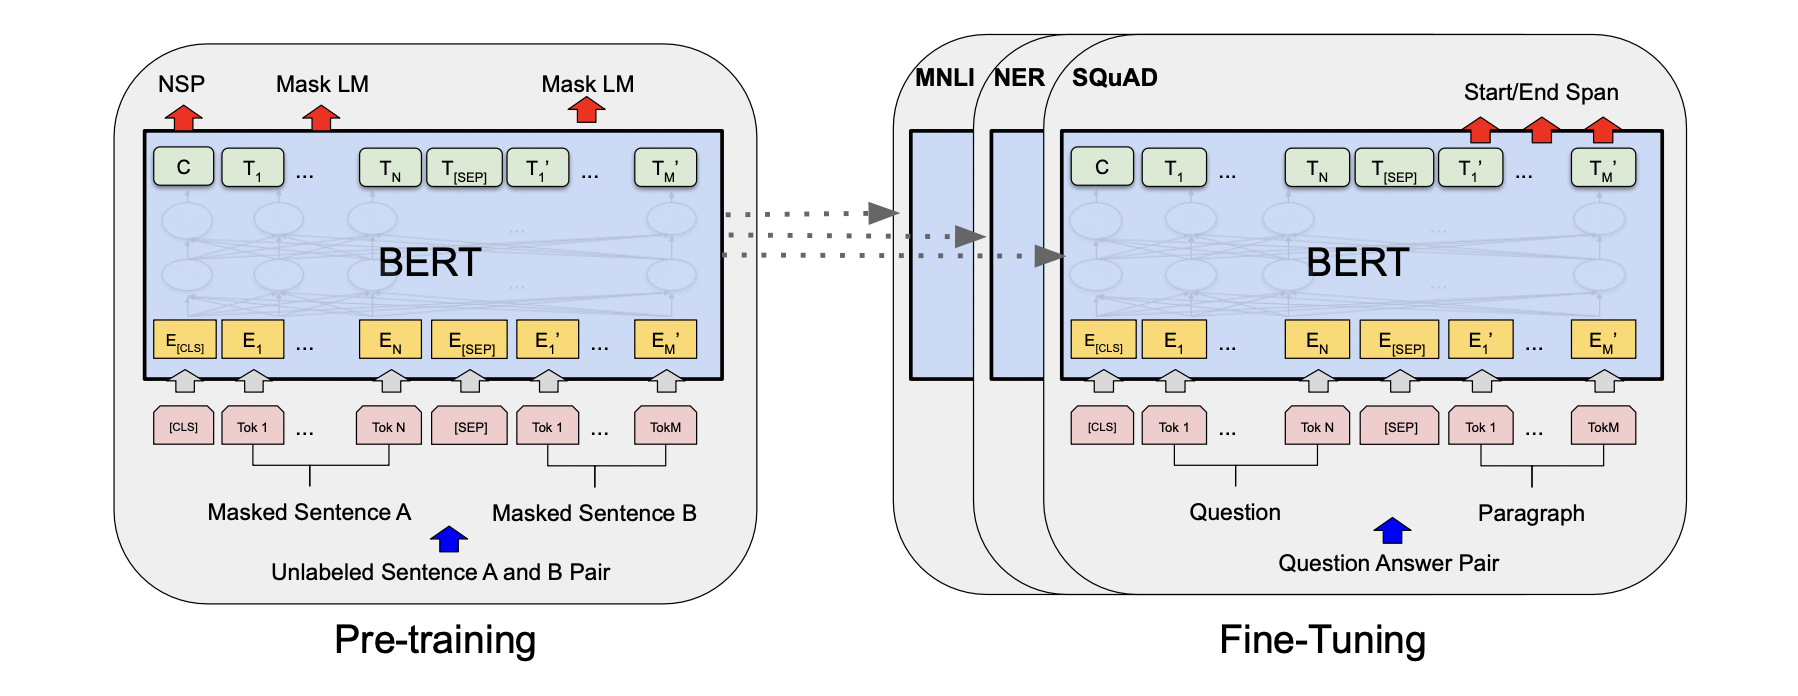
\includegraphics[width=0.7\linewidth]{img/pre_fintune.png}
    \caption[Diagram of of pre-training and fine-tuning of BERT model]{ \small Pre-training and fine-tuning method of the BERT model \cite{devlin_bert_2019-1}. In pre-training, unsupervised techniques such as next sentence prediction (NSP) and masked word prediction (MWP) are utilized. Pre-trained models are provided to perform further downstream tasks and weights are further optimized during fine-tuning.}
    \label{fig:prefintune}
\end{figure}
According to figure , these language models follow two training processes, (1)\textit{ Pre-training} by using huge unlabeled text corpora and generating a context representation vector from the model \cite{devlin_bert_2019-1}  and enables the transfer learning. The pre-training mechanisms of BERT and DistilBERT are discussed in more detail in this section. (2) \textit{Fine-tuning}, user adapts the pre-trained language model to perform specific tasks by adding a feed-forward layer on top of language models as per task and further train the weights with limited data for the target task. The fine-tuning approach can be performed in low-resource environments and have achieved state-of-the-art performance in many popular NLP benchmarks.


\subsection{BERT (Bidirectional Encoder Representation From Transformers)}
BERT (Bidirectional Encoder Representations from Transformers) was proposed by Devlin et al.\cite{devlin_bert_2019-1}, primarily based on Transformers \cite{vaswani_attention_2017}, ULMFit \cite{howard_universal_2018}, ELMo \cite{peters_deep_2018-3}, and the OpenAI transformer \cite{radford_improving_nodate}, but not limited to it. In essence, BERT is a transformer encoder stack that outputs the context representation, also called a pre-trained model. \\
BERT model is pre-trained on deep bidirectional representation of large unlabeled text in both right and left context, which can be further fine-tuned by adding additional output layers to achieve state-of-the-art results in various NLP tasks like text classification, question answering, language inference, language translation, etc. Its main benefit is simplifying the process of NLP tasks in machine learning, and providing access to contextualized embedding trained on huge amounts of words, which are impossible to collect individually. In addition, it requires high performance computational machines at production scale. \\
Having access to vast amounts of unlabelled data,  BERT uses two learning strategies: Masked Language Model (MLM) and Next Sentence Prediction (NSP). MLM replaces 15\% of words with [MASK] tokens, and BERT predicts the masked word based on other words in the sequence.\\
In NSP, BERT models are given two pairs of sentences, with [CLS] as the sentence start and [SEP] as the separation between sentences. The BERT model then predicts whether the next sentence is correct or random. The BERT model is pre-trained on a large amount of unlabeled text, however, fine-tuning is still required for specific tasks.\\
To enable BERT models to handle a variety of downstream tasks, the input representations are a sum of three different embeddings (position embeddings, segment embeddings, and token embeddings), as shown in figure \ref{fig:bert_inp}.
\begin{figure}[H]
    \centering
    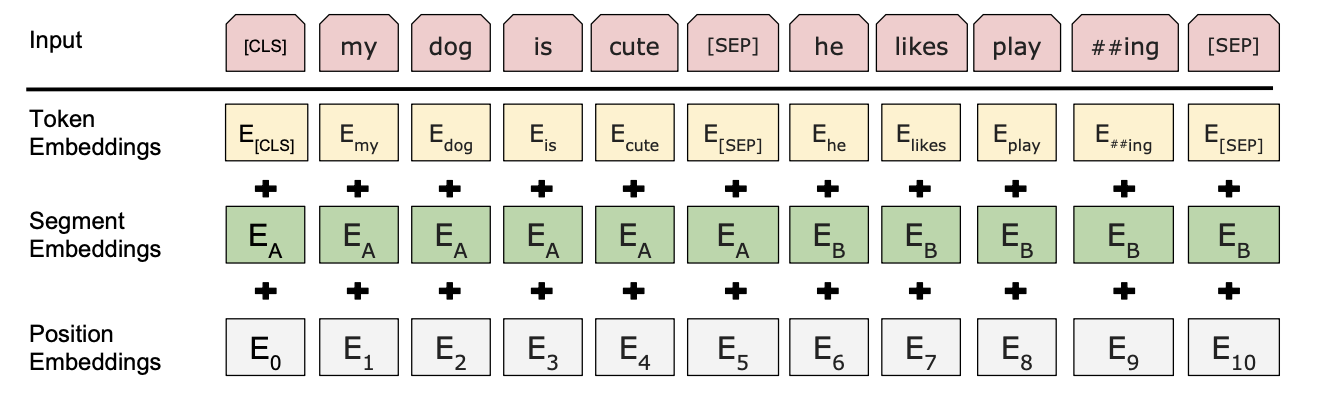
\includegraphics[width=0.6\linewidth]{img/bert_inp.png}
    \caption[Three different embeddings in BERT model]{\small BERT model input includes three different embedding information to perform various downstream task\cite{devlin_bert_2019-1}. }
    \label{fig:bert_inp}
\end{figure}
A BERT paper \cite{devlin_bert_2019-1} described two BERT models on which they conducted their experiments. 
\begin{enumerate}
    \item $BERT_{BASE}$ $:$ 12 Transformers blocks(Encoder, L), 768 Hidden Units(H), Attention Heads(A) 12, Total Parameters 110M.
    \item $BERT_{LARGE}$ $:$ 24 Transformers blocks(Encoder, L), 1024 Hidden Units(H), Attention Heads(A) 16, Total Parameters 340M.
\end{enumerate}
In this master thesis experiment, $BERT_{BASE}$ model  pre-trained on lower case words is utilized. 

\subsection{DistilBERT- A distilled version of BERT}
DistilBERT is a compact version of BERT proposed by Victor et al. \cite{sanh_distilbert_2020}. As compared to BERT, the DistilBERT model does not incorporate token embeddings, poolers, and have comparatively half hidden layers. The principle behind this model is based on knowledge distillation \cite{hinton_distilling_2015}, which can be defined as a process of transferring knowledge from large  to small models. \\
\begin{figure}[H]
    \centering
    \includegraphics[width=0.8\linewidth]{img/DistilBERT.png}
    \caption[Diagram of DistilBERT training.]{ Pictorial diagram depicts the knowledge distillation process involved in  DistilBERT.}
    \label{fig:DistilBERT}
\end{figure}
As illustrated in figure \ref{fig:DistilBERT}, a small model is trained to mimic the behavior of a larger model. In the task of mask word prediction, masked sentences are supplied to both the BERT and DistilBERT models.\\
This approach aims to minimize three losses: 1) the loss between BERT and DistilBERT predictions, 2) the loss between DistilBERT predictions and ground truth, and 3) the cosine embedding loss, which measures the distance between the representations learned by BERT and DistilBERT. Cosine embedding loss reduction makes representation more accurate and tries to copy the BERT embeddings. The proposed approach is 40\% compact, retaining 97\% of its language understanding capabilities and 60\% faster \cite{sanh_distilbert_2020} , which has proven it is possible to reduce the size of large language models with minimal compromise.



\section{Adversarial Attacks}
\label{section:advattacks}
In the year 2013, Szegedy et al. \cite{szegedy_intriguing_2014} study in the image-domain discovered that deep neural networks are vulnerable to perturbations, which can result in unexpected behaviors, referred to as adversarial attacks. It was first demonstrated by Papernot et al.  \cite{papernot_crafting_2016} that an adversarial example can also lead to an unexpected outcome in the text domain. Later various papers on different attack recipes were published in text domain \cite{alzantot_generating_2018,li_bert-attack_2020,gao_black-box_2018,li_bert-attack_2020,ren_generating_2019,garg_bae_2020,chen_robustness_2019}.  Sun et al.  \cite{sun_adv-bert_2020} proposed an approach of  generating adversarial misspelling and evaluated the performance of  attack recipes  against BERT model. Based on their experiment on Stanford Sentiment Treebank (SST) dataset, the BERT model is vulnerable to misspelling attacks and its accuracy decreases by 22.6\% under their proposed attack.\\
In another experiment, Li et al. \cite{li_bert-attack_2020}, proposed an approach of utilizing BERT model to generate word for replacements. Firstly, identifying the most important words i.e. the words in sequence have a high influence on the final output logit. Secondly, utilizing BERT model masked language model(MLM) capability to generate word for replacements. According to their claims, the accuracy under attack is lower than 10\% with less than 10\% perturbation. However, there is a possibility of compromising with semantic constraints.\\
In text domains, most adversarial attacks consist of two steps: 1) Identification of the most important word, and 2) Replacement of the word with suitable words. The reason behind why DNN models are vulnerable to attacks is still an open question. The presence of adversarial attacks in DNN models, according to Goodfellow et al. \cite{goodfellow_explaining_2015}, is due to the linearity in DNN models.

\subsection{Definition}
\label{subsection:definition}
For a given input data and its labels $(x, y)$ and a classifier F function which classify inputs x to its respective class label y i.e. $F (x) = y$. However, adversarial attack techniques introduce small perturbation $\delta$ in input data.\\
Hence, the attack would be an untargeted adversarial attack if $F(x+\delta)\not=y$ and target when $F(x+\delta)=y'$ in constraint of the perturbation $\delta$ must be imperceptible to humans which can be defined by a threshold  $||\delta||<\epsilon$. \\
Most common metrics to determine perturbation $\delta$ and define threshold $\epsilon$ are cosine similarity, euclidean distance, jaccard coefficient, and word mover distance.  However, in the text domain, it is really challenging to create adversarial example because human can easily detect a minute change in character, word or sentence level.\\
A particular classifier would be called robust against a particular adversarial example  $(x+\delta)$ if a classifier F should predict correct class $y$  i.e.  $F(x+\delta)=y$. And, various metrics to evaluate model robustness such as accuracy under attack, number of queries, word perturbation and  attack success are discussed in length at section \ref{section:metrics}.
\subsection{Types of Adversarial attacks}
\label{subsection:attacktypes}
Based on recent survey, adversarial attack can be classified based on level of knowledge, target, and level of perturbation \cite{huq_adversarial_2020,wang_towards_2021}. If attackers have the complete knowledge of the system, then it would be called as  white box attack. And, in another case if only model output is known, then it would be a black box attack. A white box gradient based attack was first proposed by Ebrahimi et al. \cite{ebrahimi_hotflip_2018} to search for adversarial word/character substitutions. And, Jin et al. \cite{jin_is_2020} have proposed black box word level adversarial attack and shown that BERT models are vulnerable to adversarial samples.\\
\begin{figure}[h!]
    \centering
    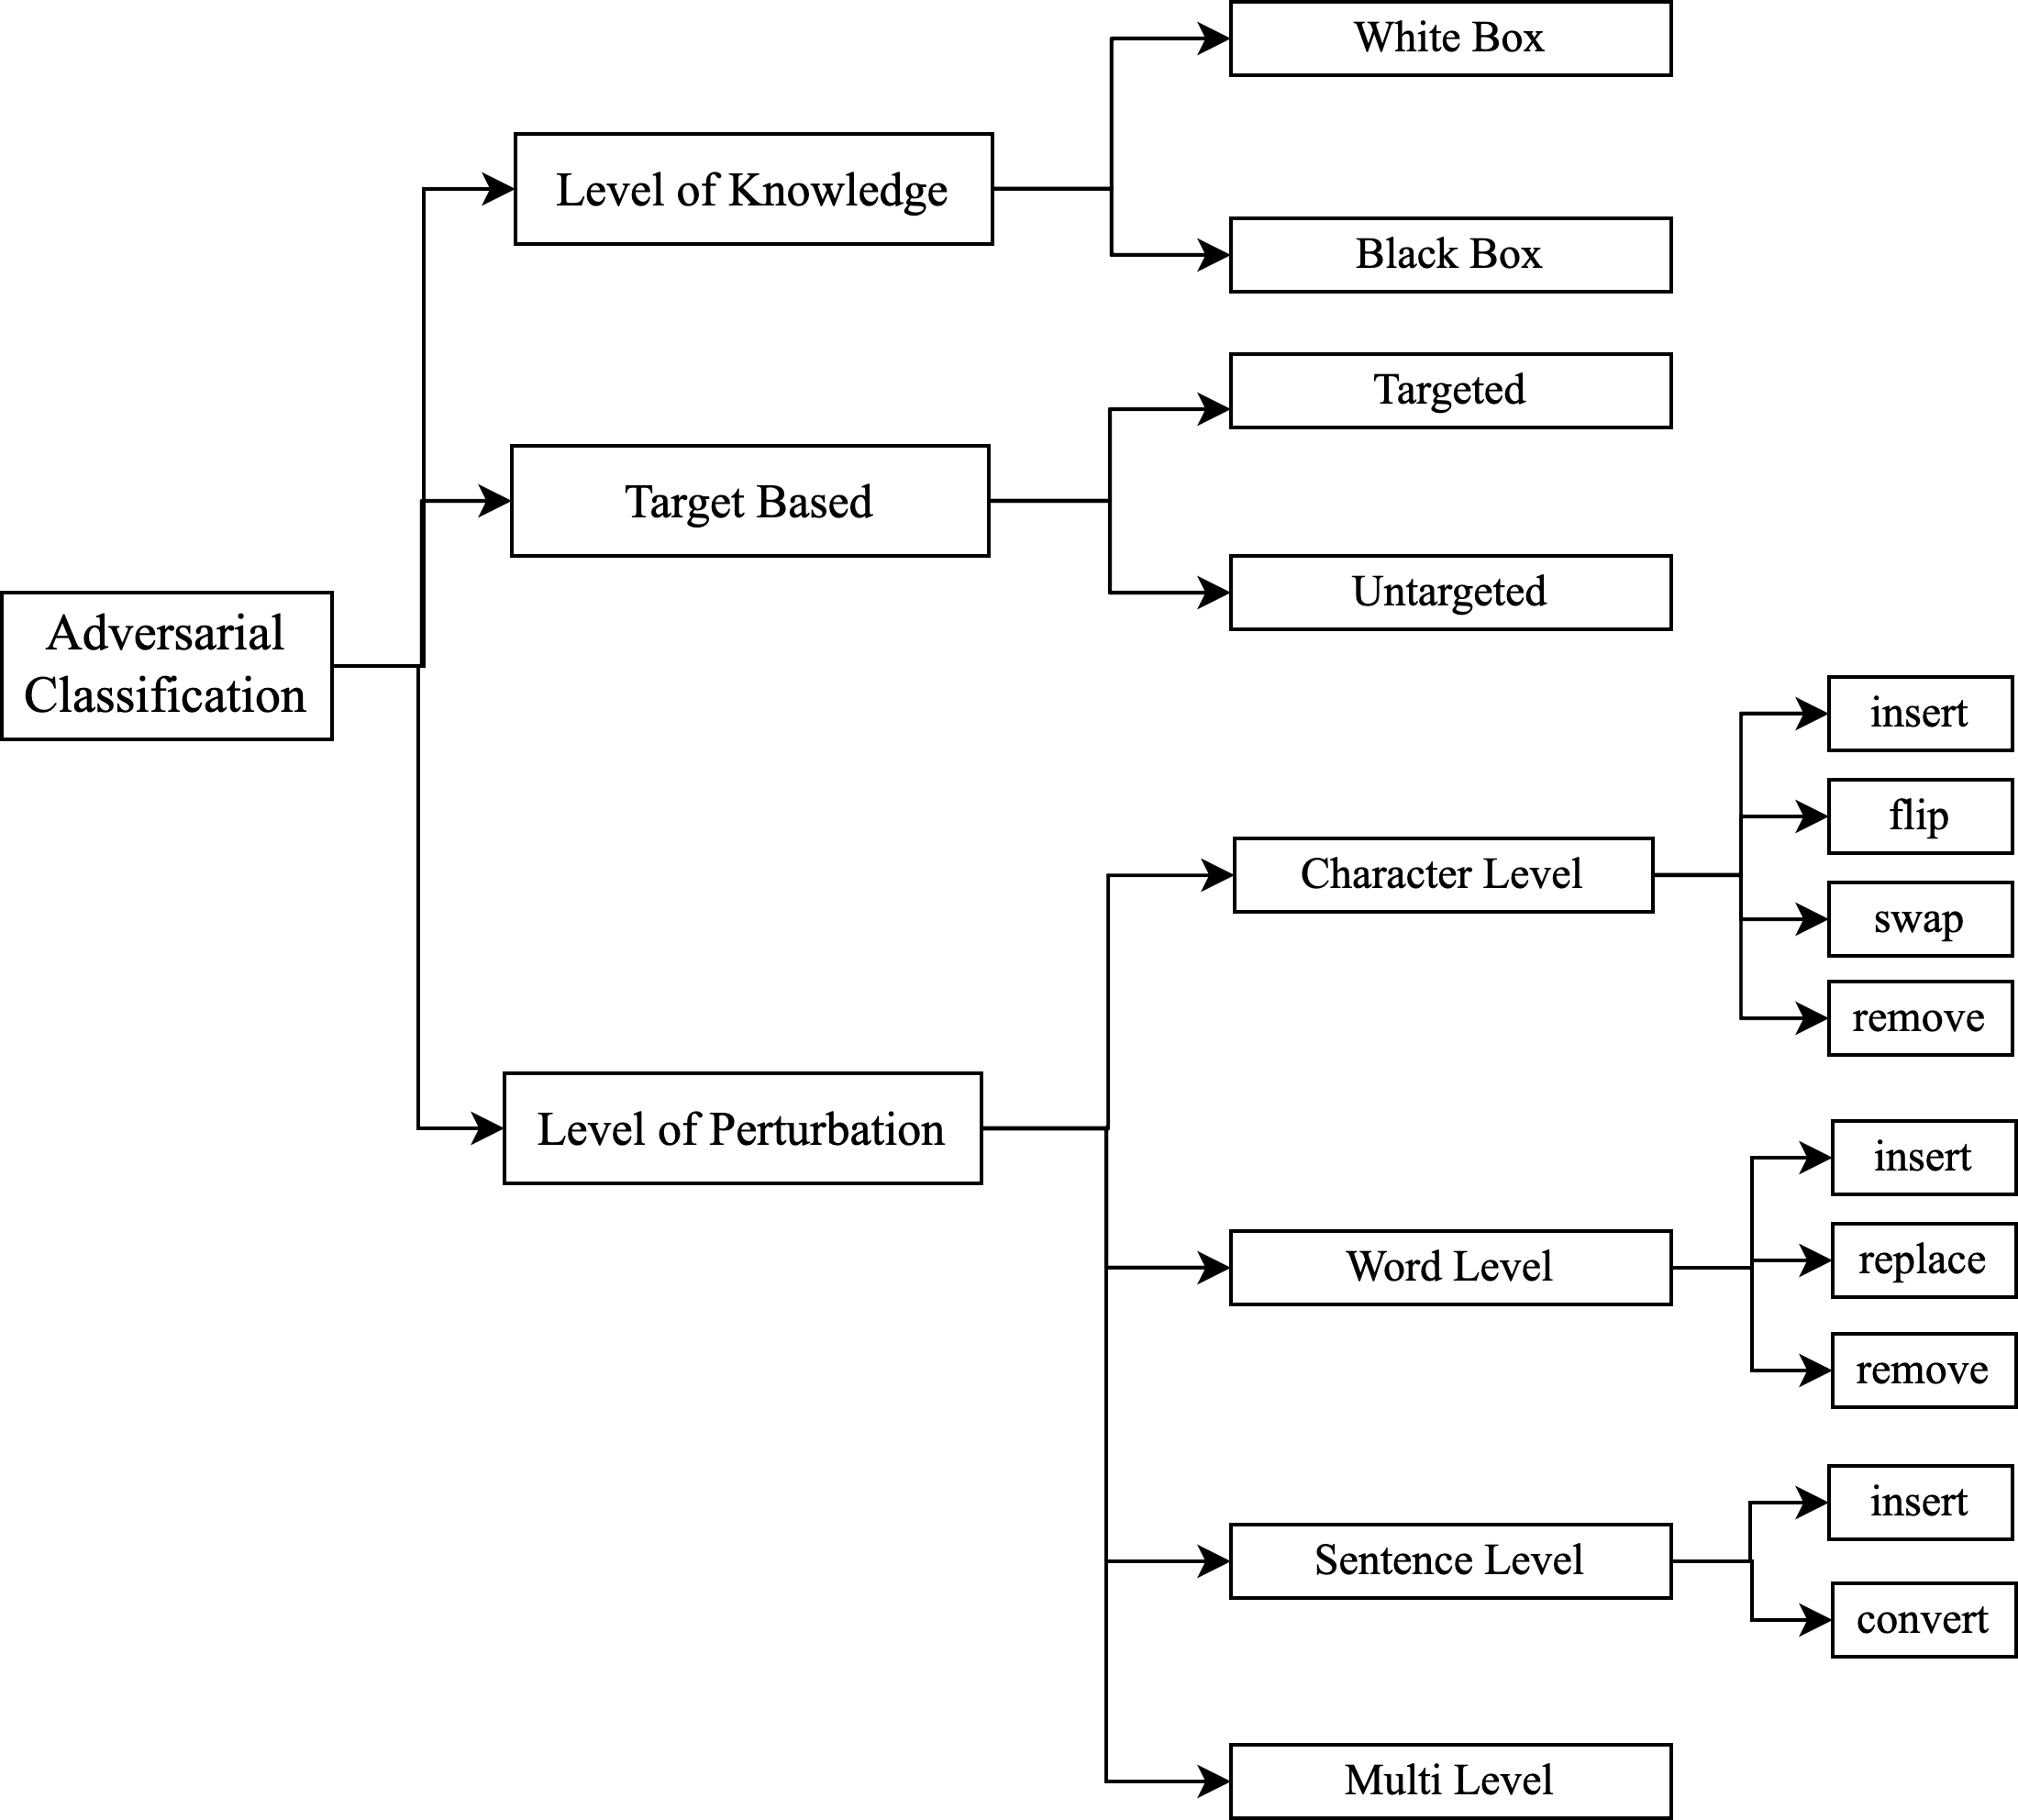
\includegraphics[width=0.65\linewidth]{img/attack_classification.png}
    \caption[Adversarial attacks classification diagram]{Different adversarial attack classification based on different aspect.}
    \label{fig:attack_classification}
\end{figure}
As mentioned in section \ref{subsection:definition}, when an attacker intentionally attempts to sabotage a model based on a specific class classification, it could be classified as targeted attack, whereas if the attacker just has the aim of sabotaging the model without depending on class classification, it would be untargeted attack.\\
A word level of perturbation may result in an attacker inserting, replacing, and removing words. TextDeceptor \cite{saxena_textdecepter_2020} proposed text attack approach, where they rank sentences and words, and then replace them with similar words based on a cosine measure of similarity between word vectors, as well as considering the POS (part-of-speech) helps to determine the correct grammar. Furthermore, Yuan et al. \cite{zang_word-level_2019} proposed a Word-Level Textual Adversarial attack that uses sememe-based word substitution. Using sememe-based word substitution is supposed to be more accurate since the substituted word has probably retained its meaning. In accordance with their claim, their attacks have a 98.70\% success rate on the IMDB dataset.\\
A char-level attack involves inserting, flipping, removing, and swapping operations to create adversarial text attacks. In the proposed approach by Eger et al. \cite{eger_text_2019}, a visual perturber called VIPER replaces input characters with their visual nearest neighbours in visual embedding space.
In the sentence level, attackers try to convert the input sentence using back translation or parapharsing technique and/or  insert some sentences into the text. Yankun et al. \cite{ren_generating_2020}  developed an approach that generates real-world meaningful text automatically using a variational encoder and decoder model. However, the sentences are often different from the originals.

\subsection{Adversarial Training}
\label{subsection: adversarialtraining}
The goal of adversarial defenses is to achieve high test accuracy on both clean and adversarial examples \cite{zhou_defense_2020}. Two strategies are mainly discussed in the text domain to fight adversarial attacks, the first being proactively detecting adversarial text, and the second being model enhancement by using adversarial training.\\
 Detecting adversarial text mainly revolves around detecting unknown words and misspellings, which impose limitations on using only the original corpus vocabulary \cite{wang_towards_2021}. 
According to Goodfellow et al. \cite{goodfellow_explaining_2015}, including high quality adversarial examples in images can improve the robustness and generalization of machine learning models. Similarly in text domain, Belinkov et al.  \cite{belinkov_synthetic_2018} demonstrated in their experiments that mixed noise in text training samples can improve model robustness. In another experiment performed by Li et al. \cite{li_textbugger_2019}, showed that including TextBugger attack adversarial samples in training can also improve model performance and robustness against adversarial examples.\\
A fast gradient method (FSM) approach to text domain training was introduced by Miyato et al. \cite{miyato_adversarial_2017}, whereby methods generate adversarial examples by adding gradient-based perturbations to input samples with different normalization strategies.
However, research related to adversarial training of language models is few. Liu et al. \cite{liu_adversarial_2020} proposed adversarial training of BERT model using virtual adversarial training (VAT) technique \cite{miyato_virtual_2018}  during pre-training. However, their approach is computationally expensive and also based on gradient.\\
Furthermore, the mean teacher approach has shown comparative performance in the computer visualization domain and the model claimed to be comparatively robust \cite{tarvainen_mean_2018}. And, the performance of this approach in the text-domain, which incorporates language models with adversarial training tactics  and evaluation of approach against adversarial attack had open scope of work. In addition, proposed approach utilizes the language model capabilities of such as context rewriting and back translation as data augmentation techniques to create prominent adversarial unlabeled data. \\
Similar approaches have been utilized previously to generate adversarial sample. Siddhant et al.  \cite{garg_bae_2020}  proposed approach used BERT's masked language model (MLM) to generate possible adversarial examples. Therefore, one of the major motivations for this experiment is to generate prominent adversarial examples and develop strategies for incorporating them into training.

\chapter{Related Work}
\label{chapter:relatedwork}
In the area of adversarial training and defense mechanisms against attack, various types of techniques are studied and proposed. Still, the research in text-domain comparatively less than that in the image-domain \cite{wang_towards_2021}. And, very few researches deal in evaluating language models against adversarial attacks recipes and proposing a semi-supervised fine-tuning approach as well. In this section, work related to adversarial training on the text-domain, using language models and focusing on evaluating against adversarial attacks are discussed.  The search for related work is performed on scholarly website such as google scholar and arxiv. Furthermore, search texts were consist of semi-supervised, adversarial training, robustness and language models. Moving forward,  after getting the relevant paper further papers were found based on connected paper service \cite{noauthor_connected_nodate-1}.
Adversarial training are primarily based on two approaches: 1) Gradient-based 2) Data-augmentation based. \\
The objective in gradient-based  is to optimize the adversarial loss for the model by applying perturbations in the embedding space \cite{liu_adversarial_2020,goodfellow_explaining_2015,zhu_at-bert_2021,miyato_adversarial_2017,jiang_smart_2020-1}.  However, these studies are focused on increasing generalization instead evaluating against attack.\\
 Liu et al.\cite{liu_adversarial_2020} proposed a novel adversarial pre-training approach intended to increase the robustness and generalization of large neural language models called ALUM (Adversarial Training for Large Neural Language Models). Both pre-training and fine-tuning can be accomplished using the same approach. Due to inner maximization and complexity, adversarial training is often quite costly, and verification of proposed approaches under a variety of attacks still needs to be studied.\\
More recent approach is proposed by Danqinq et al.\cite{zhu_at-bert_2021}, in which adversarial training is done by fast gradient methods (FGM) \cite{miyato_adversarial_2017} and ensemble methods, in which multi-BERT model prediction assists in robustness. A proposed approach combines multiple BERT (BERT, SciB ERT, RoBERTa, ALBERT, and ELECTRA) and makes an average ensemble for all models to achieve superior performance. Large language models and internal maximization raise concerns about computational cost. Moreover, as mentioned previously, this approach is also completely focused on increasing generalization and performance under attack has not been evaluated.\\
As part of a noise-based approach, Si et al.\cite{si_better_2021}  proposed robust fine-tuning of language models by augmenting the training dataset and performing mix-up augmentation during training, hence the term AMDA (Adversarial and Mixup Data Augmentation). A mix-up augmentation is a linear interpolation of representations and labels pairs of training samples to create different virtual training samples. As per their experiments, the original accuracy for the BERT model is 91.27\% and the accuracy under attack is 14.83\%; however, BERT with AMDA had 91.10\% original accuracy and 31.52\% accuracy under attack. Model performance under attack has improved significantly with this approach, but original accuracy decreased.\\
One approach proposed by Bao et al.\cite{bao_defending_2021} which involves training a language model to classify the input text and also discriminate adversarial samples simultaneously. Their proposed approach also generates adversarial samples using TextFooler \cite{jin_is_2020}, applies frequency aware randomization to the adversarial training set, and finally combines it with the original training set. In IMDB data, this approach has shown marginal improvements in original accuracy from 92.4\% to 92.8\% of BERT model, but improvement in accuracy under attack, from 12.4\% to 89.2\%. However, further metrics related to adversarial attacks such as number of queries and word perturbation are not mentioned in their report.\\
Wang et al.\cite{wang_adversarial_2021-1} proposed gradient based synonym substitution method to quickly generate adversarial samples called Fast Gradient Projection Method (FGPM). The adversarial samples are claimed to very effective in attacking the models. Including this technique in training have shown significant improvement in robustness of models and they call this technique as Adversarial Training with FGPM enhanced by Logit pairing (ATFL). But, the proposed approach is verified against CNN, LSTM, Bi-LSTM model and only accuracy under attack is the only metric in the study to determine the robustness of the model.\\
In another study of Wang et al.\cite{wang_natural_2020-1}, a Synonym Encoding Method (SEM) is proposed as defense approach against adversarial attacks. According to this method,  encoding the clusters of synonyms to a unique encoding before input layer of a model can be effective against synonym based adversarial attacks in context of text classification. As per the experiment, BERT model has shown 0.2\% drop in accuracy for IMDB dataset and synonym based PWWS attack recipes. However, the proposed method efficient against synonym based attacks and only accuracy is considered as a sign of robustness in the model.\\
A different approach is proposed by Guo et al. \cite{guo_rosearch_2021} a search based approach called RoSearch, where the robust distilled version of language model are looked in search space of various student model. And, claimed that the proposed approach can improve the robustness from 7\% $\sim$ 18\% up to 45.8\% $\sim$ 47.8\%. This approach is focused to enhance the knowledge distillation of language models and only accuracy as a metric of evaluation.\\
As most relevant studies is discussed in the section, however, their are further studies which deal in robustness of the models \cite{wang_infobert_2020, shi_robustness_2020,jones_robust_2020,jiang_smart_2020,malkiel_mml_2019,liu_transfer_2019}.
Currently, adversarial samples are majorly generated using gradient methods and including them in training can increase accuracy of the models but studies related to verification of language model against attacks still an open scope of work. In addition, it is challenging to compare the performances of published approaches \cite{moradi_evaluating_2021} because of no standard evaluation framework. Hence, this master thesis is also trying to provide metrics specific to evaluation against adversarial samples.

%%%%%%%%%%%%%%%%%%%%%%%%%%%%%%%%%%%%%%%%%%%%%%%%%%%%%%%%%%%%%%%%%%%%%%%%%CHAPTER PROPOSED METHODOLOGY%%%%%%%%%%%%%%%%%%%%%%%%%%%%%%%%%%%%%%%%%%%%%%%%%%%%%%%%%%%%%%%%%%%%%%%%%%%%%%%%%%%%%

\chapter{ Methodology}
\label{chapter:methodology}
This chapter discusses about working of proposed approach, followed by attack recipes used to evaluate the model, and research question.

\section{Proposed Approach}
The proposed method calls for fine-tuning the BERT model using semi-supervised approach for classification tasks and utilizes the adversarial unlabeled dataset for the same. A pictorial representation of methodology is illustrated in the figure \ref{diag:advMTBERT}.\\
The proposed approach uses semi-supervised approach of fine-tuning language model and utilizes the prominent adversarial unlabeled data for training with labeled data. The approach first starts with creating adversarial samples for training. As shown in figure \ref{diag:advMTBERT}, after pre-processing the training dataset is being split into three equals parts and prominent adversarial unlabel data is created on three different data augmentation strategies i.e. 1) Synonym based, 2) Context based and, 3) Back translation based and further discussed in section \ref{section:dataaugmentation}.  Labels of those adversarial dataset is discarded hence called prominent unlabeled adversarial data. Then, these generated samples are combined together and shuffled. After creating prominent unlabeled adversarial data, semi-supervised training starts.\\
The proposed semi-supervised approach is based on the mean teacher approach implemented in computer visualization domain \cite{tarvainen_mean_2018}. In the mean teacher model, two identical models are trained with two different strategies called student and teacher model. In which, only student model is trained, however, during training exponential moving weights are assigned to the teacher. The intuition behind this approach can be understood as, instead taking average of many models decision, teacher model is a mean of consecutive students models weights hence mean teacher. \\
As shown in figure \ref{diag:advMTBERT}, two cost function plays important role while back-propagating i.e. classification cost and consistency cost. Classification cost ($C(\theta)$) is calculated as binary cross entropy between label predicted by student model and ground truth label $y$ given input $x$.  As in this master thesis, evaluation is performed against binary classification task, hence, binary cross entropy loss is used. However, loss function can be utilized as per task.\\
\begin{equation}
    \begin{aligned}
        C( \theta )=-y \log (f(x,\theta))-(1-y) \log(1-f(x,\theta))
        \label{eq:classification_cost}
    \end{aligned}
\end{equation}
 \begin{figure}[h!]
    \centering
    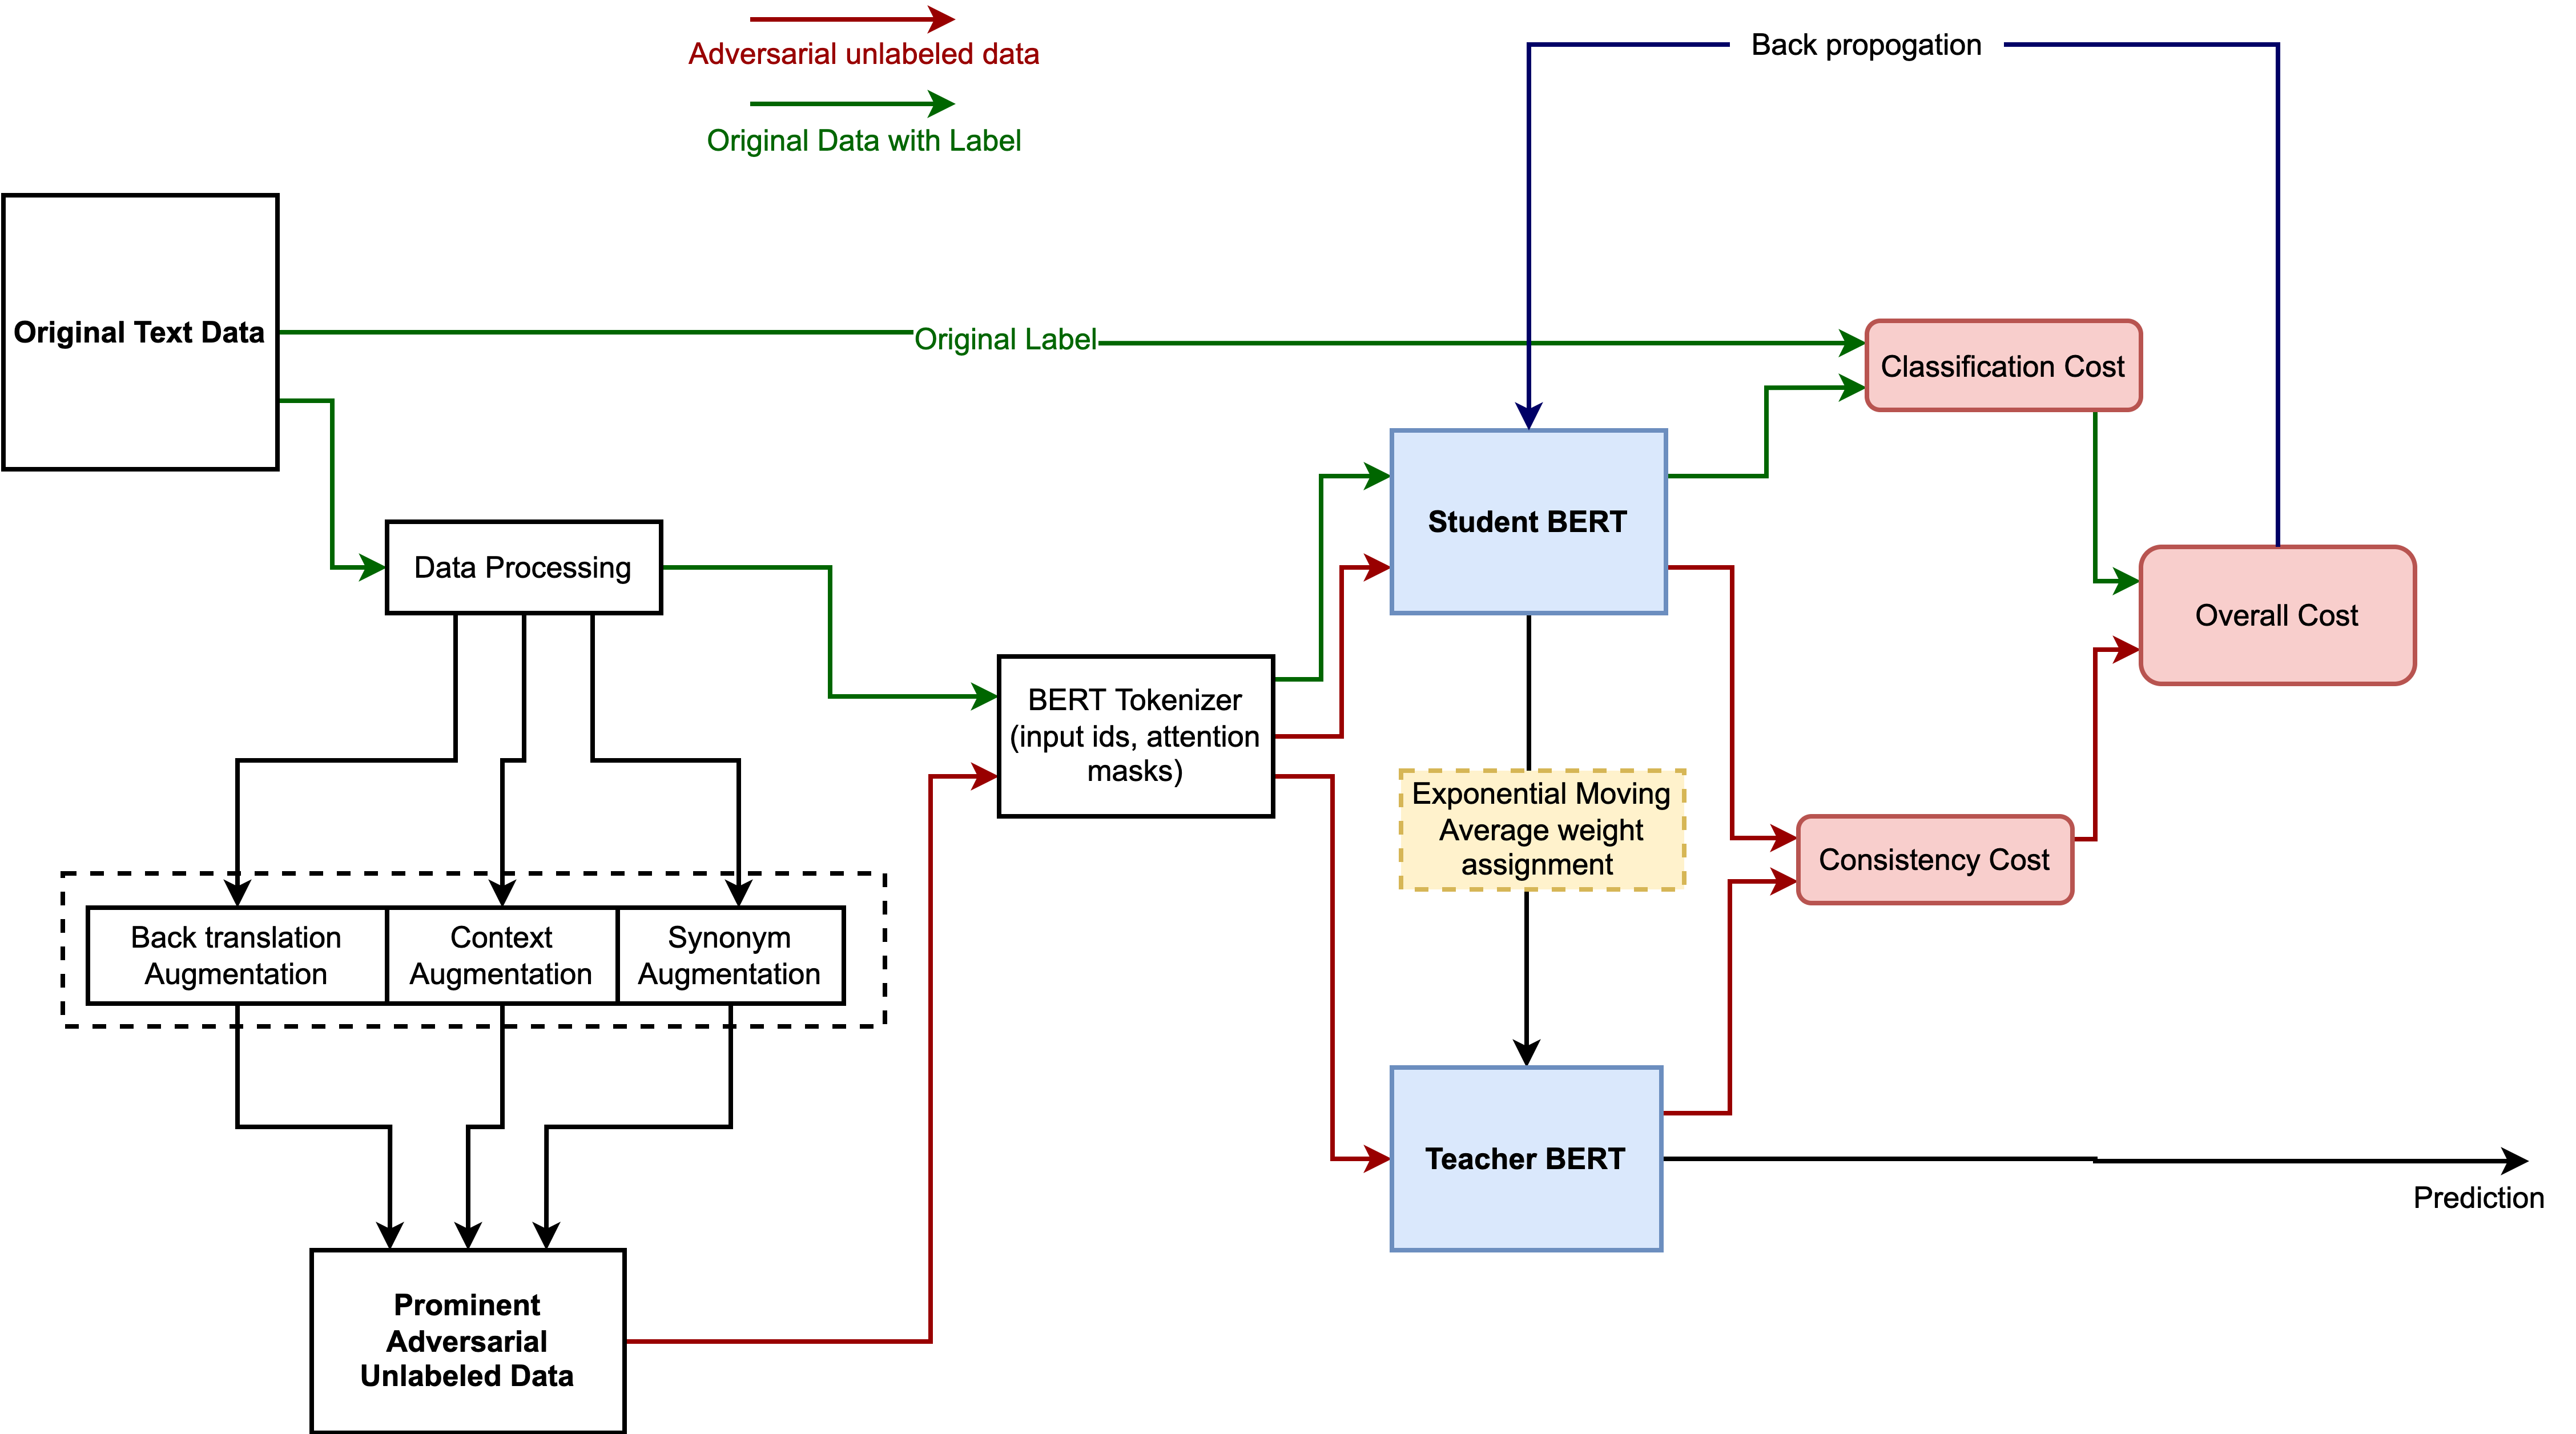
\includegraphics[width=1.1\textwidth]{img/Methodology.png}
    \caption[Training flow diagram of proposed approach]{Training flow diagram of proposed methodology }
    \label{diag:advMTBERT}
\end{figure}
The consistency cost ($J(\theta)$)  is the mean squared difference between the predicted outcomes of the student (weights $\theta$ and noise $\eta$) and teacher model (weights $\hat\theta$ and noise $\eta'$).  The mathematical declaration is as follows. 
\begin{equation}
    \begin{aligned}
        J( \theta )=\mathbb{E}_{x_{adv}}[\|f(x_{adv},\theta)-f(x_{adv},\hat\theta)\|^2]
        \label{eq:ADVconsistencycost}
    \end{aligned}
\end{equation}
While back propagating in student model, the overall cost ($\textit{O}(\theta)$) is calculated with given formula 
 \begin{equation}
     \begin{aligned}
         \textit{O}(\theta)= r C(\theta)+(1-r)J(\theta)
         \label{eq:overallcost}
         \end{aligned}
   \end{equation}
   When training, exponential moving average (EMA) weights of the student model are assigned to the teacher model at every step, and the proportion of weights assigned is controlled by parameter alpha ($\alpha$). As mentioned in equation \ref{eq:ema}, while assigning weights, teacher model holds its previous weights in alpha($\alpha$) proportion and ($1-\alpha$) portion of student weights. The proposed approach can be seen in form of algorithm \ref{alg:MeanTeacher}.
 \begin{equation}
     \begin{aligned}
         \hat\theta_t= \alpha\hat\theta_{t-1}+(1-\alpha)\theta_t
         \label{eq:ema}
         \end{aligned}
  \end{equation}

\begin{algorithm}[H]
    \caption{Mean Teacher Algorithm} \label{alg:MeanTeacher}
    \begin{algorithmic}
        \STATE \textbf{Data}: train set $\mathcal{(X,Y)}$,  Prominent Adversarial Unlabeled set($\mathcal{Z}$)
        \STATE \textbf{Hyper parameters}: \emph{r}, \emph{$\alpha$},\emph{epochs}
        \STATE \textbf{Create Model}: \emph{student($\theta$)}, \emph{teacher($\hat\theta$)} 
        \STATE  Train \emph{teacher} for n epoch
        \FOR{epochs = $1$ to $N$}
        \WHILE{$steps$}
        \STATE  \emph{student}($x$) = $y'$\
        \STATE Compute Classification cost ($C(\theta)$) = Binary Cross Entropy($y$,$y')$
        \STATE  \emph{student}($z$) = $y_s$
        \STATE  \emph{teacher}($z$) = $y_t$
        \STATE Compute Consistency cost $J(\theta)$=Mean Squared Error($y_s$,$y_{t}$)
        \STATE Compute Overall cost  $\textit{O}(\theta)= r C(\theta)+(1-r)J(\theta)$
        \STATE Compute \emph{gradients}, \textit{O}($\theta$) w.r.t  $\theta$ 
        \STATE Apply \emph{gradients} to $\theta$
        \STATE Update Exponential Moving average of $\theta$ to $\hat\theta$ i.e. $\hat\theta_t= \alpha\hat\theta_{t-1}+(1-\alpha)\theta_t$\
        \ENDWHILE
        \ENDFOR
    \end{algorithmic}
\end{algorithm}

\section{Text Attack Recipes and Tool}
\label{section:attackrecipes}
To evaluate the proposed approach, four black box attack recipes that satisfy lexical, grammatical, and semantic constraints have been selected. In order to evaluate baseline BERT model and proposed Mean Teacher BERT, we have used TextAttack python package\cite{morris_textattack_2020}  that provides attack recipes. Table \ref{table:attackRecipeExample} shows an example of perturbation. In this section, we will discuss their attacking principle, working, and characteristics.

\begin{table}[h!]
    \centering
    \hspace*{-1.2em}
    \resizebox{1.0\textwidth}{!}{
            \begin{tabular}{|p{3 cm}|p{9cm}|p{9cm}|}
                \hline
                Attack Recipe & Original Text & Perturbed Text \\
                \hline
                TextFooler & absolutely \textcolor{red}{fantastic} whatever i say wouldn t do this underrated movie the justice it deserves watch it now fantastic	 & absolutely  \textcolor{red}{sumptuous}  whatever i say wouldn t do this underrated movie the justice it deserves watch it now fantastic	 \\
                \hline
                TextBugger & absolutely \textcolor{red}{fantastic} whatever i say wouldn t do this underrated movie the justice it deserves watch it now fantastic	 & absolutely \textcolor{red}{fa?tastic} whatever i say wouldn t do this underrated movie the justice it deserves watch it now fantastic	 \\
                \hline
                PWWS & absolutely \textcolor{red}{fantastic} whatever i say wouldn t do this underrated movie the justice it deserves watch it now fantastic	 & absolutely \textcolor{red}{rattling} whatever i say wouldn t do this underrated movie the justice it deserves watch it now fantastic	 \\
                \hline
                BAE & absolutely \textcolor{red}{fantastic} \textcolor{red}{whatever} i say wouldn t do this underrated \textcolor{red}{movie} the justice it deserves \textcolor{red}{watch}  it now fantastic	 & absolutely \textcolor{red}{shit}   \textcolor{red}{something}  i say wouldn t do this underrated \textcolor{red}{film}   the justice it deserves  \textcolor{red}{of}  it now fantastic	 \\
                \hline
            \end{tabular}
              }
        \caption[ Perturbation examples of attack recipes.]{ Perturbation examples of attack recipes in this experiment.}
        \label{table:attackRecipeExample}
\end{table}

\subsection{TextFooler}
\label{subsection:textfooler}
Jin et al. proposed Textfooler \cite{jia_certified_2019}, a simple and effective adversarial attack generation strategy in black box settings which has characteristic of preserving the semantics, and grammar which they called utility-preserving adversarial examples as illustrated in figure \ref{diag:TextFoolerExp}. For better understanding the process is briefly explained in steps:
\begin{enumerate}
    \item  \textbf{Word Importance Ranking}: Given a sentence of words, they create a ranking of each word by calculating the change before and after deleting the words, called the importance score. NLTK and spaCy libraries are then used to remove stop words and preserve the grammar of the sentence. To improve the similarity of vectors, antonymy and synonymy are injected into vector space representations.
    The replacement policy completely depends on three factors: (1) Similar semantic similarity, (2) Fit in the surrounding context, (3) Attack on the model. Universal Sentence Encoder is used in the study proposed by Cer et al.\cite{cer_universal_2018} for encoding the sentence into a high-dimensional vector and calculating the cosine similarity between the sentences. Next, select replacement candidates with values above the preset threshold value and create a pool of candidates.
    \item \textbf{Replacement}: A candidate from a pool of candidates who can change the prediction of a target model is selected if there is an existing candidate with the highest cosine similarity between the original and adversarial sentences. If not, a lower confidence score for the label is chosen.
\end{enumerate}
Using IMDB movie review datasets, TextFooler has assessed the performance of BERT model under adversarial attack. In their experiment, the accuracy dropped significantly from 90.9\% to 13.6\% with perturbed words 6.1, number of queries to target model 1134, and average length of IMDB dataset 215. Additionally, TextFooler is computationally inexpensive and complexity increases linearly with text length. 
\begin{figure}[H]
    \centering
    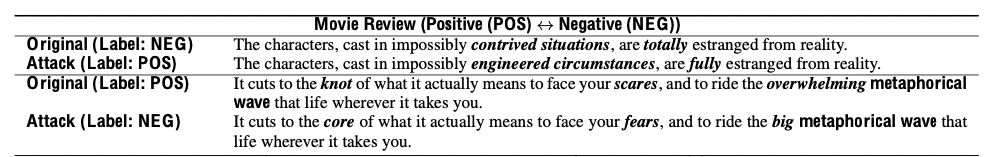
\includegraphics[width=1.0\textwidth]{img/textfooler_example.png}
    \caption[Example of TextFooler]{TextFooler example  \cite{jia_certified_2019} }
    \label{diag:TextFoolerExp}
\end{figure}

\subsection{TextBugger}
\label{subsection:textbugger}
The TextBugger system proposed by Jinfeng Li et al. \cite{li_textbugger_2019} uses misspelled words or characters that are visually and semantically similar to the original text. When tokens are misspelled, they become 'Unknown,' which is mapped to unknown token ids, causing machine learning models to behave incorrectly. On the other hand, studies show that similar misspellings can still be perceived by the reader \cite{rawlinson_significance_2007,alzantot_generating_2018}. Both character-level and word-level perturbation are targeted in this attack. Although Li et al.\cite{li_textbugger_2019}  proposed both white box and black box attack generation strategies, our report focuses on black box attacks. Here are three steps to black box attack generation:
\begin{enumerate}
    \item \textbf{Finding Important Sentences}: The importance score of individual sentences in an article is determined by confidence score of particular sentence by target model.
    \item \textbf{Finding Important Words}: The importance score of word is the difference between confidence of target model with word and without word.
    \item \textbf{Bugs Generation}: In TextBugger, they use five bugs generation strategy (1) \textbf{Insert}: Inserting space into words, (2) \textbf{Delete}: Deleting random character,
    (3) \textbf{Swap}: Swapping random adjacent character, (4) \textbf{Substitute-C}: Substitute character with visually similar characters, and (5)\textbf{ Substitute-W} : Replacing word with top-k nearest neighbour in context aware word vector space , as shown in figure \ref{diag:textbug}
\end{enumerate}

\begin{figure}[H]
    \centering
    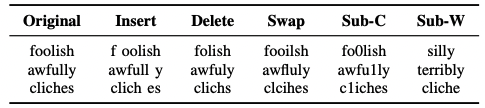
\includegraphics[width=.7\textwidth]{img/textbugger_5strat.png}
    \caption[Example of 5 bug generation strategies of TextBugger]{TextBugger 5 bug generation strategies \cite{li_textbugger_2019} }
    \label{diag:textbug}
\end{figure}

Using the IMDB movie review dataset, the TextBugger model is evaluated against LR, CNN, and LSTM and shows 95.2\%, 90.5\%, and 86.7\% accuracy with perturbed words of 4.9\%, 4.2\%, and 6.9\%. This report does not assess the effectiveness against BERT model. Comparatively to TextFooler, TextBugger generates adversarial attacks in much less time thanks to its sub-linear relationship to text length.

\subsection{Generating Natural Language Adversarial Examples through Probability Weighted Word Saliency (PWWS)}
\label{subsection:generatingadversarialexample}
Shhuhuai et al. \cite{ren_generating_2019} proposed a method for synonym and named entity (NE) replacement based on the words' saliency and classification probability, as well as a greedy algorithm called Probability Weighted Word Saliency (PWWS). When replacing a word with a synonym, there must be a significant change in classification probability as well as minimum saliency of the word. The approach can be summarized as follows:

\begin{enumerate}
    \item \textbf{Word Selection Strategy}:  
   Salience of a word is defined as its degree of change in classification probability if the word is set to unknown \cite{li_understanding_2017}. Calculating word saliency vectors for each word in a text, and then prioritizing the words based on degree of change in classification probability after replacement and minimum word saliency.
    \item \textbf{Replacement Strategy}: They searched WordNet for the synonyms of the words in order to find the replacement. Also, if the word is a Named Entity(NE), then replacing the NE with another NE of the same type appeared in the opposite class.
\end{enumerate}
Lastly, greedily replace words to make the model change the label. In addition to Word-based CNN \cite{kim_convolutional_2014},  LSTM \cite{hochreiter_long_1997},  and Char-based CNN \cite{zhang_character-level_2016}, this approach has been evaluated against other language models. According to the Bi-LSTM result, the accuracy dropped from 84.86\% to 2.00\% with perturbation 3.38\% for the IMDB dataset, example is shown in figure \ref{diag:pwwsexp}. However, the computational and time complexity of the proposed approach is higher than other methods.

\begin{figure}[h!]
    \centering
    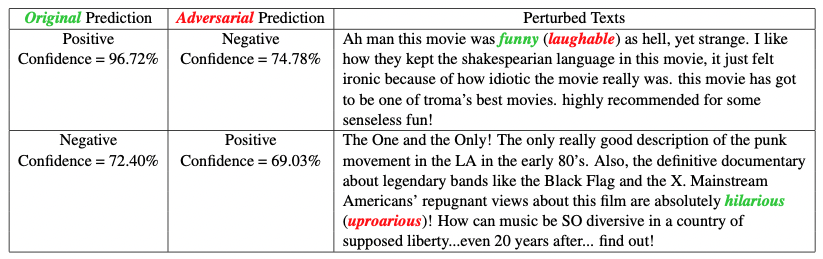
\includegraphics[width=.8\textwidth]{img/PWWSexample.png}
    \caption[Example of PWWS attack recipe]{Example attack of PWWS\cite{ren_generating_2019} }
    \label{diag:pwwsexp}
\end{figure}

\subsection{BAE: BERT-Based Adversarial Examples}
\label{subsection:bae}
The BERT masked language model (MLM) was employed by Garg et al. \cite{garg_bae_2020}  to generate adversarial examples. Based on their approach, they first calculate the importance of words by computing the decrease in probability of predicting the correct label after deleting that particular word, similar to Textfooler \cite{jia_certified_2019}  and PWWS \cite{ren_generating_2019}. Using the BERT MLM model, replace a specific word with a MASK token and let the model predict context-specific words. Using the Universal Sentence Encoder \cite{cer_universal_2018} and removing words that do not fall into a similar part-of-speech(POS) as the original word, filter the top K tokens using the most similarity score (Threshold 0.8). Substitute top K(50) tokens for the original word, iterate from most similar token in decreasing order until attack is successful and try all combinations. Figure \ref{diag:baeexp} shows a schematic working diagram.
\begin{figure}[H]
    \centering
    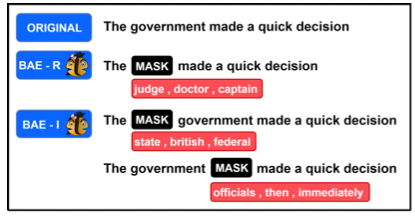
\includegraphics[width=.5\textwidth]{img/BAEexample.png}
    \caption[Schematic working and example of BAE attack recipe]{Schematic working and example of BAE\cite{garg_bae_2020} }
    \label{diag:baeexp}
\end{figure}

\section{Research Questions}
\label{section:researchquestions}
The objective of proposed approach is to study the effects on model performance by using comparatively simpler adversarial examples which involves utilizing capabilities of language models such as context rewriting, and back translation. \\
Hence, the major research question of this thesis is : \textit{Proposed approach of fine-tuning can enhance the performance of language models under attack without compromising on generalization.} \\
Moreover, it is  also hypothesized that robustness can be achieved by learning more representations and regularizing the model by not allowing model to learn the deep insight of the representation to prevent over-fitting as well. And, exponential moving averages (EMA) play an essential role in increasing generalization and performance under attack. \\
 Furthermore, two studies which can be verified against this master thesis i.e. 1) Averaging weights over time tends to produce a more accurate model than using the final weights directly \cite{polyak_acceleration_1992} and teacher model is an average of consecutive student models, therefore, teacher model should be more accurate. 2) Adding data augmentation can enhance model robustness \cite{belinkov_synthetic_2018}; hence, the proposed model approach should also perform well under attack.\\
This thesis attempts to answer the question by constructing a teacher model using proposed semi-supervised approaches and comparing the generalization of both conventional and proposed fine-tuning methods in terms of different evaluation metrics. \\
The robustness of this experiment will be evaluated using metrics such as original accuracy, accuracy under attack, average word perturbation, average number of queries, and attack success rate, which are discussed briefly in  section \ref{section:metrics}. Hence, the hypothesis would be that the proposed approach would have higher original accuracy, accuracy under attack, and require more queries and perturbations to get attacked. Additionally, the attack success rate is lower. The model performance is evaluated using four different attack recipes discussed in section \ref{section:attackrecipes}. \\
In addition, the experiment also attempts to understand the robustness of model by examining the confidence score distribution. A model that does not allow attack recipes to be misclassified with high confidence is a sign of robustness.
%%%%%%%%%%%%%%%%%%%%%%%%%%%%%%%%%%%%%%%%%%%%%%%%%%%%%%%%%%%%%%%%%%%%%%%%%CHAPTER DATASET%%%%%%%%%%%%%%%%%%%%%%%%%%%%%%%%%%%%%%%%%%%%%%%%%%%%%%%%%%%%%%%%%%%%%%%%%
%%%%%%%%%%%%%%%%%%%%%%%%%%%%%%%%%%%%%%%%%%%%%%%%%%%%%%%%%%%%%%CHAPTER EXPERIMENTS%%%%%%%%%%%%%%%%%%%%%%%%%%%%%%%%%%%%%%%%%%%%%%%%%%%%%%%%%%%%%%%%%%%%%%%%%%%%%%%%%

\chapter{Experiment Setup}
\label{chapter:experiment}

\section{Dataset}
\label{label:dataset}
To assess the performance of baseline and proposed model two dataset were selected i.e. 1) Covid-19  fake tweets dataset \cite{patwa_fighting_2021} provided at Codalab competition, and 2) IMDB review binary classification dataset were selected. \\
The IMDB dataset is a sentiment classification dataset\cite{maas_learning_2011-1} that contains movie reviews of the user and contains positive and negative ratings, and it is primarily used in classification and adversarial attack papers.Due to computational limitations, we have filtered and sampled only datasets whose length is between 6 and 150 as the augmentation process takes quite a while. This leaves us with 6000 samples to train and test our model. The train and test sizes are shown in table \ref{table:train/test table }. Additionally, we have sampled 6000 training labeled samples to create an augmented unlabeled dataset. Filtered datasets have an average text length of 127. The label distribution in training datasets is completely balanced.\\
Covid-19 fake tweets dataset is a recent dataset specifically for classifying fake tweets related to COVID-19 with label as fake or real. Covid-19 fake tweets dataset sized 8000 and we have fully utilized this dataset. Contrary to the IMDB dataset, the Covid-19  fake tweets dataset has an average length of 25, as shown in table \ref{table:Length stat }. Furthermore, as Covid-19  fake tweets dataset has mostly hashtags and comparatively less correct English words.\\
Therefore, the intention of observing the models behavior under recent dataset which has comparatively lesser text length and vocabulary size led to select this dataset.

\begin{table}[!h]
\centering
\begin{tabular}{ |c|c|c|c|c|c| }
\hline
Dataset & Train & Test  & Aug. Unlabeled \\
\hline
codalab (Positive/Negative) & 3199/2891 & 1071/969 & 6090 \\
\hline
IMDB (Fake/Real) & 3025/3025 & 1000/1000 & 6050  \\
\hline
\end{tabular}
\caption[Train/Augment test data]{Train/ Test split details of dataset }
\label{table:train/test table }
\end{table}

\section{Data Pre-processing and Exploration}
\label{section:datapreproc}
Since language models learn the context of sentences, they are least affected by stop words. Therefore, removing those words may affect the performance. Therefore, one of the benefits of the language model is its negligible requirement for data cleaning or no data cleaning at all. Here are the preprocessing steps we performed:
\begin{enumerate}
\item  HTML tags removal.
\item Digit removal.
\item Lower casing.
\item  Punctuation removal.
\end{enumerate}
This particular task was accomplished by using the texthero python library, which offers functions related to data pre-processing and exploration.

\subsubsection{Data Exploration}
\label{subsection:dataexploration}
The mentioned models were trained with almost equal distributions of labels in training and test data, and the same training data that was used to generate unlabeled augmented data via the proposed method is shown in \ref{table:train/test table }.
During experiments, various exploration technique were utilized such as word cloud, word distribution with/without respect to classes in dataset, and length distribution. Those information can be seen in provided github project. However, the most relative information about the dataset i.e. about length is provided in table \ref{table:Length stat } and figure \ref{fig:lendist}.
The Covid-19 Fake tweets dataset is shorter than the IMDB dataset. The purpose for using two distinct length datasets is to better understand the behavior of models and attack recipes in relation to the length.
\begin{table}[!h]
\centering
\begin{tabular}{ |c|c| }
\hline
Dataset &  Avg. Length  \\
\hline
codalab & 25  \\
IMDB & 127  \\
\hline
\end{tabular}
\caption[Length details of datasets]{Length details of both the datasets.}
\label{table:Length stat }
\end{table}
\begin{figure}[ht]
     \hspace*{3.0em}
    \begin{minipage}[b]{0.4\linewidth}
        \centering
        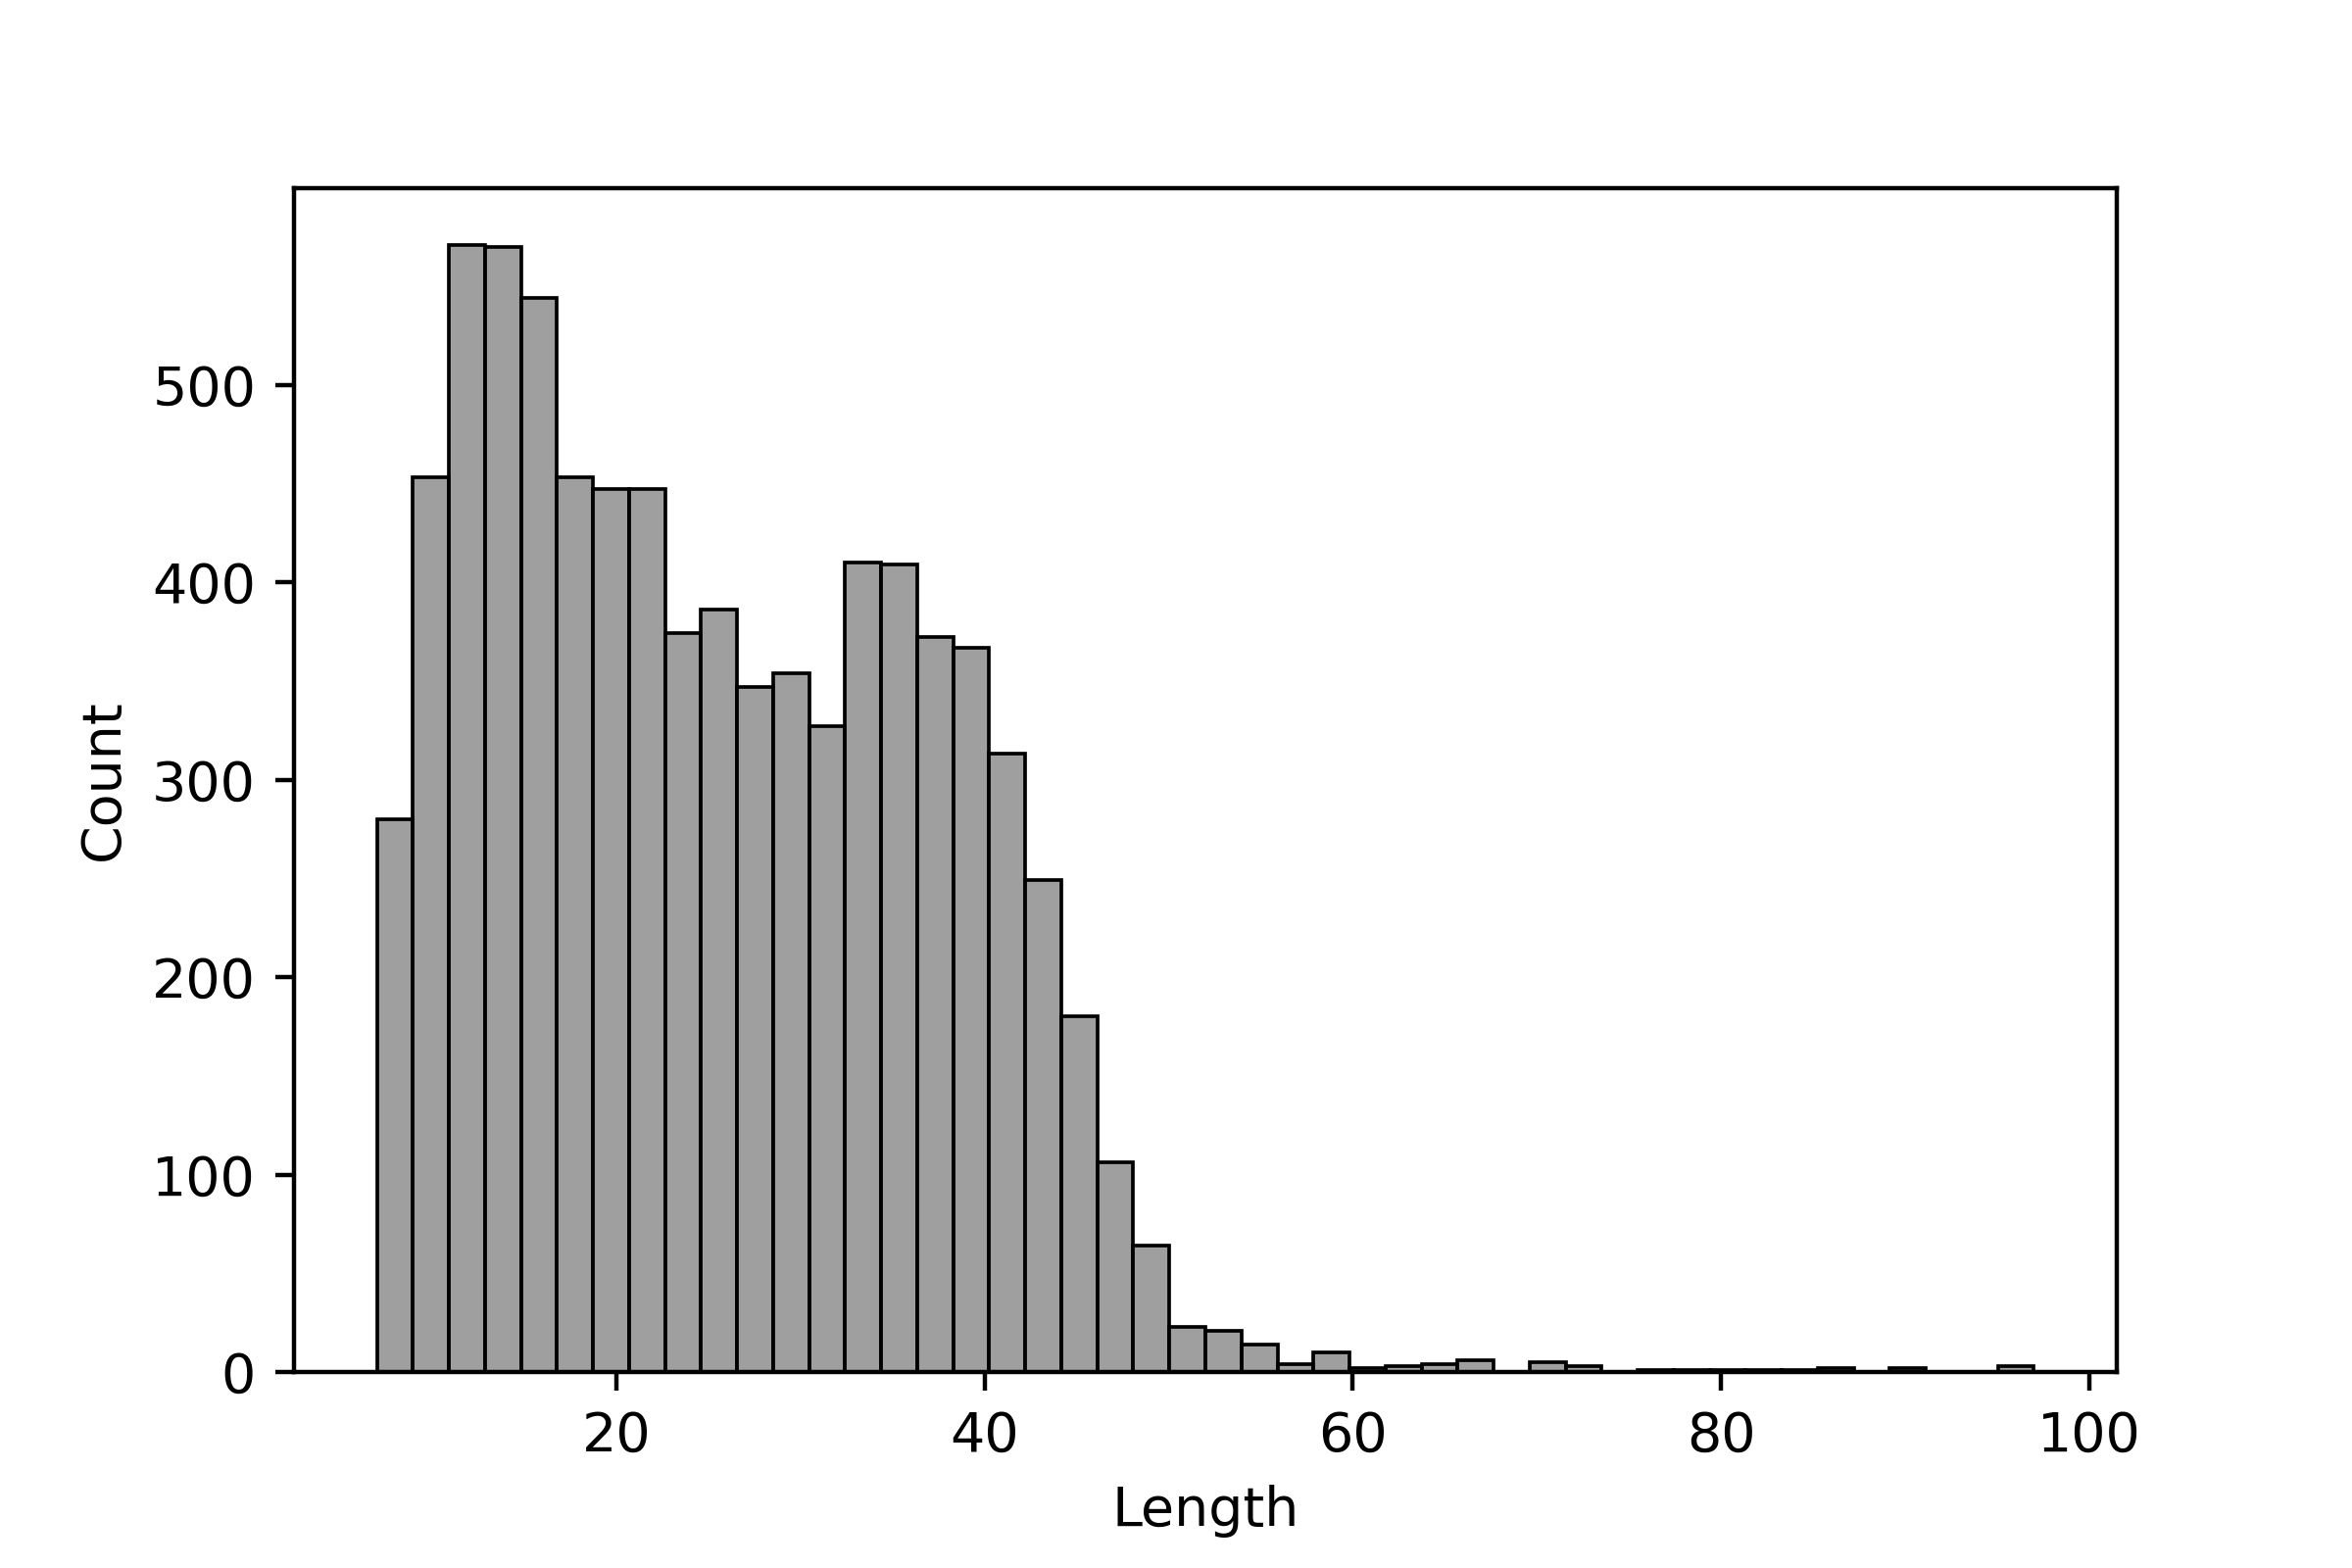
\includegraphics[width=\textwidth]{img/fakenewsLengthdist.png}
        \caption{Length distribution of Covid-19 fake tweets dataset.}
        \label{fig:fklendist}
    \end{minipage}
    \hspace{0.1cm}
    \begin{minipage}[b]{0.4\linewidth}
        \centering
        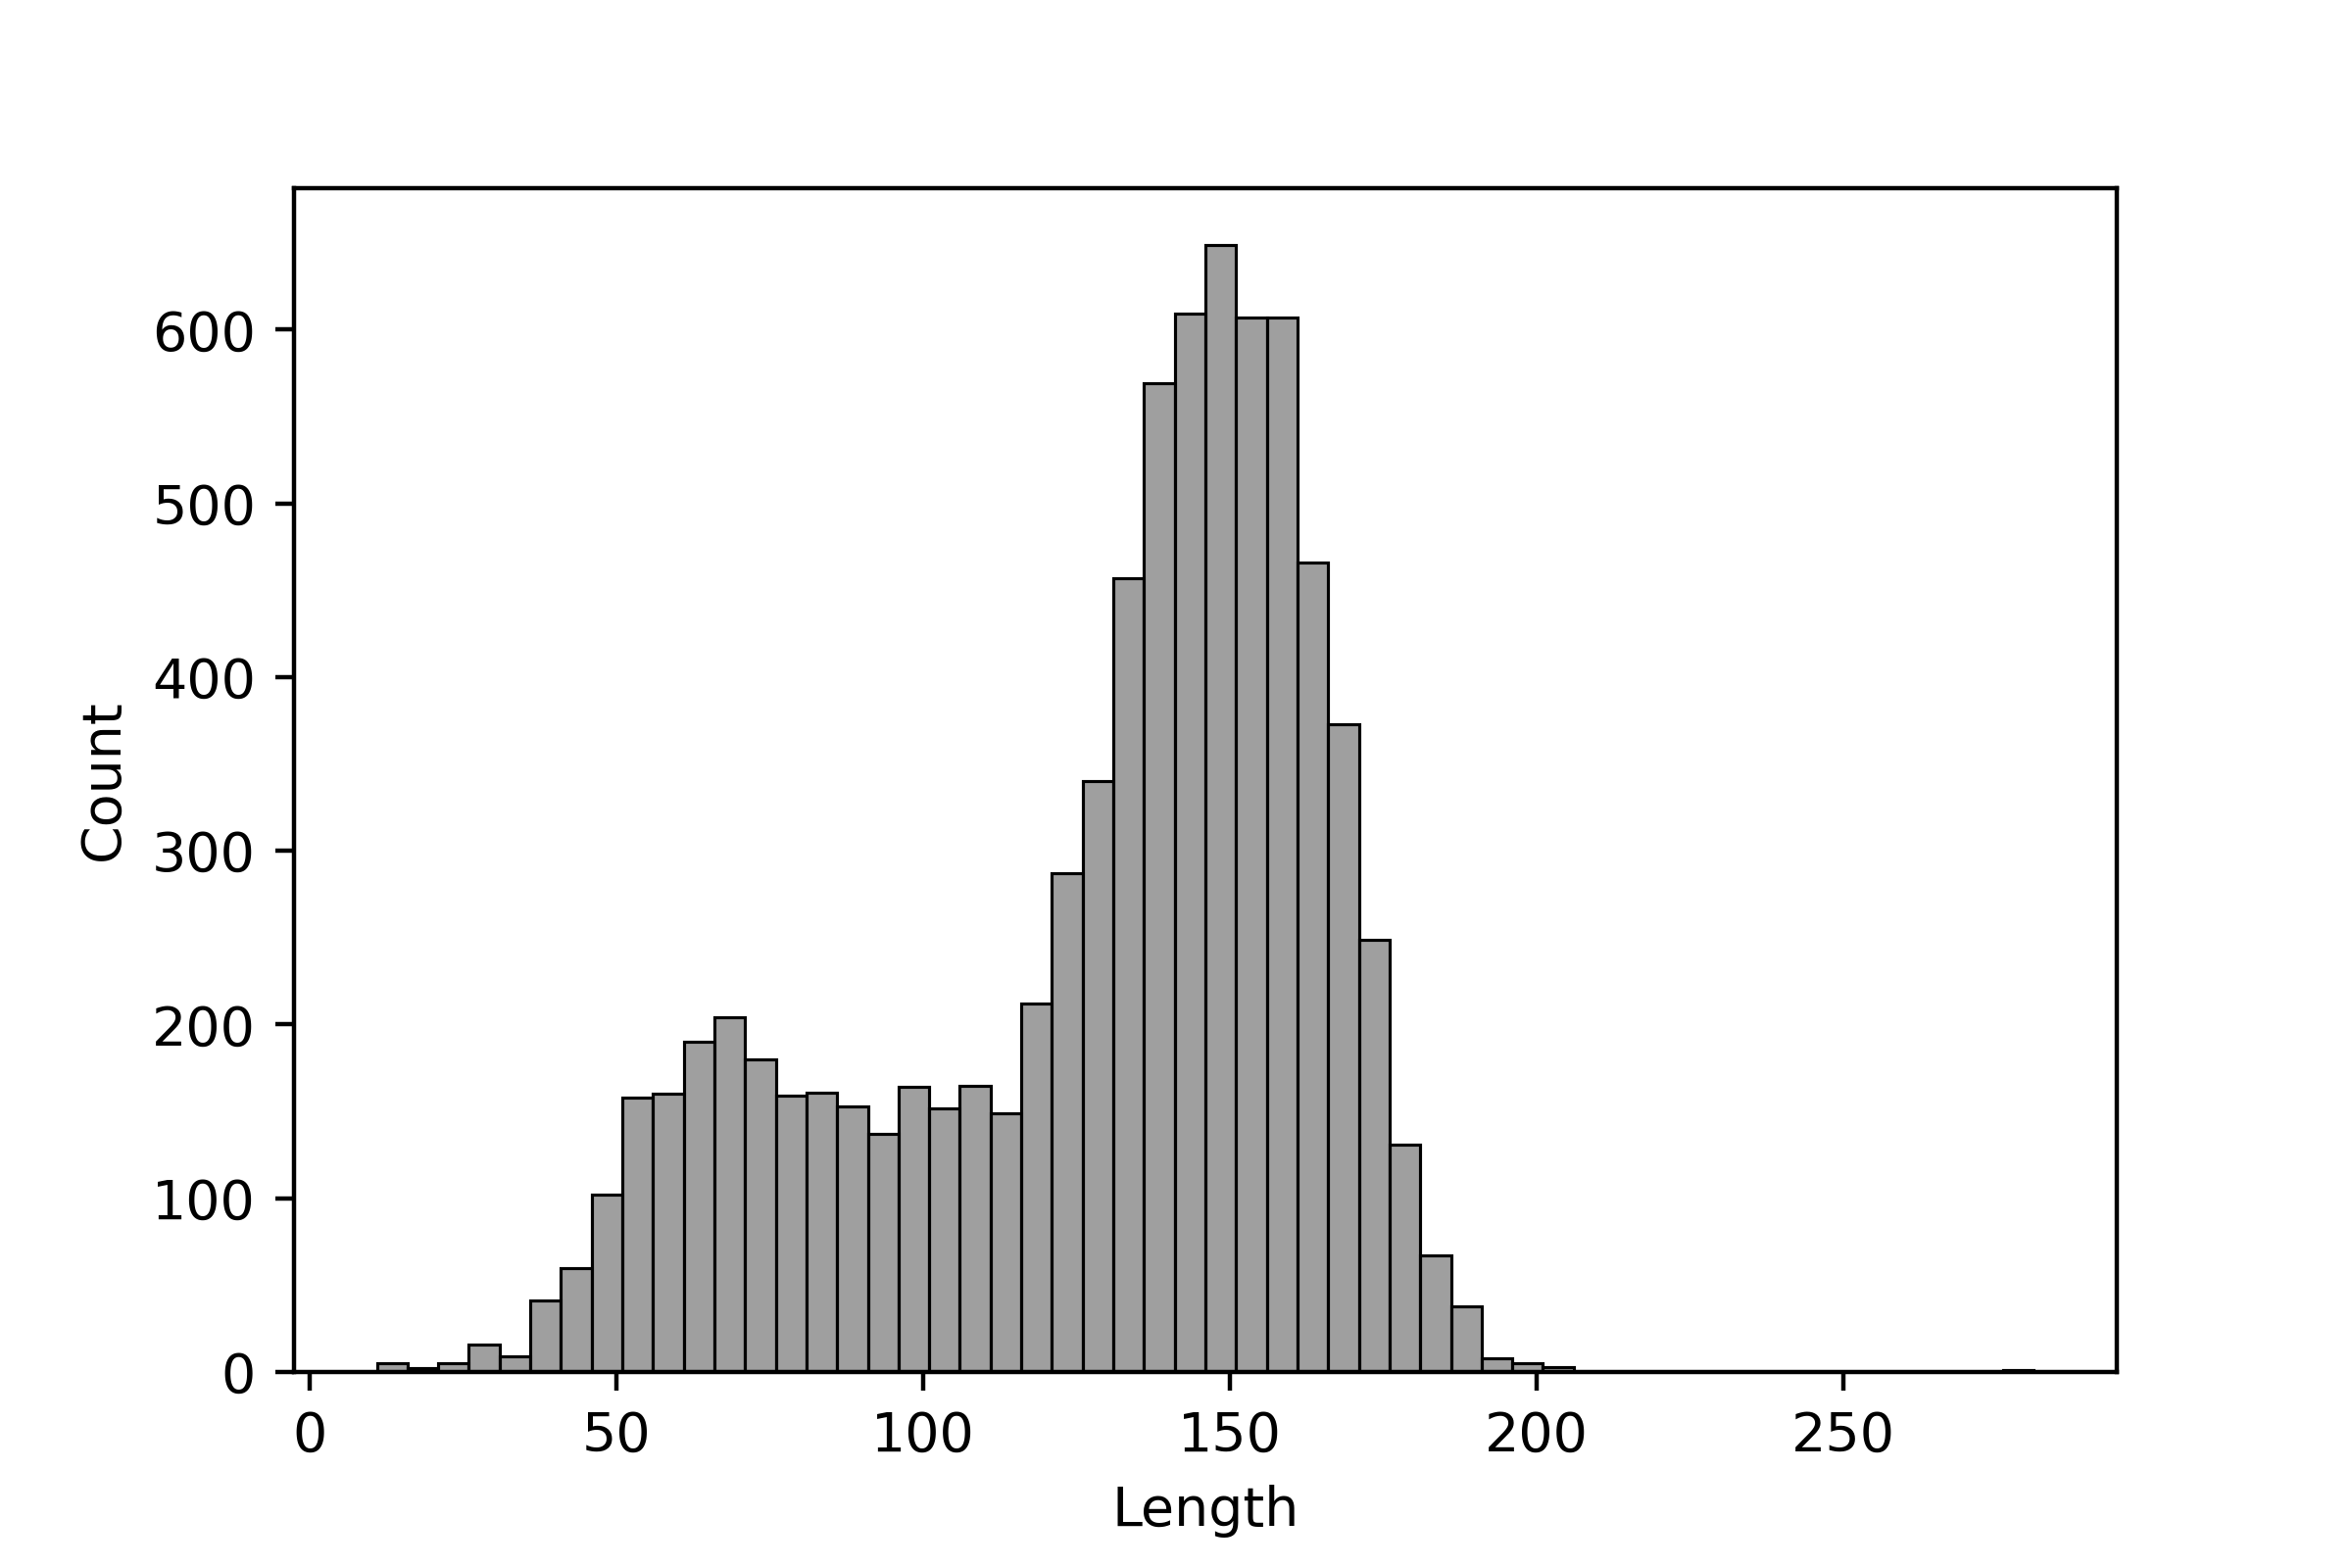
\includegraphics[width=\textwidth]{img/ImdbLengthdist.png}
        \caption{Length distribution of IMDB Dataset.}{}
        \label{fig:imdblendist}
    \end{minipage}
    \caption[Length distribution of Covid-19 fake tweets and IMDB Dataset]{\small Length Distribution of Covid-19 fake tweets and IMDB Dataset.}
    \label{fig:lendist}
\end{figure}

%\begin{figure}[H]
%    \centering
%%    \hspace*{1.0em}
%    \begin{subfigure}
%        \centering
%        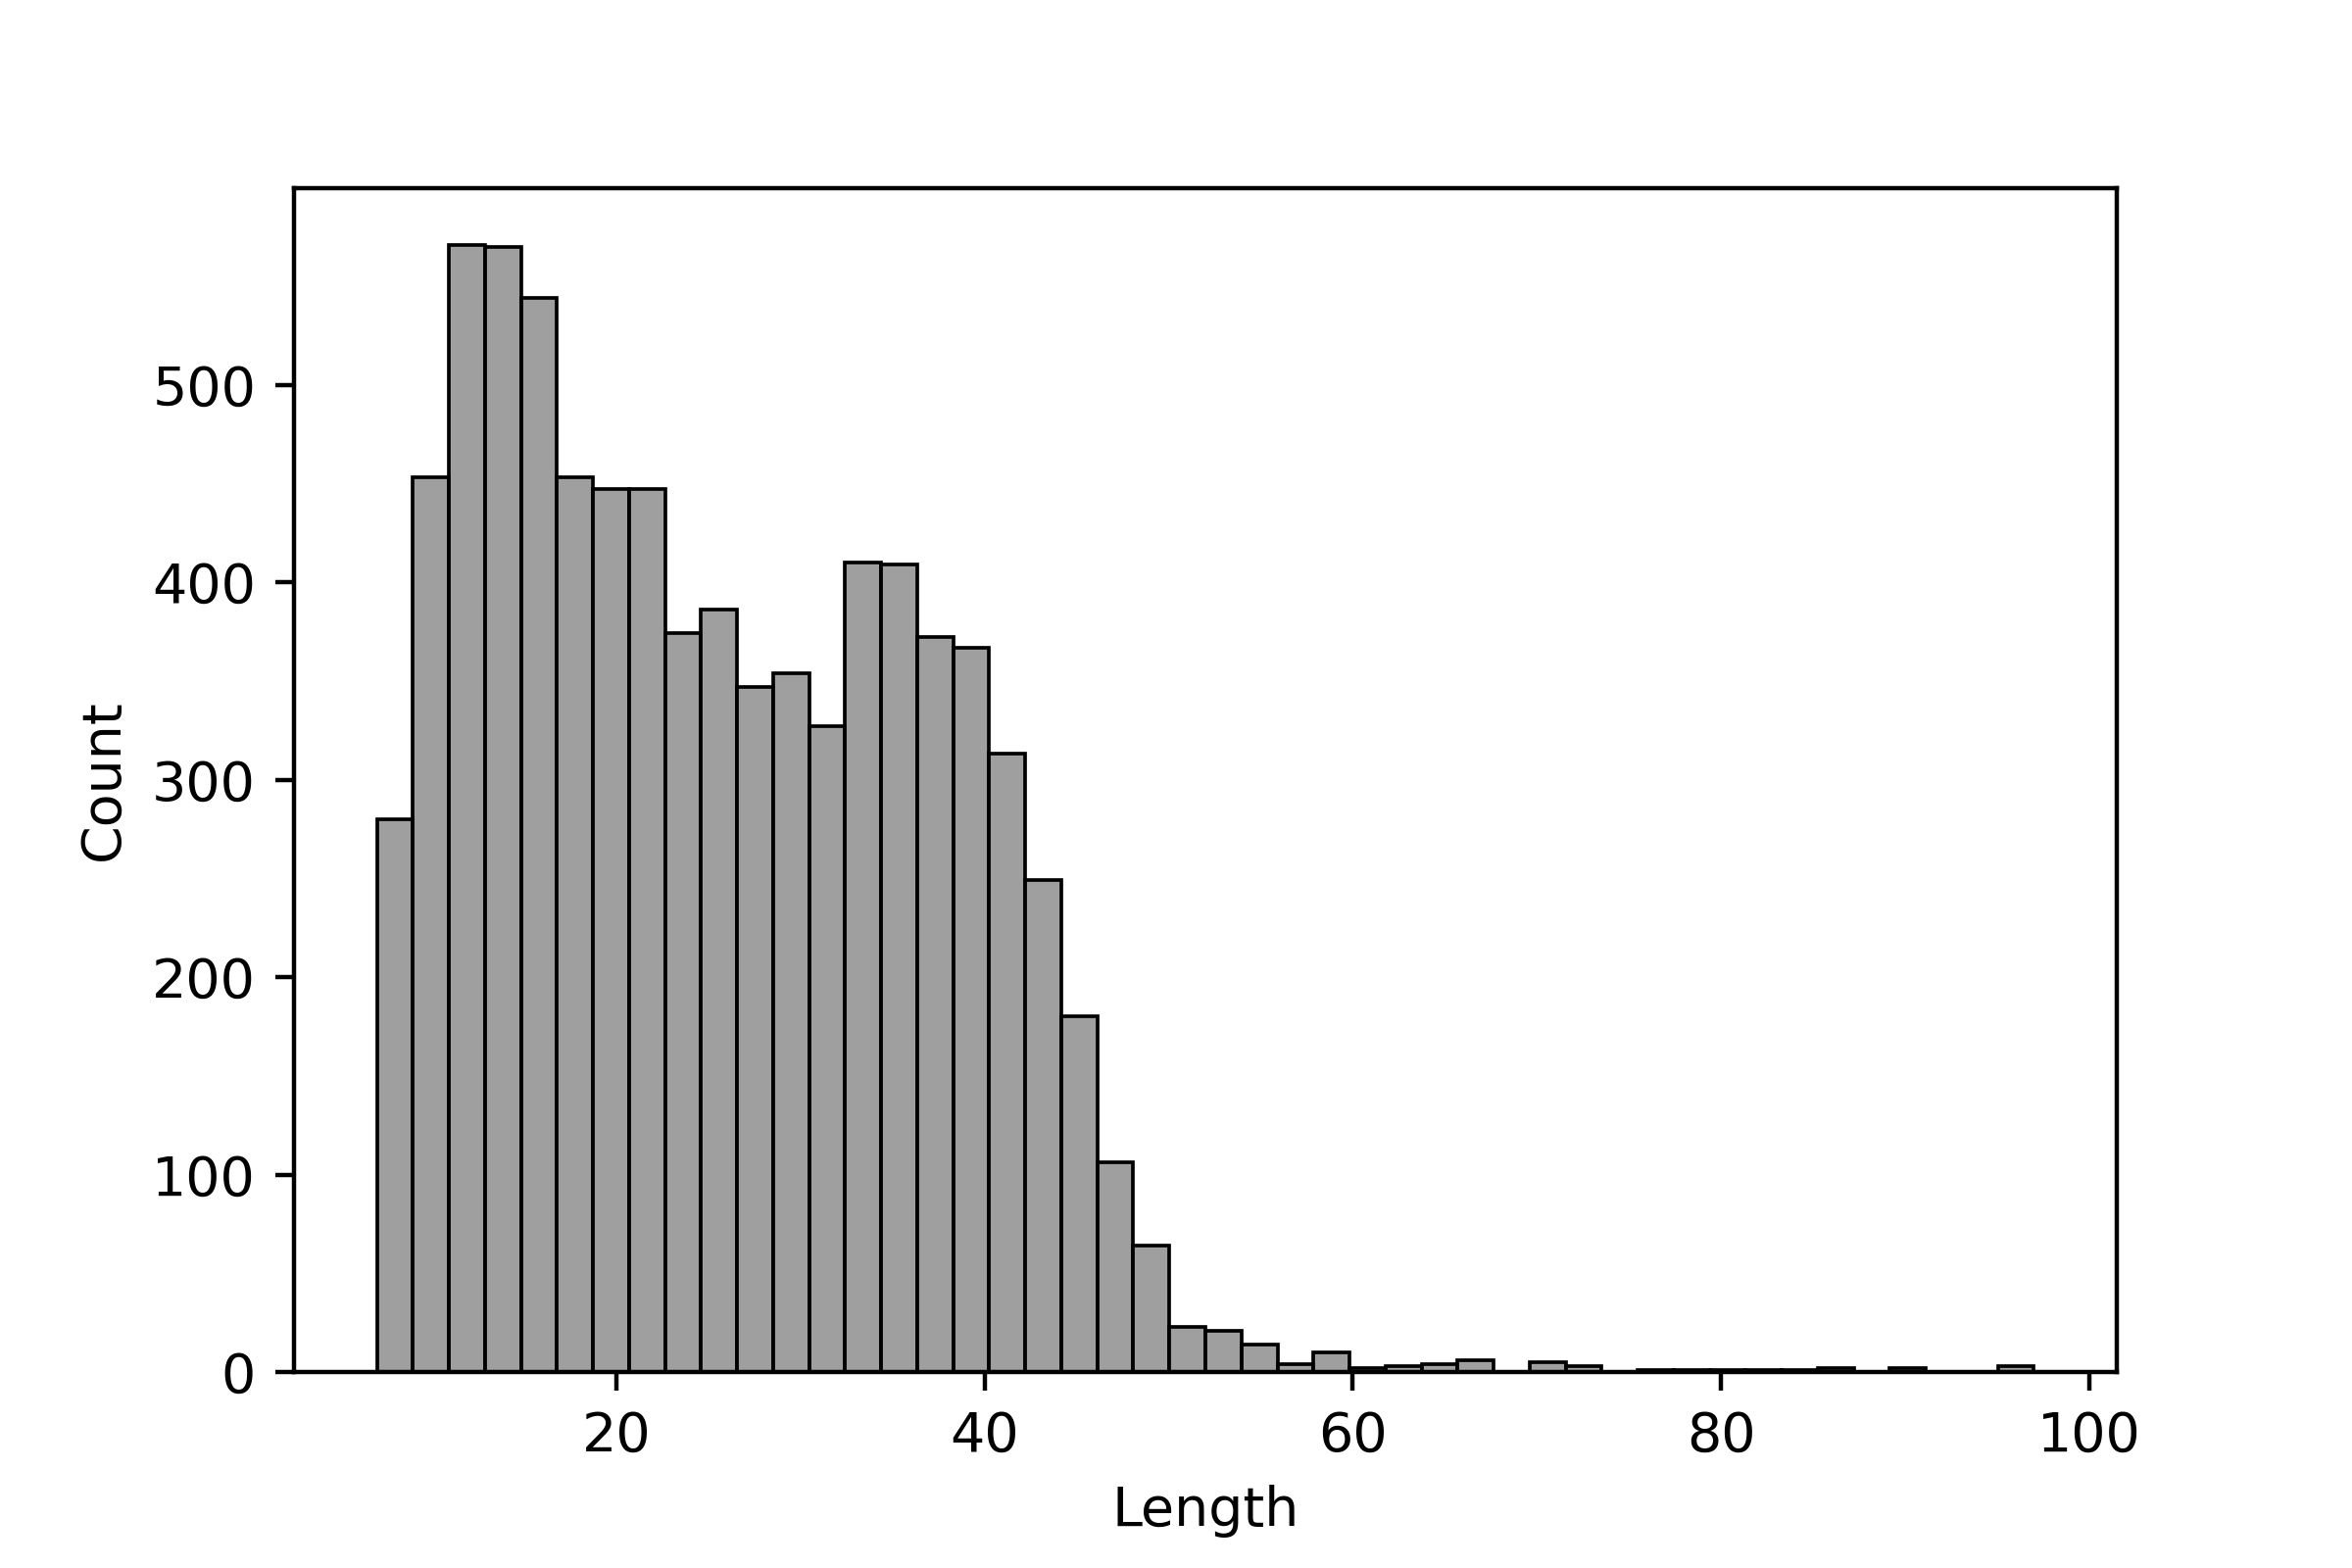
\includegraphics[width=.5\linewidth]{img/fakenewsLengthdist.png}
%        \caption{Covid-19 fake tweets dataset.}{}
%           \label{fig:}
%    \end{subfigure}
%%    \hspace*{1.8em}
%    \begin{subfigure}
%        \centering
%        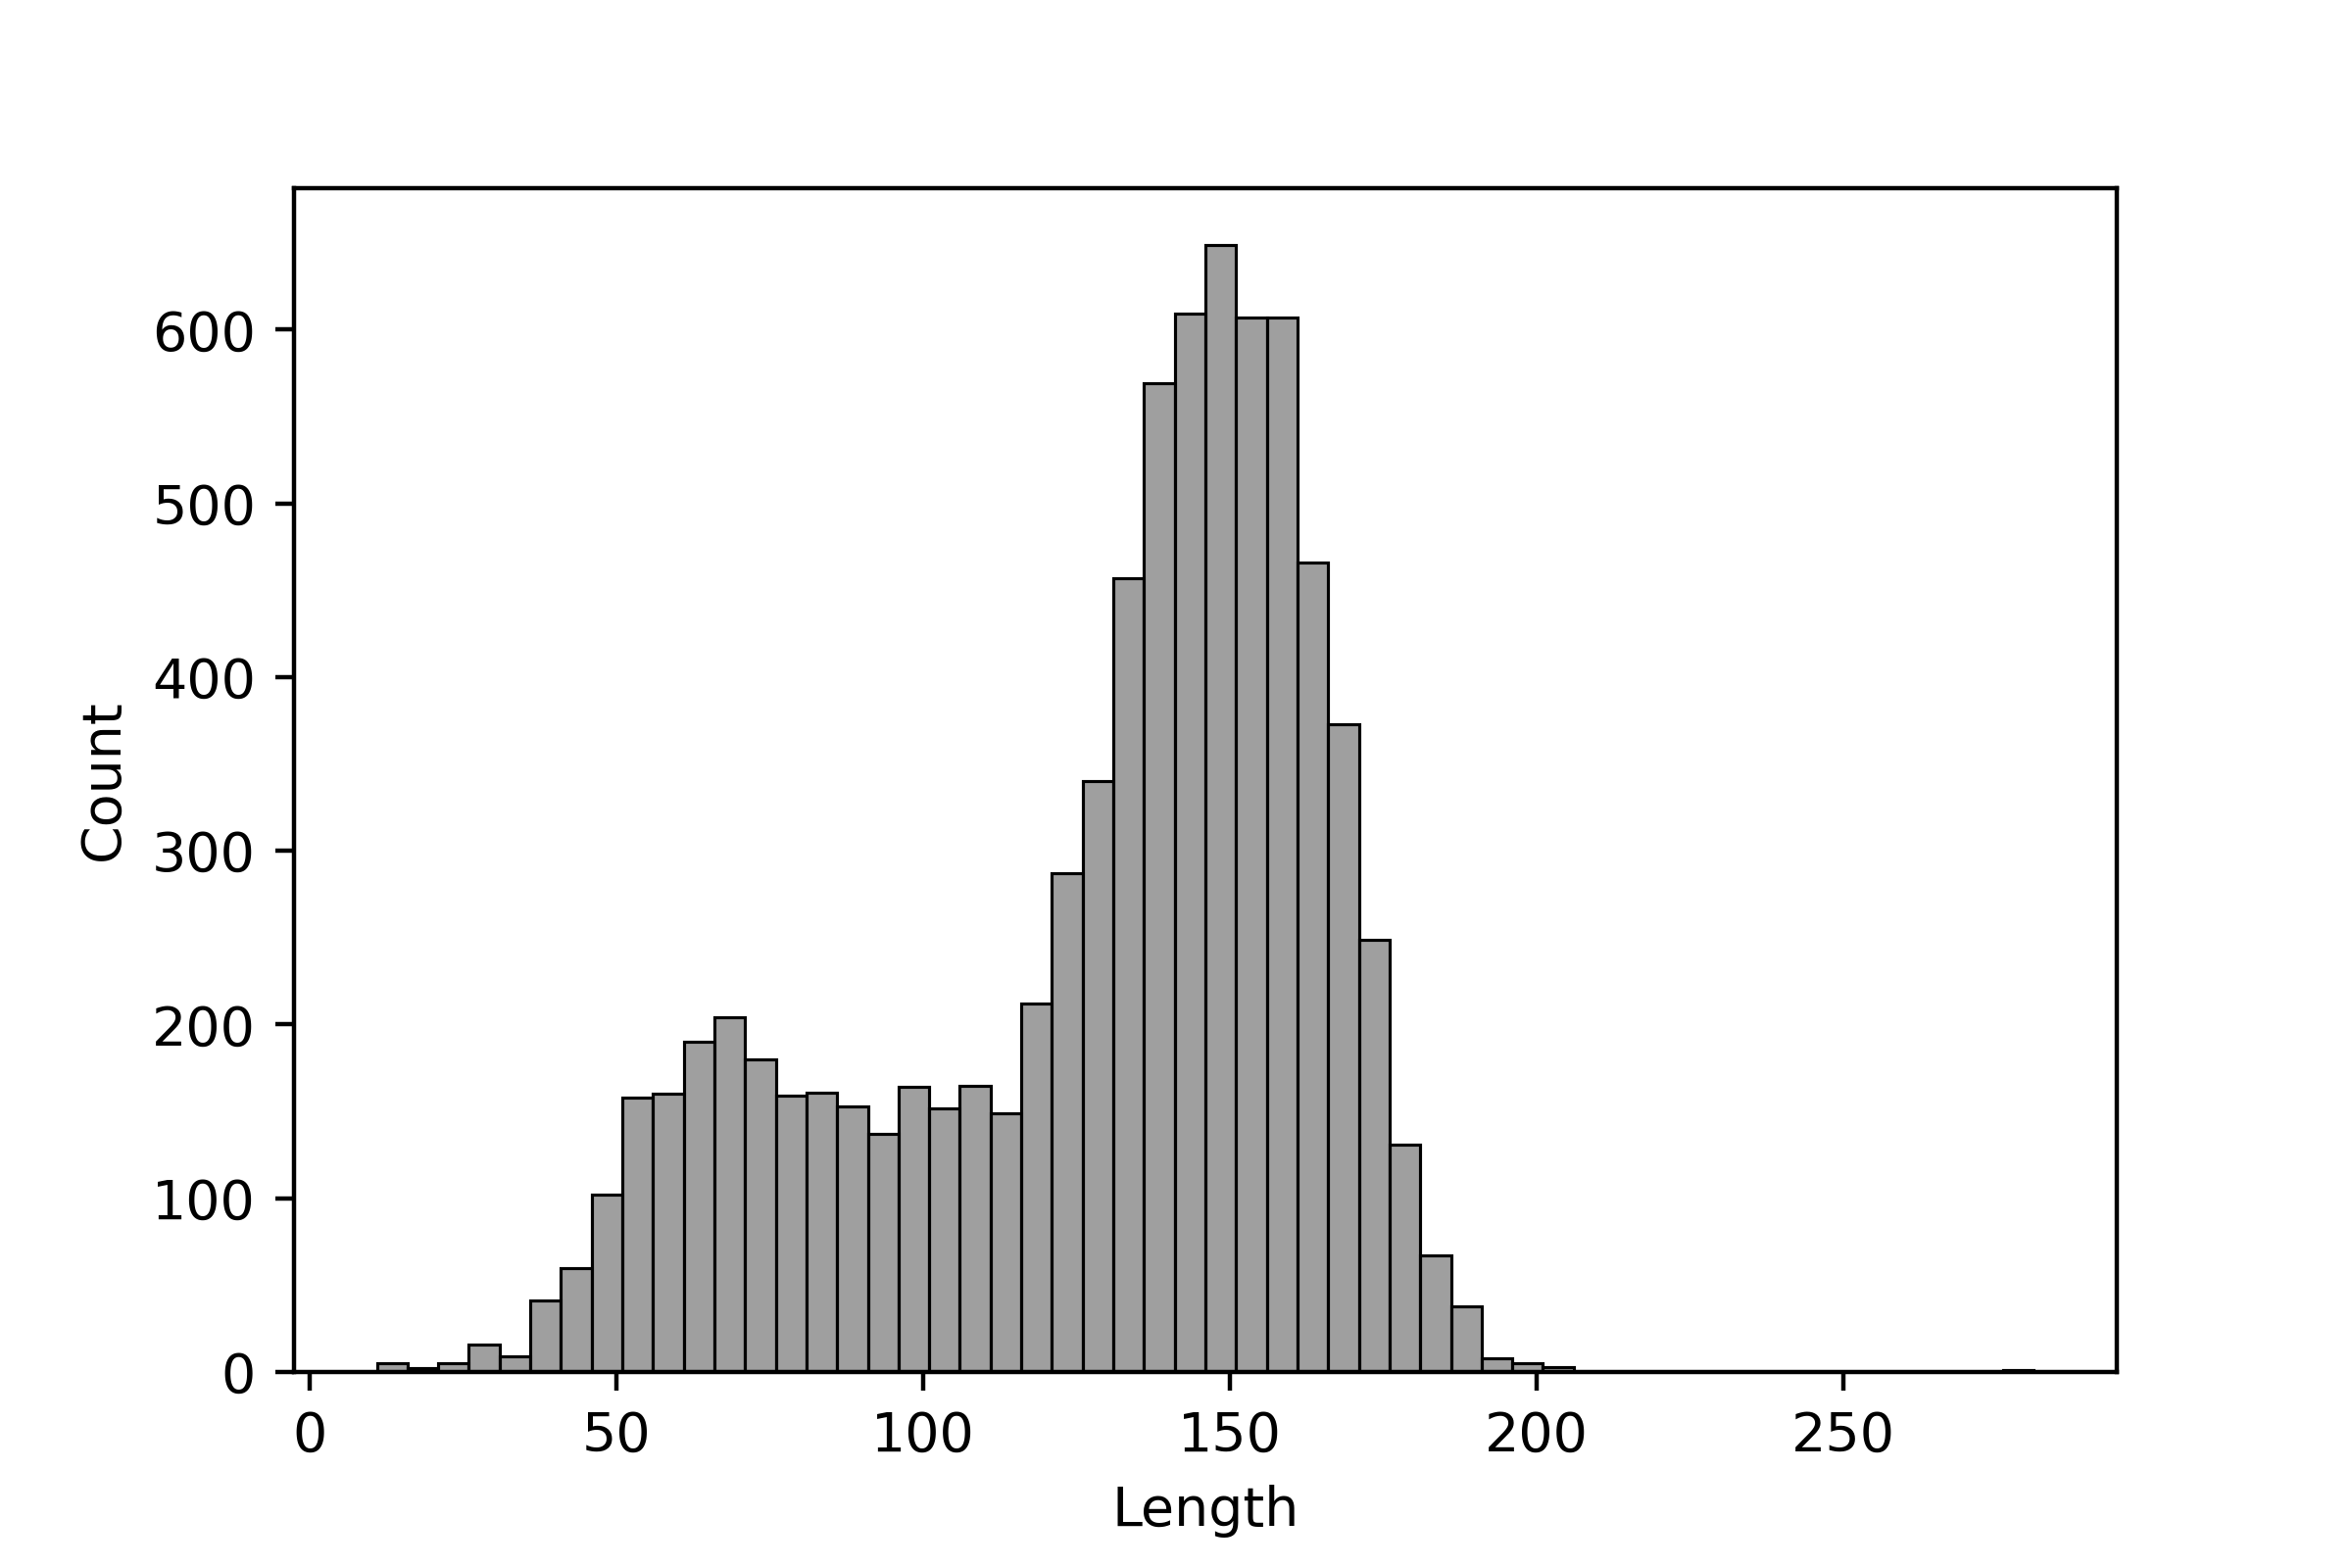
\includegraphics[width=.5\linewidth]{img/ImdbLengthdist.png}
%        \caption{IMDB Dataset.}{}
%          \label{fig:sub2}
%    \end{subfigure}
%\caption{Length Distribution of Fake news and IMDB Dataset.}{}
%\end{figure}

\section{Data Augmentation}
\label{section:dataaugmentation}

For creating the unlabeled augmented dataset, we have utilized three strategies :
\begin{enumerate}
\item  Synonym Augmentation
\item Context Based Augmentation
\item Back translation.
\end{enumerate}
While augmenting this dataset, there is a high chance that the information will be changed or completely opposite to the label of the original dataset. Therefore, once we augment the data, we will not use the label of the augmented data, so the augmented dataset will be unlabeled. For synonym changes, various python packages like text attack, nlpaug, and various basic python packages were used during experiments.\\
In addition, time and computation constraints have led us to choose the nlpaug data augmentation package \cite{ma_nlpaug_2022} to achieve all three augmentation strategies. We have augmented the dataset by removing the label columns from the train dataset and then randomly splitting it into three parts. The first part is for synonym augmentation, while the second part is for context based augmentation, and the last part is for back translation.\\
One more idea was to create unlabeled data using different attack recipes, which might provide better results under attack. However, the reason why attack recipes are not used is because the model is created with little or no understanding of how attacks work. \\
In the case of implementing a specific attack recipe to create unlabeled data,  robustness of the model will be enhanced for specific attack recipes, but overall evaluation of the model performance can be biased.\\
WordNet lexical English database \cite{miller_wordnet_1995} is used as a source of synonym augmentation, which includes word definitions, hyponyms, and semantic relationships. Same database is utilized for synonym replacement in this thesis. The maximum augmentation ($aug\_max$) parameter controls the level of augmentation. For IMDB and Covid-19  fake tweets datasets, it is set to 50 and 15, respectively. Another parameter called $iter$ is used to create two different copies of the synonym augmentation dataset. Example of generated synonym augmentation can be seen in table \ref{table:synaugment}.\\
\begin{table}[H]
    \centering
    \hspace*{-1.2em}
    \resizebox{0.8\textwidth}{!}{
        \begin{tabular}{|p{10cm}|p{10cm}|}
            \hline
           \hspace{30mm} \textbf{ Original Text}  &   \hspace{30mm} \textbf{	Augmented Text} \\
            \midrule
            \underline{look} how a true story  with a \underline{little} help of it s friends   a welldone and touching script  a good directing and a surprising great acting from a bunch of  no name  actors  \underline{especially} from the   yr old jodelle ferland  becomes a must seen movie  &
            \underline{search} how a true story with a \underline{lilliputian} help of it s friends a welldone and touching script a good directing and a surprising great acting from a bunch of no name actors \underline{peculiarly} from the yr old jodelle ferland becomes a must seen moving picture      \\
            \hline
            \underline{i} have to differ from the other comments \underline{posted}  amid sporadic funny moments  there are a \underline{lot} of actors trying too hard to be \underline{funny}  the strain shows  i watched this with \underline{two} friends on another friend s recommendation  none of us were \underline{thrilled}  &
            \underline{ace} have to \underline{disagree} from the other comments \underline{mail} amid sporadic rummy moments there are a \underline{circle} of actors trying too \underline{toilsome} to embody funny the strain shows i watched this with \underline{2} friends on another friend s recommendation none of us were thrill  \\
            \hline
        \end{tabular}
    }
    \caption[ Sample example of synonym based augmentation]{Sample example of synonym based augmentation from IMDB dataset. }
    \label{table:synaugment}
\end{table}
A context-based augmentation replaces the words in the sentence without changing the context. Generally, language models are used to accomplish this particular task, which is quite time- and memory-consuming. To perform this augmentation, DistilBERT language model is used.\\
\begin{table}[H]
    \centering
    \hspace*{-1.2em}
    \resizebox{.9\textwidth}{!}{
        \begin{tabular}{|p{10cm}|p{10cm}|}
            \hline
           \hspace{30mm} \textbf{ Original Text}  &   \hspace{30mm} \textbf{	Augmented Text} \\
            \midrule
          \underline{  i} loved this movie and will watch it again  original \underline{twist} to plot of \underline{man} vs man vs self  i think this is kurt russell s \underline{best} movie  his eyes \underline{conveyed} more than most actors words  perhaps there s hope for mankind \underline{in} spite of \underline{government} intervention  &
            \underline{listeners} loved this movie and will watch it again original \underline{note} to plot of \underline{beast} vs man vs self all think this is kurt russell \underline{bollywood} \underline{breakout} movie his eyes \underline{wander} more than most actors words perhaps our s hope for mankind \underline{knowing} spite of \underline{no} intervention \\
            \hline
        \end{tabular}
    }
    \caption[Sample example of context based augmentation]{ Sample example of context based augmentation from IMDB dataset. }
    \label{table:conaugment}
\end{table}
During back translation, sentences are converted in different languages and then translated back to the original language. In the same way, Marian's translation framework \cite{ma_nlpaug_2022}  is used, which is time and memory consuming. As part of our experiment, we are converting sentences into Romance language and back to English. We have used that model to perform this experiments. The Marian translation framework  is free, faster, and more efficient.\\
\begin{table}[H]
    \centering
    \hspace*{-1.2em}
    \resizebox{0.9\textwidth}{!}{
        \begin{tabular}{|p{10cm}|p{10cm}|}
            \hline
            \hspace{30mm} \textbf{ Original Text}  &   \hspace{30mm} \textbf{	Augmented Text} \\
            \midrule
           after \underline{seeing} the trailer for this movie and \underline{finding} out spike lee was directing  i was \underline{excited} to \underline{hear} about this event  i wasn t alive at the time \underline{ i didn t} \underline{live} in new york  so i expected more \underline{of} a history lesson \underline{than} \underline{anything}  \underline{what} i got was some interesting \underline{acting}  and about   minutes worth of film that actually had anything to do with the \underline{son of sam}  i guess the film wasn t about the \underline{son of sam } but it was a \underline{peek} into the summer of  label \underline{me disappointed  }   & 
            after \underline{watching} the trailer for this movie and \underline{knowing} that spike lee was directing, i was \underline{thrilled} to \underline{know} about this event that i wasn't alive at the time that i \underline{wasn't }\underline{living} in new york, so i expected more \underline{than} a history lesson \underline{that} \underline{nothing} \underline{that} i \underline{could} get was something interesting \underline{performing}  and about minutes of film that was really worth \underline{filming} that had something to do with \underline{sam's son}, i guess the movie wasn't about \underline{sam's son}, but it was a \underline{look} at the summer label \underline{i was disappointed} \\\\
            \hline
        \end{tabular}
    }
    \caption[ Sample example of back translation based augmentation]{ Sample example of back translation based augmentation from IMDB dataset. }
    \label{table:BTaugment}
\end{table}
Considering examples of all augmentation techniques, it is evident that  word perturbation are quite higher in back translation followed by context-based augmentation.

\section{Experiment Environment description}
\label{section: experimentenv}
The proposed experiment has been performed on two language models i.e. 1) $BERT_{Base}$ uncased version  and, 2) DistilBERT uncased version, model architecture is shown in figure \ref{fig:bertarch} and \ref{fig:DistilBERT} respectively. During this experiment baseline models will be referred as BERT and DistilBERT, and respective proposed model will be referred as MTBERT and MTDistilBERT. For training the models, google colab provided GPU has been utilized as shown in figure \ref{fig:nvidiagpu}. 
\subsection{Hyper parameter Details}
\label{subsection:hyperparameter}
To train the baseline model and proposed model, we used the hyper parameter values shown in table \ref{table:HyperparameterTable}. Exploring the performance of the model under different setting is not under the scope of this experiment. 
\begin{table}[H]
\centering
\begin{tabular}{ l c c }
\hline
Hyper parameter 		& \multicolumn{2}{c}{Used parameters in this work}\\
\hline
Optimizer 				& \multicolumn{2}{c}{Adam} \\
Learning rate 			& \multicolumn{2}{c}{ $2\epsilon -5$ } \\
Loss function 			& \multicolumn{2}{c}{Binary Cross Entropy}  \\
Epochs 				& \multicolumn{2}{c}{$3$} \\
Batch Size 			& \multicolumn{2}{c}{4 } \\
Loss Ratio 			&\multicolumn{2}{c}{0.5}\\
Alpha 			&\multicolumn{2}{c}{0.99}\\
Dropout  			& \multicolumn{2}{c}{0.2}  \\
Max length 			 & \multicolumn{2}{c}{100}  \\
\hline
\end{tabular}
\caption[Hyper-parameters Details]{Hyper-parameters Details}
\label{table:HyperparameterTable}
\end{table}
\section{Metrics}
\label{section:metrics}
During the experiment, generalization of the model is calculated by using accuracy of the target model on test samples, here referred as original accuracy i.e. the percentage of correct predictions over the entire sample set.
Next, we calculate robustness of the target models based on four different metrics: 
\begin{enumerate}
    \item Accuracy under attack 
    \item Attack success rate
    \item  Average number of queries
    \item Perturbation Score
\end{enumerate}
A target model's accuracy under attack is the percentage of correct predictions with respect to test samples, i.e. accuracy with respect to crafted test samples. Compared to the original accuracy, accuracy under attack can provide significant information about efficiency of the target model and attack recipes. Significant differences between these metrics indicate lower robustness against attack. A counter-part of accuracy under attack is the attack success rate, which indicates the effectiveness of attack recipes.\\
A metric other than accuracy is the average perturbed word in percentage, which is average number of words that need to change for successful attack. Higher word perturbation indicates less robustness, and this metric is also dependent on length of the text. \\
Furthermore, average number of queries i.e. number of times attacks recipes sends perturbed text sample input to target models for successful attacks. Higher number of queries is a sign robustness.\\
Finally, the perturbation score is a confidence score or a predicted probability of the target model under attack. Lower average perturbation score of only successful attacks can be a signal of better robustness. 

\section{Threat Model}
\label{section:threadmodel}
In this experiment, attack recipes are chosen based on level of knowledge, target, perturbation level, and assumptions. Considering most attacks are done under black box settings, the threat agent is only exposed to the target model output and test samples from the same corpus. Under this black box setting, a threat agent can only query the target model with perturbed inputs and get the corresponding confidence score or prediction. In addition, the threat agent is unaware of the model architecture, parameters, or training data. And, the agent can only query the target model with provided inputs. \\
As test samples are from the original corpus of the data, it is assumed that present test samples have been taken from different corpora. It is also assumed that attackers have access to similar baseline models. Because, similar tokenizers are used for tokenization in both while training and attacking, i.e. from the huggingface \cite{noauthor_hugging_nodate}  an open source python package for language models.\\
Evaluation of the model has performed for binary classification task, hence the attacks are mainly un-targeted but, because of binary classification it is assumed as targeted classification. And, only word level and multi-level which includes word and char level of word perturbation are considered. As, most of attacks are basically word level and character level hence, clear the intent of this selection.\\
The robustness of target models is evaluated against four attack recipes mentioned in \ref{section:attackrecipes}, hence it is assumed that threat agent has access to those attack recipes. And, the performance of model could be different if some other attack recipes are utilized.\\
 Furthermore, it is also assumed that the attack test samples are syntactically and semantically similar as per the claimed based on the attack recipes studies, hence, similarity metrics are not included in this experiment.\\
 The model is trained of mentioned settings  \ref{subsection:hyperparameter}, and the model can perform better or worse in different settings. In terms of the transferability, the experiment is conducted on two separate language models that differ in pre-training, it is expected that the approach would perform similarly if additional language models were used. 
%%%%%%%%%%%%%%%%%%%%%%%%%%%%%%%%%%%%%%%%%%%%%%%%%%%%%%%%%%%%%%%%CHAPTER RESULT ANALYSIS%%%%%%%%%%%%%%%%%%%%%%%%%%%%%%%%%%%%%%%%%%%%%%%%%%%%%%%%%%%%%%%%%%%%%%%%%%
\chapter{Experiment Result}
\label{chapter:result}
\section{Analysis of Result}
\label{section:resultanalysis}
The result presented in tables \ref{table:IMDBExpRes} and \ref{table:FakeNewsExpRes} demonstrates that MTBERT has outperformed all the other language models in almost all metrics. 
\begin{table}[H]
    \centering
    \hspace*{-0.8em}
    \resizebox{1.0\textwidth}{!}{
        \begin{tabular}{|c|c|c|c|c|c|c|}%{|l|l|r|r|r|r|r|}
            \toprule
            Attack Recipe&Model&  Ori. Acc.(\%)& Acc. und Attack(\%) &  Acc. Succ. Rate(\%) &   Avg. Pert. Word(\%) &   Avg. No. Queries  \\
            % Attack Recipe & Model &                     &                     &                      &                    &               \\
            \toprule
                 & BERT &                93.67 &                    33.93 &                  63.77 &                     \textbf{ 3.78} &           242.24 \\
            BAE  & DistilBERT &                92.85 &                    33.55 &                  63.87 &                      3.57 &           238.49 \\
                & MT BERT &                \textbf{94.13} &                    \textbf{56.45} &                 \textbf{ 40.03} &                      3.55 &           198.26 \\
                & MT DistilBERT &                93.17 &                    53.60 &                  42.47 &                      3.35 &           \textbf{284.94} \\
                \midrule
                 & BERT &                93.67 &                     0.60 &                  99.36 &                      3.97 &           749.33 \\
               PWWS & DistilBERT &                92.85 &                     1.70 &                  98.17 &                      4.07 &           750.24 \\
                & MT BERT &              \textbf{  94.13 }&                   \textbf{ 23.20} &                 \textbf{ 75.35} &                      \textbf{5.70} &          \textbf{ 890.84} \\
                & MT DistilBERT &                93.17 &                    17.82 &                  80.88 &                      5.38 &           866.78 \\
                \midrule
                 & BERT &                93.67 &                     2.30 &                  97.54 &                     22.04 &           235.27 \\
               TextBugger & DistilBERT &                92.85 &                     5.57 &                  93.94 &                     21.30 &           259.16 \\
                & MT BERT &                \textbf{94.13} &                    \textbf{35.13} &                 \textbf{ 62.68} &                     \textbf{28.57} &           \textbf{449.96} \\
                & MT DistilBERT &                93.17 &                    30.07 &                  67.73 &                     26.68 &           421.23 \\
                \midrule
                 & BERT &                93.67 &                     0.10 &                  99.89 &                      5.14 &           279.12 \\
                TextFooler & DistilBERT &                92.85 &                     1.07 &                  98.85 &                      5.07 &           278.73 \\
                & MT BERT &                \textbf{94.13} &                   \textbf{ 30.92}&                  \textbf{67.16} &                      \textbf{8.04} &           \textbf{720.77} \\
                & MT DistilBERT &                93.17 &                    25.48 &                  72.64 &                      7.54 &           613.91 \\
 \bottomrule
 \end{tabular}
    }
    \caption[Experiment Result of IMDB dataset]{IMDB dataset: MTBERT model has performed well overall followed by MTDistilBERT. }
    \label{table:IMDBExpRes}
\end{table}
\begin{table}[H]
    \hspace*{0.0em}
    \resizebox{1.0\textwidth}{!}{
        \begin{tabular}{|c|c|c|c|c|c|c|}%{|llrrrrr|}
            \toprule
            Attack Recipe& Model&   Ori. Acc.(\%)&Acc. und Attack(\%) &  Acc. Succ. Rate(\%) &   Avg. Pert. Word(\%) &   Avg. No. Queries  \\
            %Attack Recipe & Model &                     &                     &                      &                    &               \\
            \toprule
                 & BERT &                94.17 &                    67.53 &                  28.30 &                    \textbf{ 20.30} &            82.10 \\
               BAE & DistilBERT &                94.41 &                    67.66 &                  28.34 &                     18.99 &            79.12 \\
                & MT BERT &               \textbf{ 95.64} &                    \textbf{77.62} &                  \textbf{18.83} &                     16.57 &            \textbf{88.64 }\\
                & MT DistilBERT &                95.29 &                    74.04 &                  22.30 &                     19.46 &            86.47 \\
                \midrule
                 & BERT &                94.17 &                    24.68 &                  73.80 &                    \textbf{ 20.16 }&           215.04 \\
                PWWS & DistilBERT &                94.41 &                    25.68 &                  72.80 &                     19.18 &           210.62 \\
                & MT BERT &               \textbf{95.64} &                  \textbf{59.16} &                  \textbf{38.14} &                     17.93 &           \textbf{236.90} \\
                & MT DistilBERT &                95.29 &                    48.75 &                  48.84 &                     18.66 &           227.98 \\
                \midrule
                 & BERT &                94.17 &                    30.66 &                  66.69 &                    \textbf{ 24.87} &            82.55 \\
                TextBugger & DistilBERT &                94.41 &                    25.36 &                  73.14 &                     22.21 &            76.57 \\
                & MT BERT &               \textbf{ 95.64} &                    \textbf{65.61} &                  \textbf{31.39}&                     23.29 &           \textbf{114.25} \\
                & MT DistilBERT &                95.29 &                    53.99 &                  43.34 &                     24.54 &            96.14 \\
                \midrule
                 & BERT &                94.17 &                     7.62 &                  91.90 &                     22.48 &           180.55 \\
                TextFooler & DistilBERT &                94.41 &                     7.58 &                  91.98 &                     21.37 &           164.40 \\
                & MT BERT &                \textbf{95.64} &                   \textbf{ 54.05} &                  \textbf{43.48} &                     21.25 &           \textbf{282.66} \\
                & MT DistilBERT &                95.29 &                    40.90 &                  57.06 &                    \textbf{ 24.19} &           211.85 \\
            \bottomrule
        \end{tabular}
    }
    \caption[Experiment Result of Covid-19 fake tweets]{Covid-19 fake tweets Dataset: MTBERT model has performed well overall followed by MTDistilBERT.  }
    \label{table:FakeNewsExpRes}
\end{table}
The proposed approach models i.e. MTBERT and MTDistilBERT also performed better than the respective baseline models, i.e. BERT and DistilBERT.  As shown in figure \ref{fig:moaandauaimdb}, MT BERT model showed 0$\sim$2\% improvement in accuracy over the baseline model in both datasets and 20$\sim$30\% improvement in accuracy under attack. The proposed model also shown comparatively higher requirement for number of queries and word perturbations. Furthermore, the drop in accuracy is lowest in proposed approaches than baseline models.
%\begin{figure}[ht]
%    \begin{minipage}[b]{0.5\linewidth}
%        \centering
%        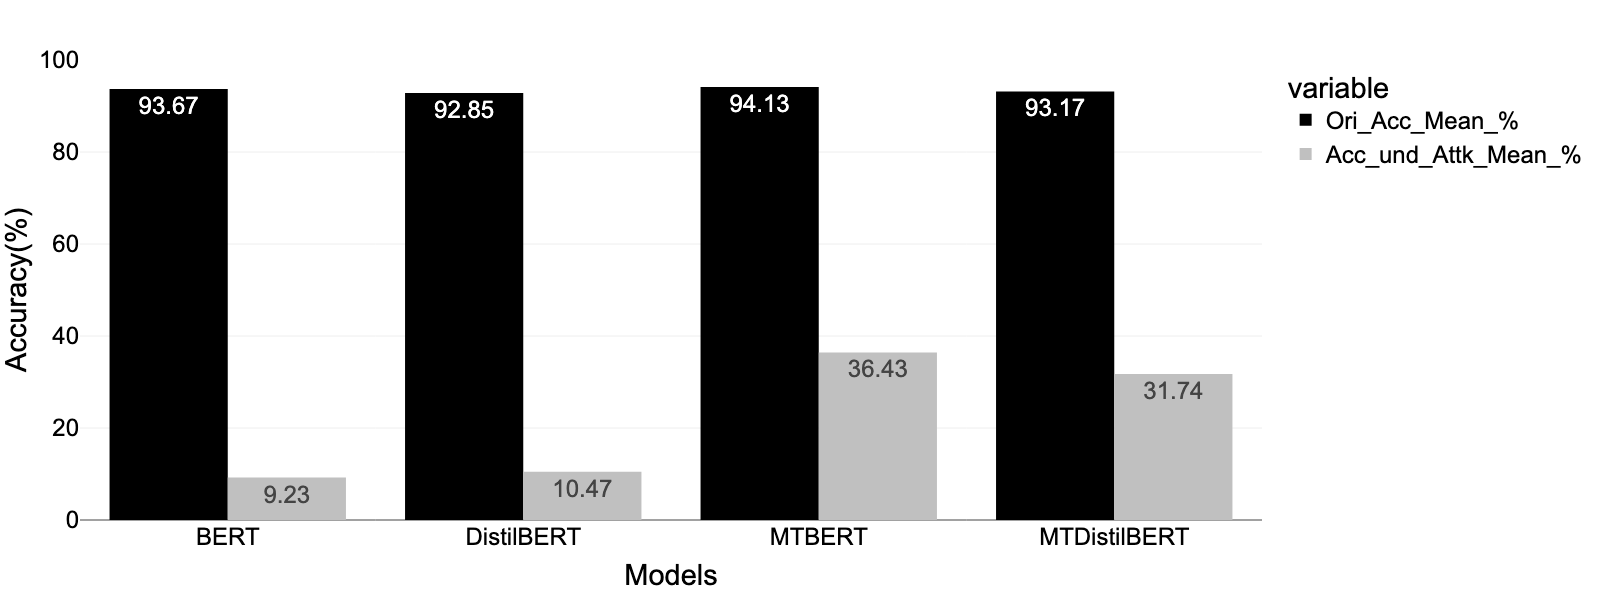
\includegraphics[width=\textwidth]{img/MOAandAUA_Imdb.png}
%%        \caption{IMDB Dataset: Original Accuracy and Accuracy under attack bar plot.}{}
%        \label{fig:imdboa}
%    \end{minipage}
%    \hspace{0.5cm}
%    \begin{minipage}[b]{0.5\linewidth}
%        \centering
%        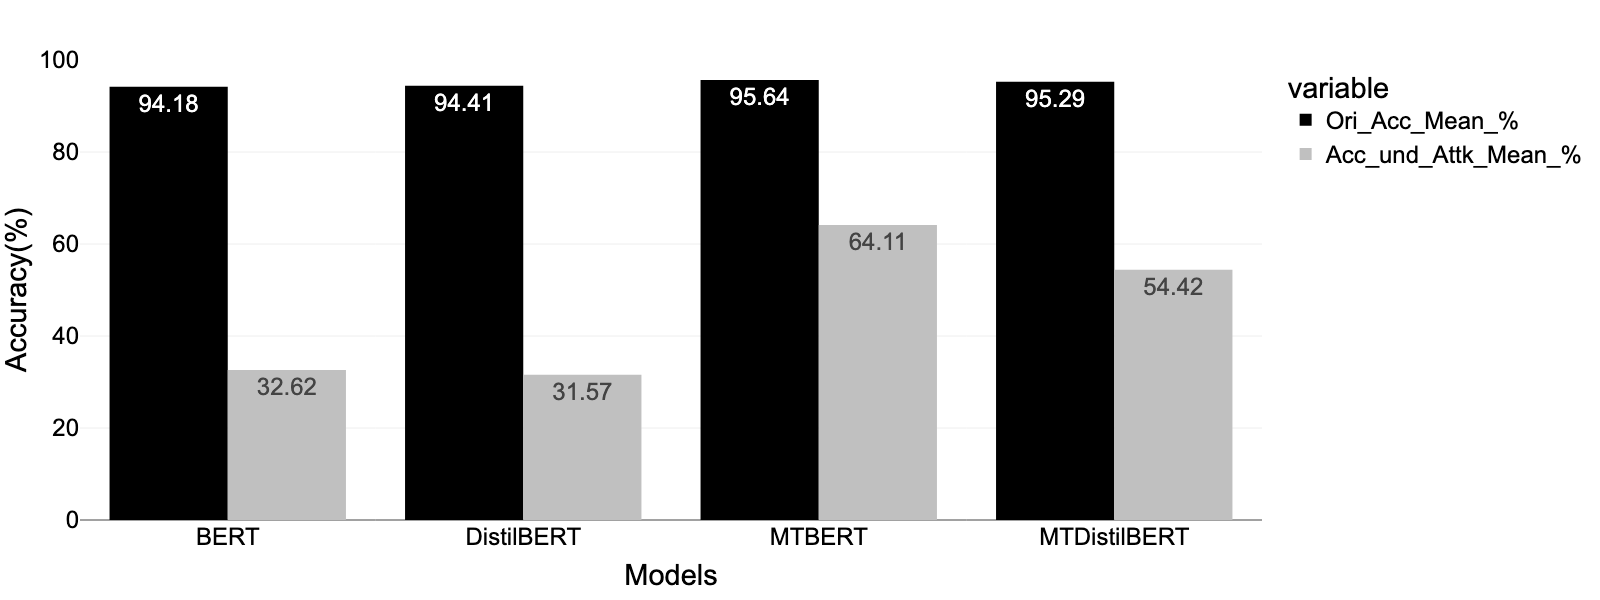
\includegraphics[width=\textwidth]{img/MOAandAUA_fknews}
%%        \caption{Covid-19 fake tweets dataset: }{}
%        \label{fig:fkoa}
%    \end{minipage}
%    \caption[Comparative bar plot of original accuracy and accuracy under attack]{\small Comparative bar plot of original accuracy and accuracy under attack in different dataset. MTBERT showed better performance in both metrics followed by MTDistilBERT. And, highest drop is seen in baseline models (BERT and DistilBERT).}
%    \label{fig:moaandauaimdb}
%\end{figure}

\begin{figure}[H]
    \centering
%    \hspace*{1.0em}
    \begin{subfigure}
            \centering
            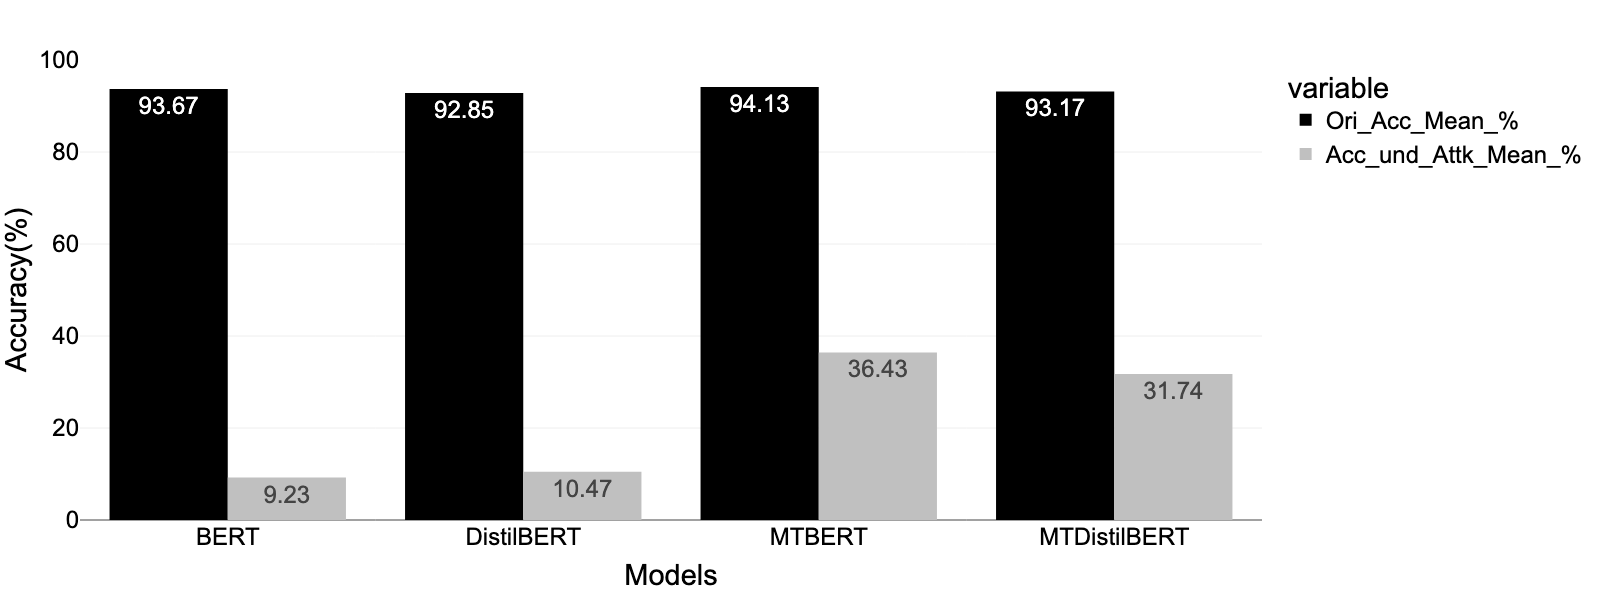
\includegraphics[width=.85\linewidth]{img/MOAandAUA_Imdb.png}
            \caption{IMDB Dataset.}{}
               \label{fig:}
        \end{subfigure}
%    \hspace*{1.8em}
    \begin{subfigure}
            \centering
            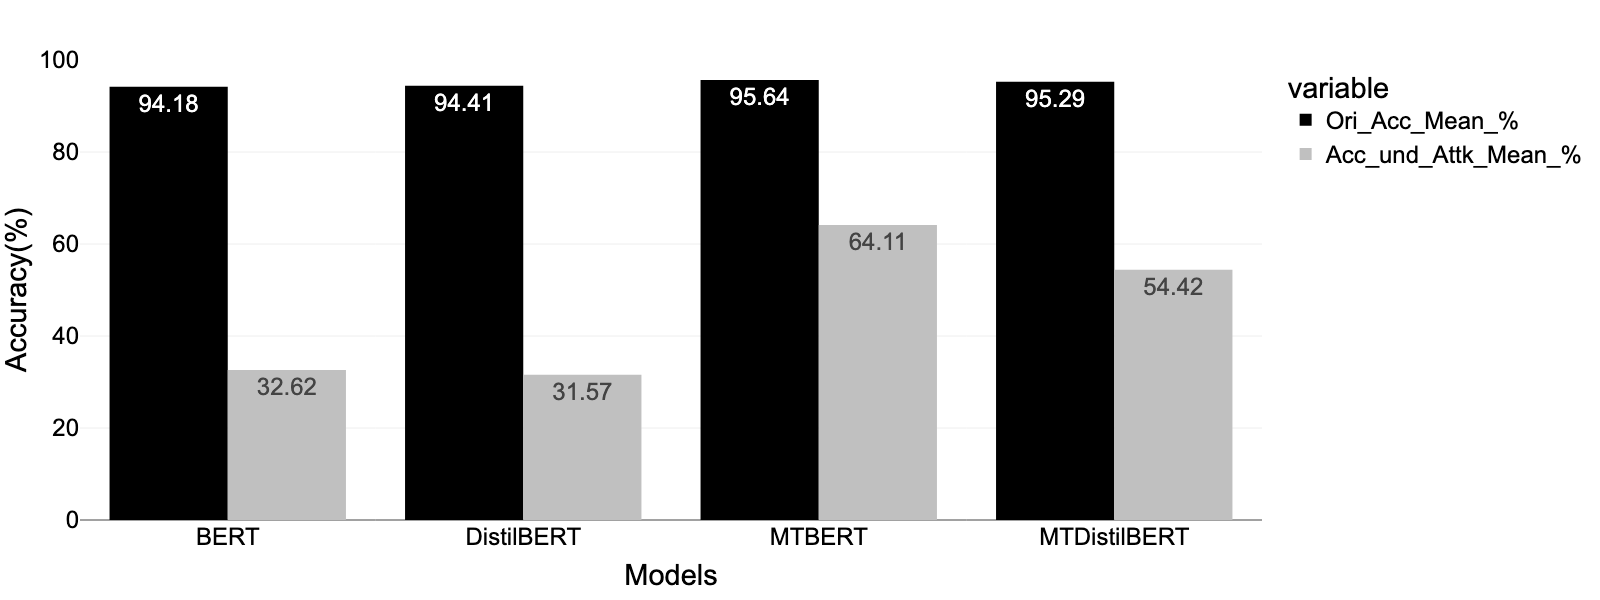
\includegraphics[width=.85\linewidth]{img/MOAandAUA_fknews}
            \caption{Covid-19 fake tweets dataset.}{}
              \label{fig:sub2}
        \end{subfigure}
 \caption[Comparative bar plot of original accuracy and accuracy under attack]{\small Comparative bar plot of original accuracy and accuracy under attack in different dataset. MTBERT showed better performance in both metrics followed by MTDistilBERT. And, highest drop is seen in baseline models (BERT and DistilBERT).}
  \label{fig:moaandauaimdb}
\end{figure}

In terms of queries, it is observed that overall MTBERT has high need for number queries to be attacked \ref{fig:avgnquebyattackrecipes}. As shown in box plot \ref{fig:numofqueriesdist}, the interquartile range of MTBERT and MTDistilBERT model is comparatively broader than any other models and has also shown incident crossing 2000 number of queries. \\

\begin{figure}[H]
	\centering
    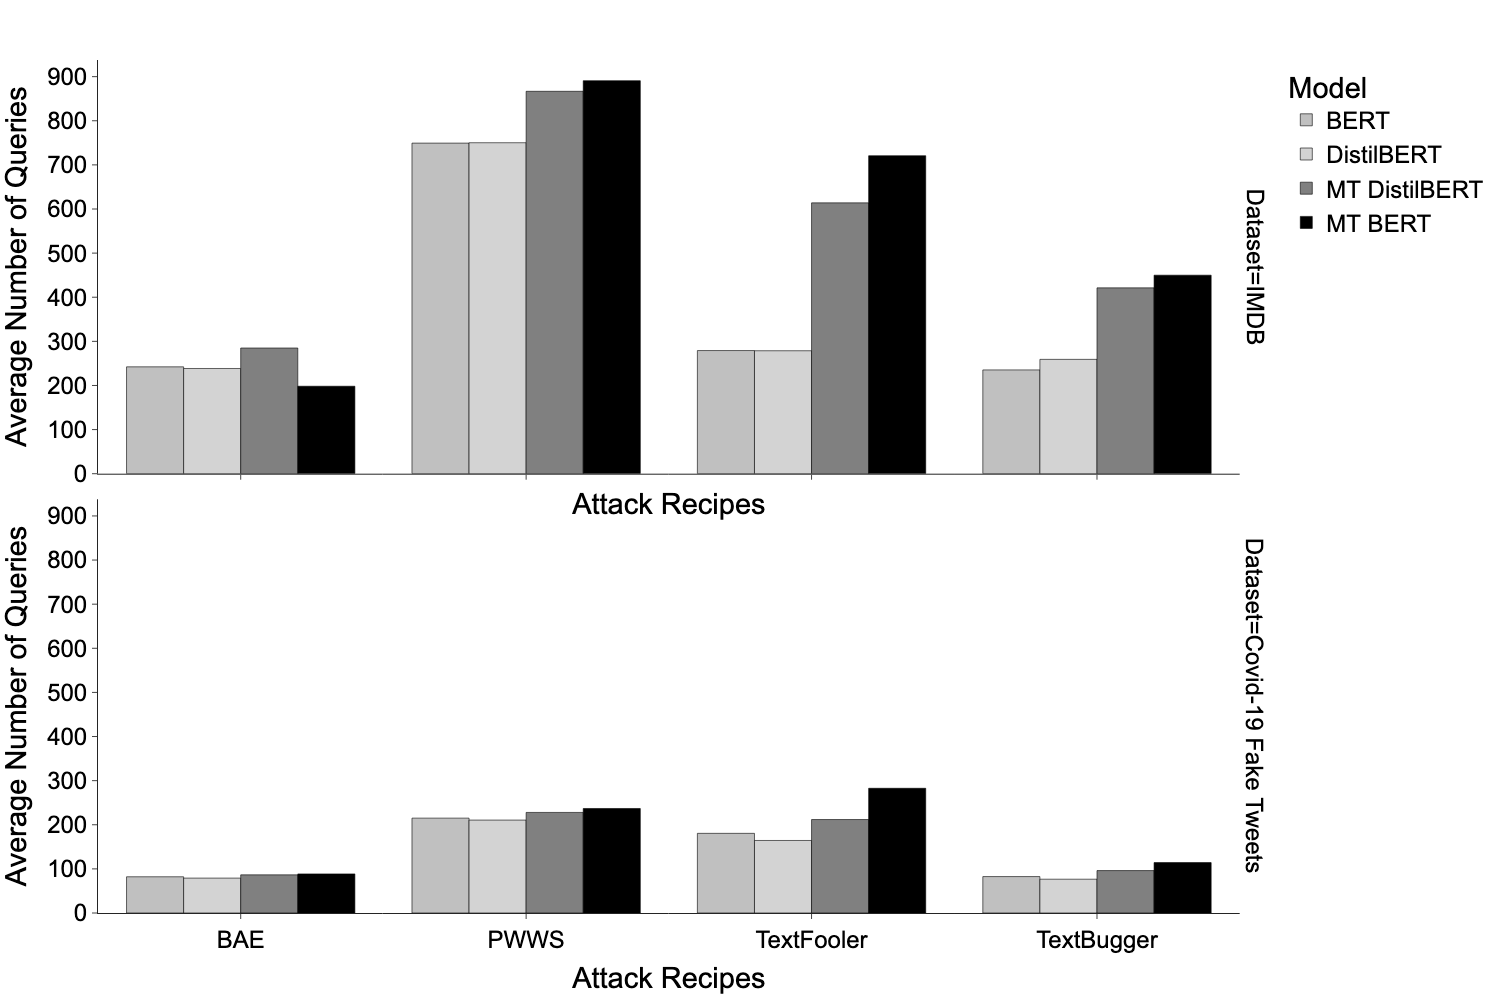
\includegraphics[width=.8\linewidth]{img/AvgNQuebyDataset}
	\caption[Bar plot of number of queries]{Bar plot of number of queries w.r.t dataset and attack recipes. PWWS has shown highest overall number of queries requirement followed by TextFooler.  And, dependencies w.r.t to text length can also be observed in this plot.}
	\label{fig:avgnquebyattackrecipes}
\end{figure}

\begin{figure}[H]
    \centering
    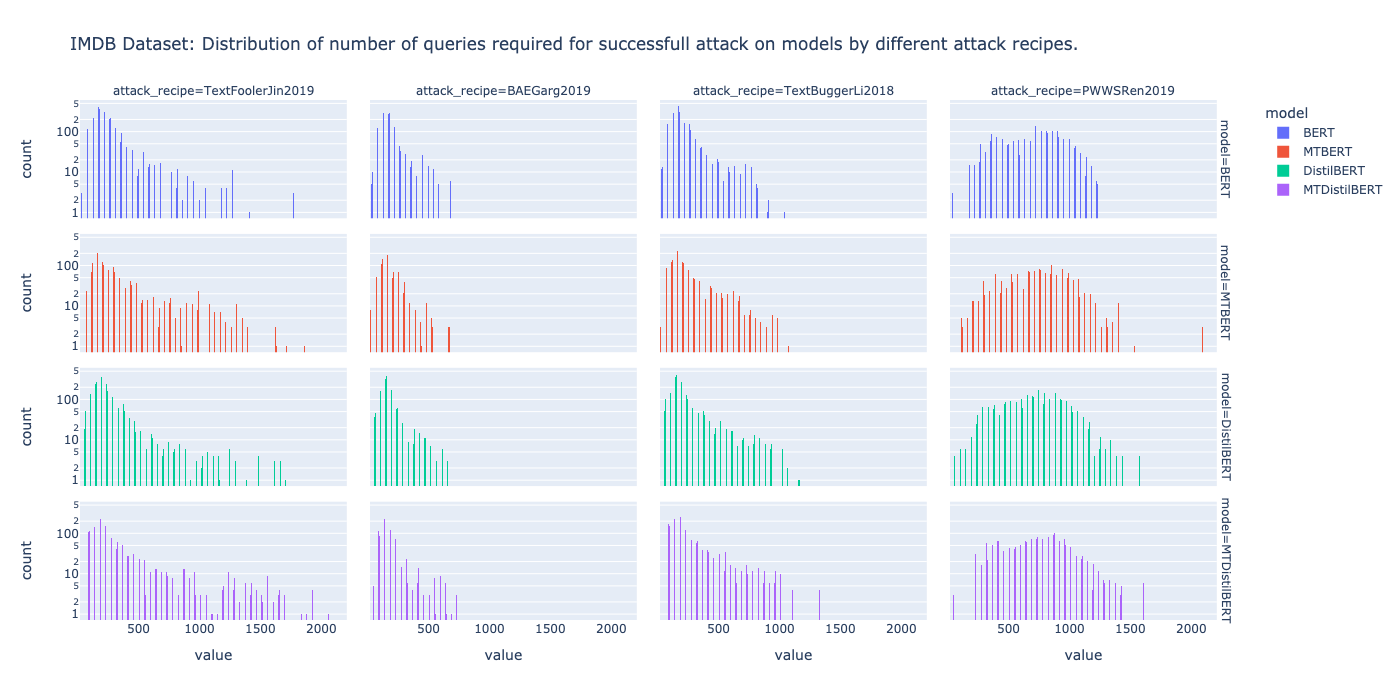
\includegraphics[width=0.7\linewidth]{img/NumQueriesDist_IMDB.png}
    \caption{Box-plot of number of queries.}{ The proposed model are comparatively more broader and showed greater values for outliers than baseline models. This particular box plot is based on IMDB dataset and only successful attacks are considered.}
    \label{fig:numofqueriesdist}
\end{figure}
If we compare the performances of attack recipes, BAE attacks have shown the lowest requirements for queries, followed by TextBugger, however, it is the least effective in attacking. PWWS requires a significantly higher number of queries followed by TextFooler and is also found to be more effective in attacks. Furthermore, both attack recipes are dependent on the text length, if we observe the considerable differences in queries as per dataset shown in figure \ref{fig:avgnquebyattackrecipes}. In TextFooler attack recipe, the difference between proposed and baseline queries also increases with respect to length of the text which shows its effectiveness depends on text length. \\
%%%
To understand the robustness of models with respect to word perturbation, the difference is less significant in between models as shown in figure \ref{fig:avgpertbyattackrecipes}. However, in the Covid-19 fake tweets dataset, the average word perturbation required by proposed models is higher, but, exactly opposite in IMDB dataset. It is quite clear that longer text requires comparatively lower word perturbation and also make sense. But, surprisingly TextBugger has shown the same perturbation rate and least affected by text length. However,  TextBugger requires a greater number of words perturbed than TextFooler. BAE required the lowest number of perturbations, followed by PWWS.
\begin{figure}[H]
    \centering
    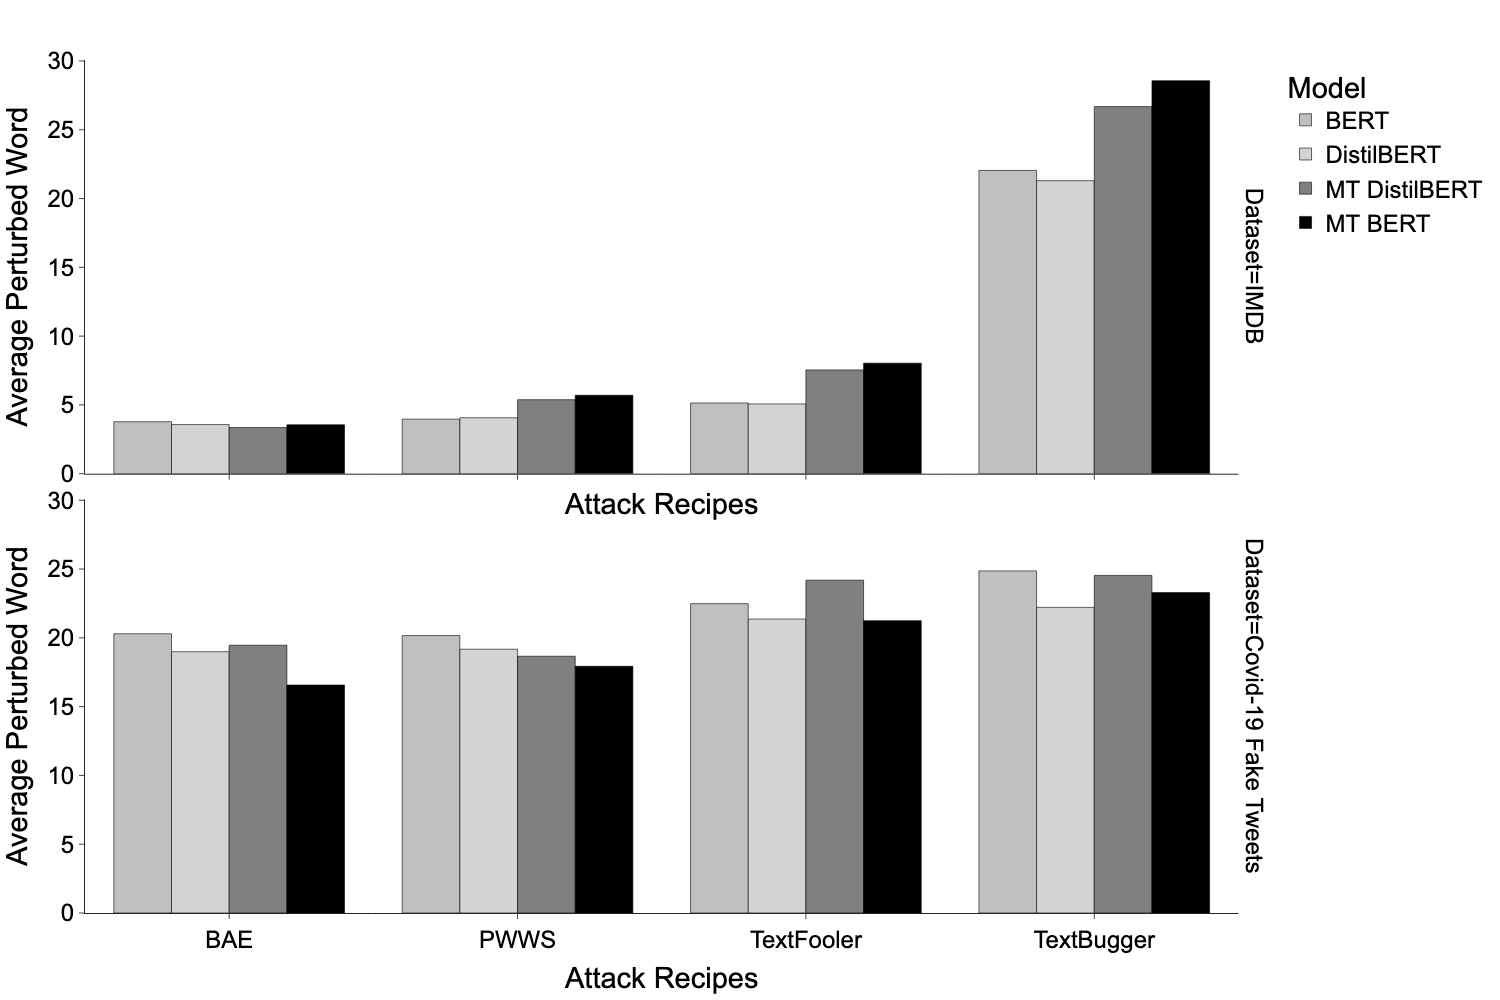
\includegraphics[width=0.8\linewidth]{img/AvgPertByDataset}
    \caption[Bar plot of Word perturbation]{Bar plot of Word perturbation as per datasets and attack recipes. TextBugger has shown highest word perturbation in both the datasets and also shown less difference between both dataset. However, BAE has lower word perturbation followed by PWWS attack recipe. Covid-19 fake tweets dataset has shown significantly higher word perturbation requirements.  }
    \label{fig:avgpertbyattackrecipes}
\end{figure}
Intuitively, while running the experiments we logged perturbation score that is predicted probability under attack in other term confidence score. To answer the question, how much proposed and baseline model let the attacker to change the confidence score of successful attacks. As shown in figure \ref{fig:pertscoredist}, huge improvement is being observed in proposed model  with respect to baseline model and the distribution of proposed model is comparatively more left shifted than baseline models. The proposed model does not let attack recipe go beyond a particular limit i.e. 0.70, however, baseline models are more uniform and shown less resilience.  The range of MT BERT model is 0.50 to 0.55, but for BERT model it is 0.50 to 0.66, which is a significant improvement in the model.

\begin{figure}[H]
    \centering
    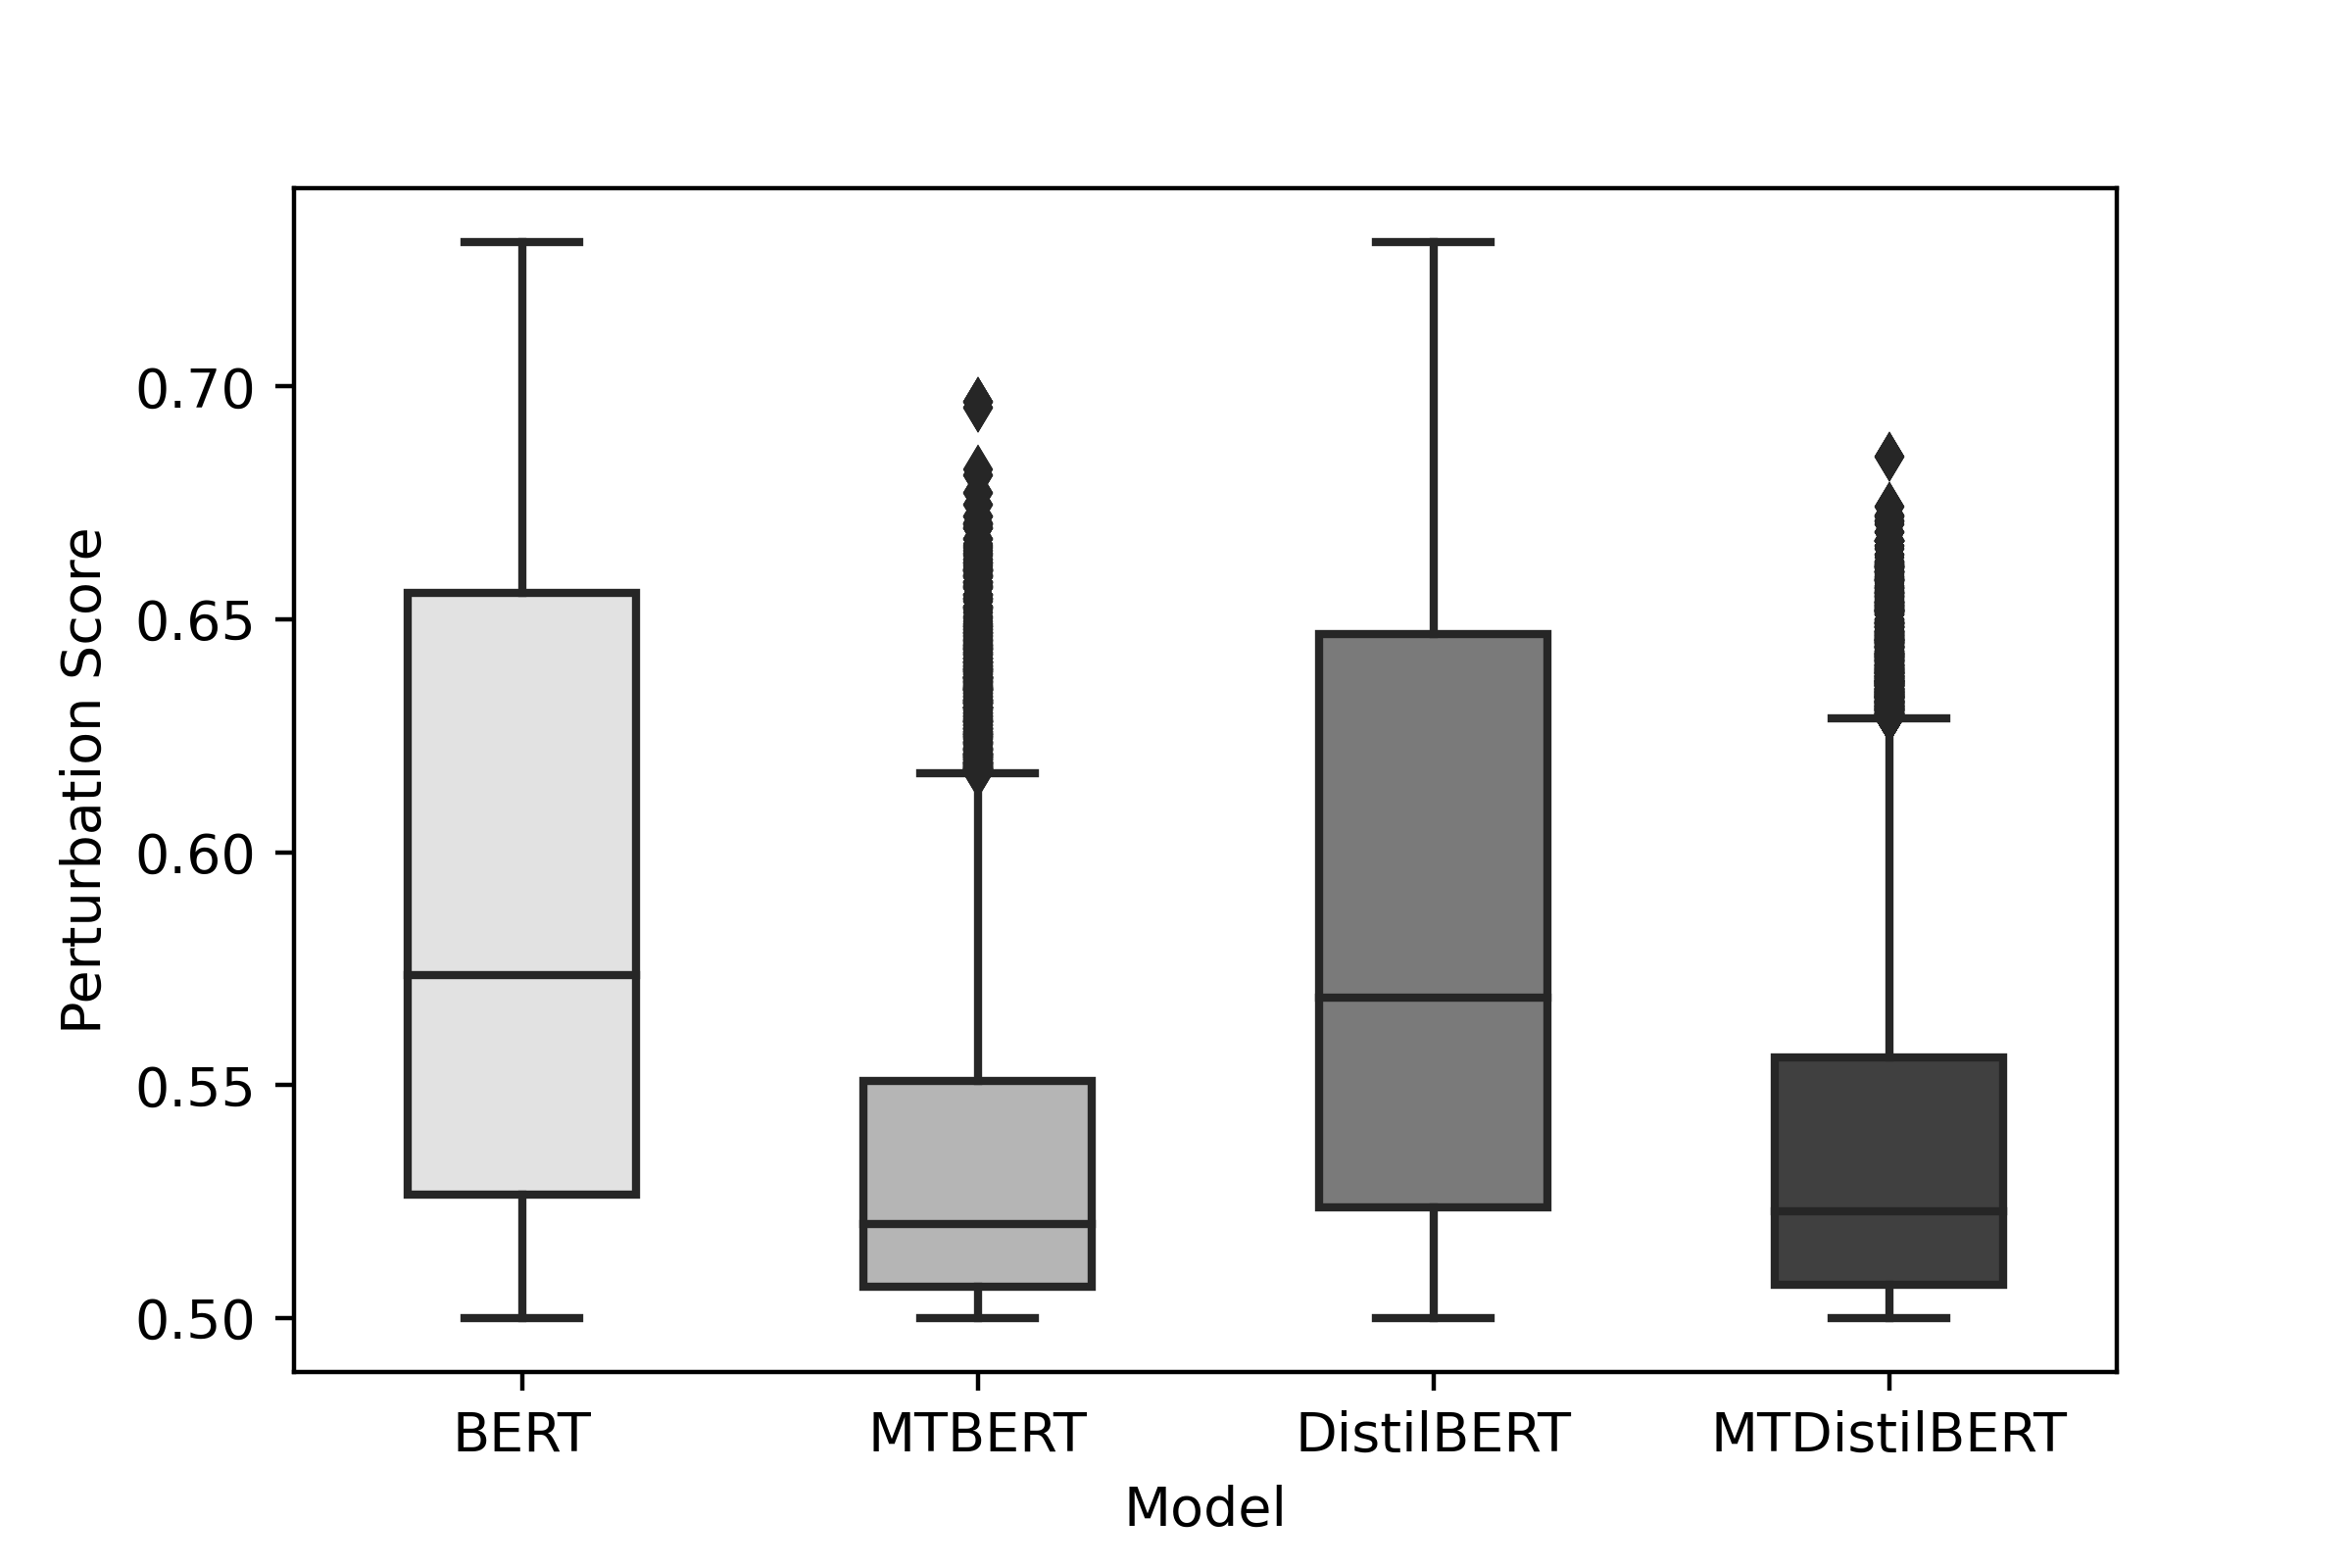
\includegraphics[width=.6\linewidth]{img/PertScoreDist}
    \caption[Box-plot of perturbation score]{\small Box-plot of perturbation score. MT BERT model has managed attacks confidence score in the leaner interquartile range and does not cross 0.70 in a single instance which is a significant improvement over BERT.}
    \label{fig:pertscoredist}
\end{figure}
 Overall, model fine-tuned using proposed approach has shown significant improvements over conventional way of fine-tuning and MT BERT has shown maximum robustness as compared to other models. According to the experiment, it is observed that knowledge distillation process of creating language posses more attack risk than original model. Furthermore, PWWS and TextFooler appeared to be more successful attacks recipes compared to other attack recipes. 

%\begin{figure}
%    \centering
%    \begin{minipage}{.5\textwidth}
%        \centering
%        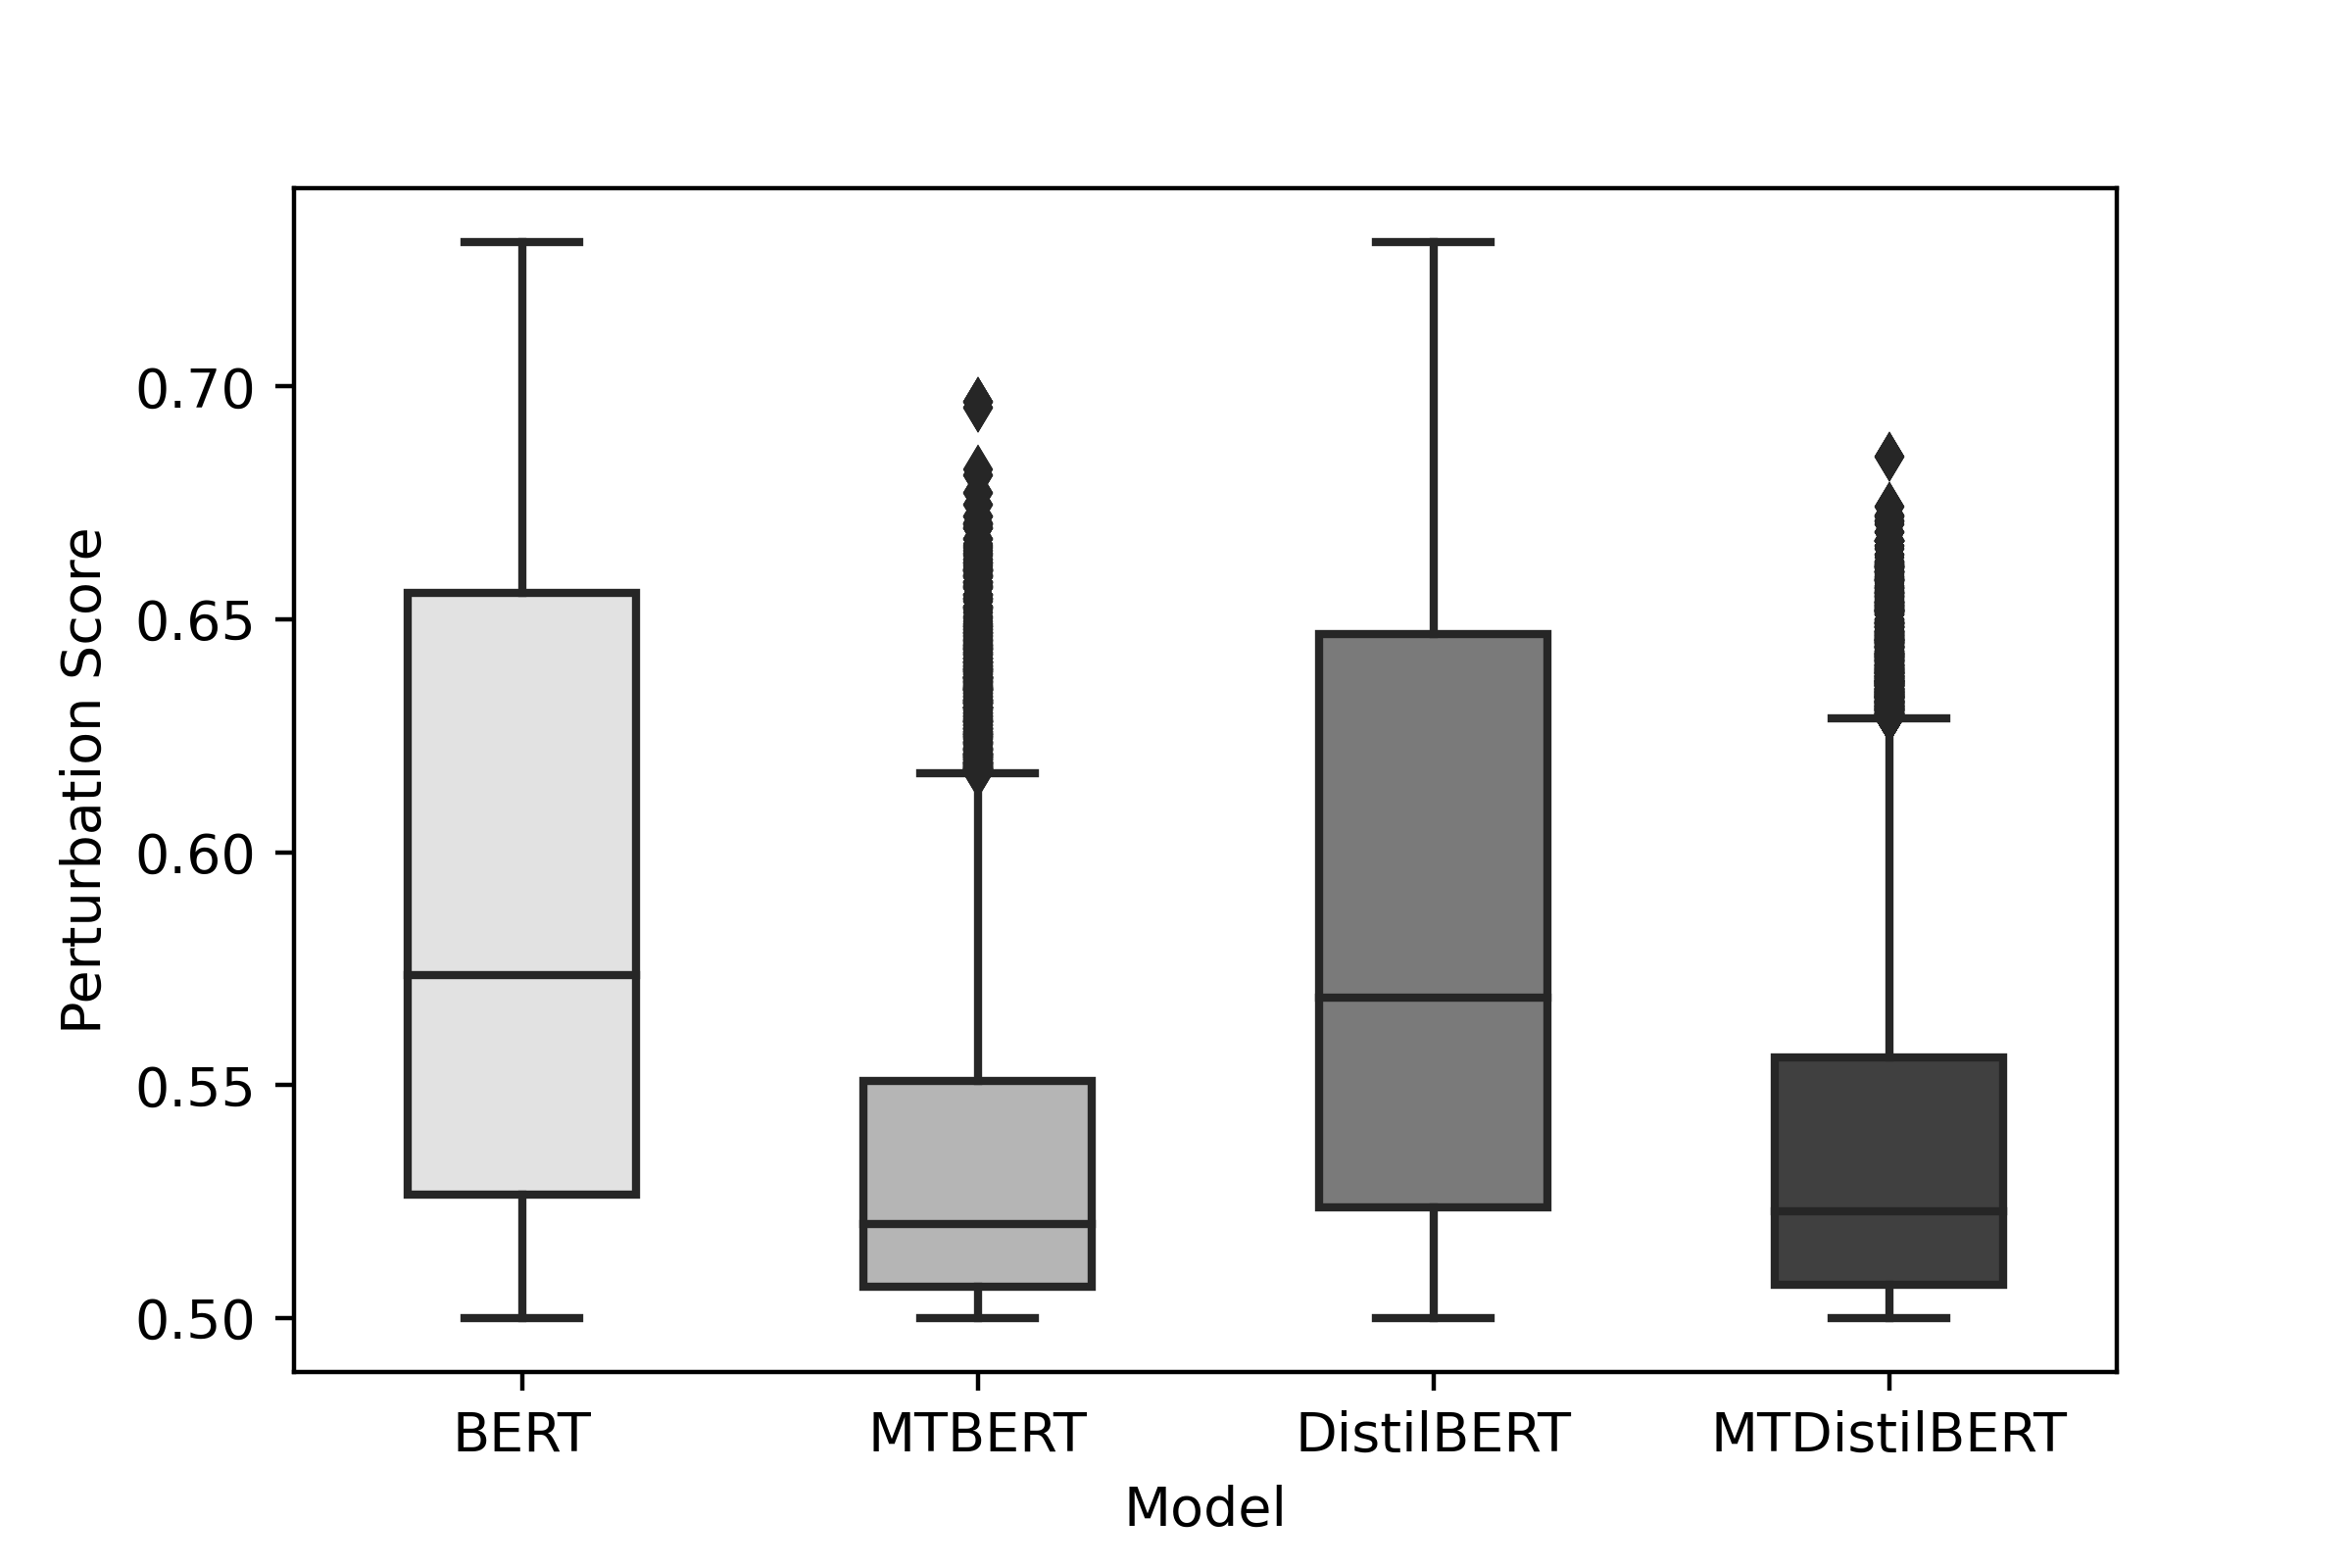
\includegraphics[width=.6\linewidth]{img/PertScoreDist.png}
%        \captionof{figure}{A figure}
%        \label{fig:test1}
%    \end{minipage}%
%    \begin{minipage}{.5\textwidth}
%        \centering
%        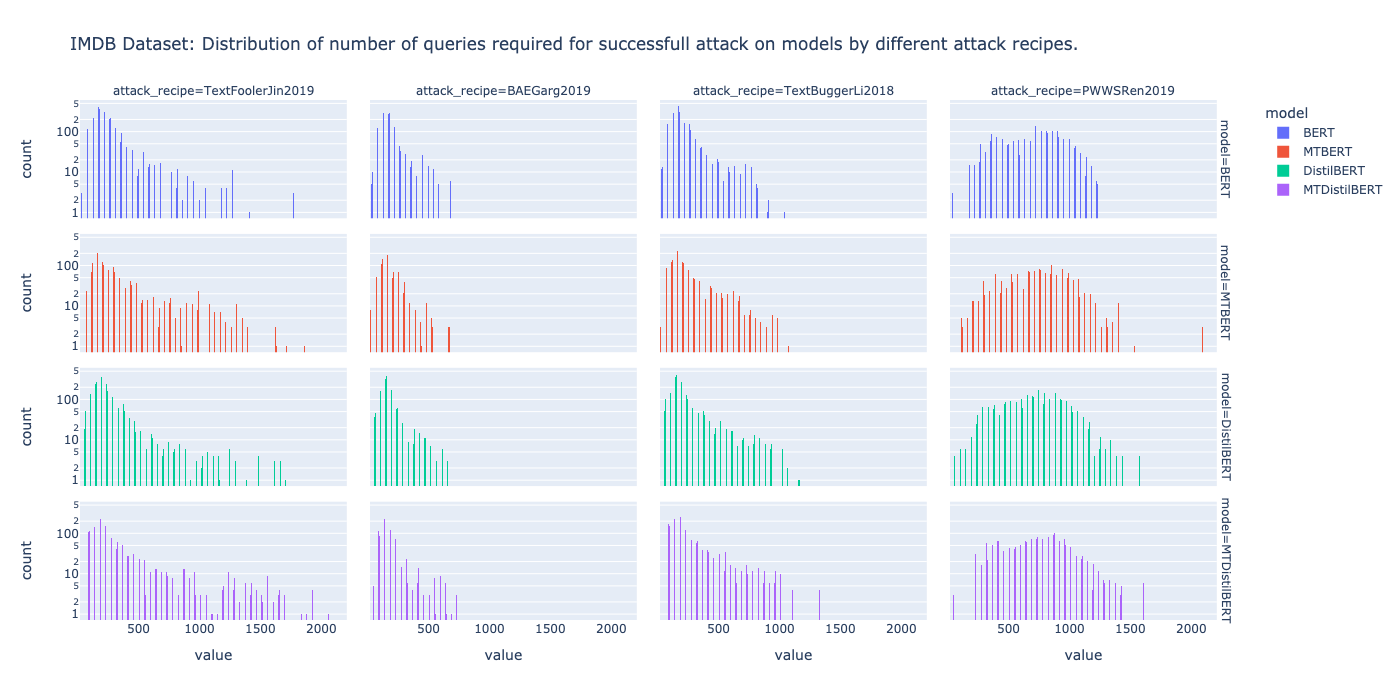
\includegraphics[width=.6\linewidth]{img/NumQueriesDist_IMDB.png}
%        \captionof{figure}{Another figure}
%        \label{fig:test2}
%    \end{minipage}
%\end{figure}

%\begin{table}[h!]
%    \centering
%    \hspace*{-0.7em}
%    \resizebox{1.0\textwidth}{!}{
%        \begin{tabular}{llrrrrrrrr}
%            \toprule
%            {} &         model &     count &  mean &  std &  min &  25\% &  50\% &  75\% &  max \\
%            \midrule
%            0 &          BERT & 38,507.00 &  0.59 & 0.07 & 0.50 & 0.53 & 0.57 & 0.66 & 0.73 \\
%            1 &    DistilBERT & 47,222.00 &  0.59 & 0.07 & 0.50 & 0.52 & 0.57 & 0.64 & 0.73 \\
%            2 &        MTBERT & 22,262.00 &  0.53 & 0.04 & 0.50 & 0.51 & 0.52 & 0.55 & 0.70 \\
%            3 &  MTDistilBERT & 32,012.00 &  0.54 & 0.04 & 0.50 & 0.51 & 0.52 & 0.56 & 0.67 \\
%            \bottomrule
%        \end{tabular}
%  }
%    \caption{Perturbation score table }{Perturbation score descriptive statistics of  successful attacks combining both dataset. Proposed model has shown significant improvement over baseline model. 
%        And, mostly in limited in range 0.53-0.70 and 75 \% of attacks score is under 0.55 a sign of robustness.}
%    \label{table:perturbationscore}
%\end{table}

\section{Discussing on Research Questions}
According to the results of the experiment and analysis, the baseline model outperformed other models and demonstrated high robustness. In comparison, the proposed technique has shown considerable gains in generalization as well as a much lower attack success rate. Furthermore, a higher word perturbation rate, fewer queries, and a lower perturbation score are all necessary.\\
This answers to the question that language models built with noisy data and includes a loss function called consistency loss during training can improve generalization and resilience. Also, if appropriate data augmentation procedures are implemented and the semi-supervised methodology of fine-tuning language models, i.e., can exhibit comparable outcomes in the text-domain.\\
The most typical explanation for the improvement is the inclusion of noisy data in training samples and the corresponding loss function, which plays a critical role in optimizing model weights. Also, protect the model against over-fitting, which prevents the model from gaining a deep understanding of the data. Furthermore, by integrating many new words as noise during training, models also learns a larger word representation. \\
Erik et al. \cite{englesson_consistency_2021} published a research that supports the recommended strategy. According to their findings, a model trained on noisy data has poorer consistency than one trained on clean data, and the consistency decreases even more as the noise ratio increases. Consistency regularization is the process of integrating a loss function during training in order to decrease consistency loss and generate a more robust model. The notion of consistency regularization is used in both gradient-based approaches \cite{miyato_adversarial_2017} and the suggested methodology.\\
Furthermore, the suggested method supports the findings of the Belinkov et al.\cite{belinkov_synthetic_2018} study, which claim that incorporating noisy data during training might improve the model's resilience. The experiment's transferability to other language models is partially demonstrated by the fact that it was conducted in two separate models, namely BERT and DistilBERT. Furthermore, this experiment also demonstrated that knowledge distillation process actually posses much severe security risks in contrast to adversarial attacks and robustness of the original model in not transferred during distillation.\\
This research also found that while current language models may have performed admirably in a variety of tasks, they are no different from other DNN models in terms of resilience. However, on a more positive note, the findings show that language models still have room for growth in terms of generalization and resilience.

\chapter{Limitation, Future Work and Conclusion}
\label{chapter:conclusion}

\section{Limitations}
\label{section:limitations}
Unlike image data where perturbation can be made imperceptible to humans, achieving even a similar level of imperceptibility is still a challenge in text domain due to its discrete nature. Most studies claimed to manage the same level of syntactic and semantic similarity of the original text, but in reality, the samples could be recognized by a human.\\
Attacks, data augmentation techniques, and semi-supervised training methodologies established in the image domain cannot be easily applied to the text domain, necessitating a separate effort and commitment to implement and evaluate them.\\
The suggested technique outperformed traditional models in the experiment; nonetheless, it cannot be said to be resistant to all forms of assaults. No defense plan can handle all forms of attacks since the nature of the attack is uncertain. Furthermore, incorporating the corresponding noisy data can only strengthen the robustness of the system against the assaults.\\
There are currently no common assessment criteria or frameworks for evaluating different research and strategy techniques in the text-domain, necessitating more investigation. In another case, recent studies have concentrated on improving model generalization rather than examining the robustness of such techniques.


\section{Future Work }
\label{section:futurework}
This approach can be evaluated using more recent state-of-the-art language models, and the work could also focus on the hypothesis that extreme pre-training of language models can hurt their robustness. And in another case, the effectiveness of individual augmentation techniques on robustness can be studied.\\
In the experiment, training data is used to create augmented prominent unlabeled data, however,  huge amounts of unlabeled data could be used instead and performance could be evaluated. In another case, including the adversarial samples generated by attack recipes during training can also be evaluated. \\
The quantitative comparison of gradient-based adversarial training and the proposed fine-tuning approach remains an open question. Moving forward, including both techniques toward robustness can also be evaluated in the future. \\
In another scenario, more research is needed to build a common robustness verification framework that can be used to compare various methodologies.
 
\section{Conclusion}
\label{section:conclusion}
The aim of this study was to do a quantitative comparison of the suggested semi-supervised strategy to fine-tuning language models in terms of generalization and resilience. Also, focus on improving the resilience of the language model. Observing the efficacy of significant unlabeled adversarial data, which can lead to improved resilience.\\
 In this experiment, various attack recipes such as PWWS, BAE, TextFooler, and TextBugger, data augmentation techniques such as word synonym, context augmentation, and back translation, and two language models such as BERT and DistilBert were utilized.\\
the results of the experiment revealed that the proposed strategy of fine-tuning improved initial accuracy by 0 $\sim$ 2\% and accuracy under assault by 20 $\sim$ 30\%. Furthermore, it demonstrated greater requirements in terms of word perturbation and number of queries, demonstrating its robustness against traditional fine-tuning methods. In terms of confidence score, the suggested technique is more robust to attacks, which is a substantial improvement in the model.\\
Furthermore, this research first highlighted that language models are sensitive to adversarial attacks and also, showed scope for development. The experiment also provides the direction of developing defenses against adversarial attacks, which can be examined in more detail.


%%%%%%%%%%%%%%%%%%%%%%%%%%%%%%%%%%%%%%%%%%%%%%%%%%%%%%%%%%%%%%%%%%%%CHAPTER REFERENCES%%%%%%%%%%%%%%%%%%%%%%%%%%%%%%%%%%%%%%%%%%%%%%%%%%%%%%%%%%%%%%%%%%%%%%%%%%%%%

%\chapter{References}


%\bibliographystyle{IEEEtran}
%\bibliography{./NLP_adversarial}
\printbibliography

\chapter{APPENDIX}
\label{chapter:appendix}
\begin{figure}[H]
    \centering
    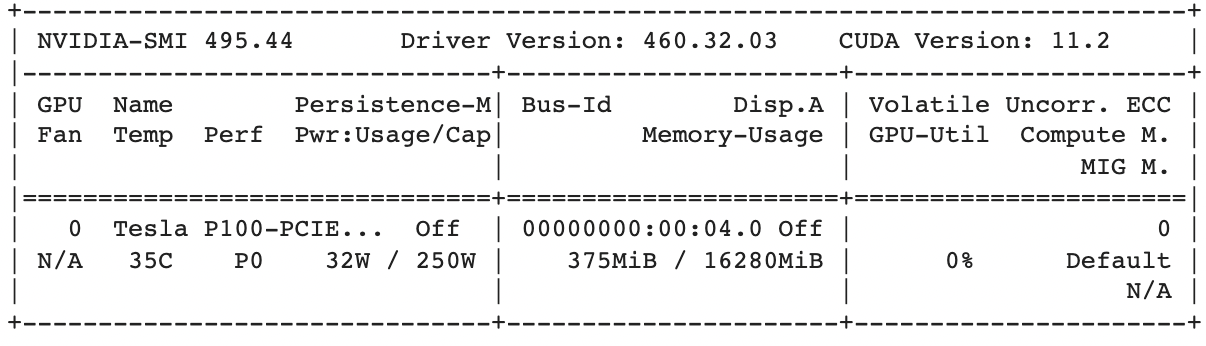
\includegraphics[width=0.9\linewidth]{img/nvidiagpu}
    \caption[Details of GPU]{GPU details}
    \label{fig:nvidiagpu}
\end{figure}
\begin{figure}[H]
    \centering
    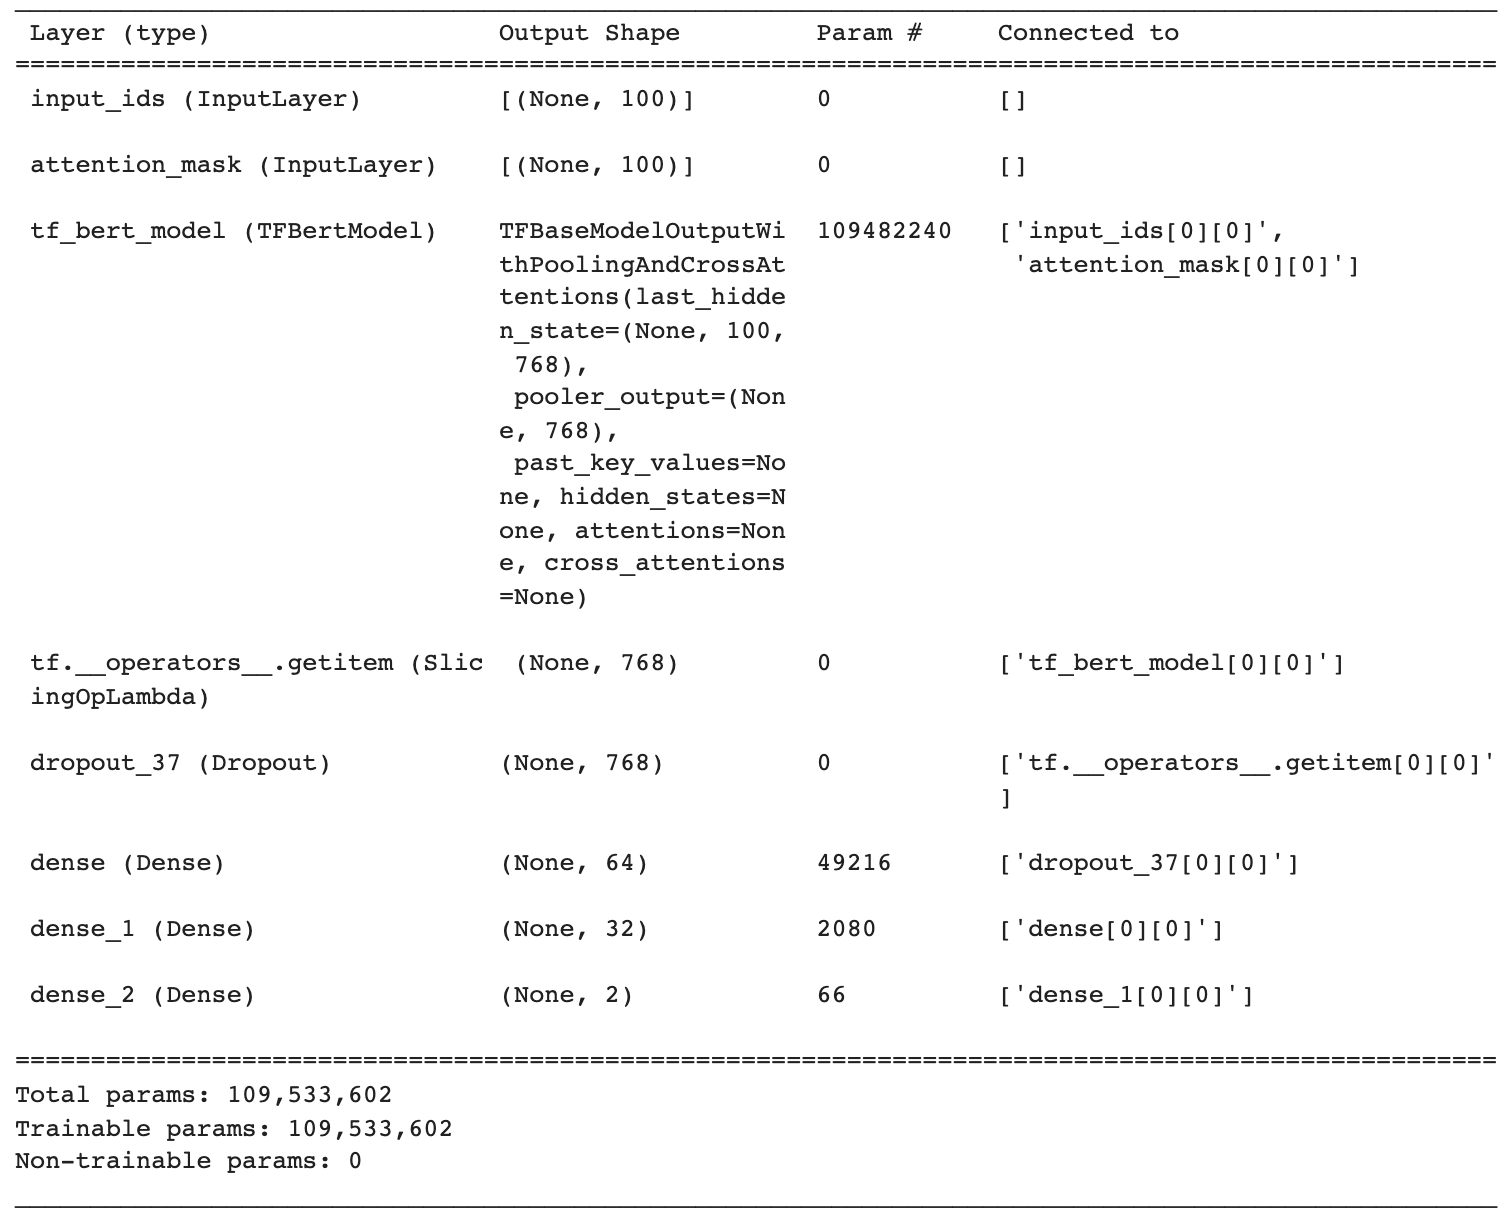
\includegraphics[width=0.8\linewidth]{img/bert_arch}
    \caption[ Layer diagram of BERT model used in the experiment]{Layer overview of BERT model used in the experiment}
    \label{fig:bertarch}
\end{figure}
\begin{figure}[H]
    \centering
    \includegraphics[width=0.8\linewidth]{img/DistilBERTarch}
    \caption[Layer diagram of DistilBERT model used in the experiment]{Layer diagram of DistilBERT model used in the experiment}
    \label{fig:distilbertarch}
\end{figure}


\end{document}


% \section{.tex Organization}

% This folder contains the following base structure:

% \begin{figure}[h!]
% \centering
% \begin{forest}
%   for tree={
%     font=\sffamily,
%     grow'=0,
%     child anchor=west, % orientation
%     parent anchor=south,
%     anchor=west,
%     calign=first,
%     draw,
%     top color=white, %  colors
%     bottom color=blue!20,
%     edge+=->,
%     edge path={ % edge configuration
%       \noexpand\path [draw, \forestoption{edge}]
%       (!u.south west) +(7.5pt,0) |- node[fill,inner sep=1.25pt] {} (.child anchor)\forestoption{edge label};
%     },
%     before typesetting nodes={
%       if n=1
%         {insert before={[,phantom]}}
%         {}
%     },
%     l sep'+=10pt, % distances
%     s sep=15pt,
%     node options={inner sep=8pt},
%     fit=band,
%     before computing xy={l=15pt},
%   }
% [FG\_Mauthe\_latex\_template
%   [template.tex \textbf{(main document)}]
%   [bibThesis.bib]
%   [inc
%     [Titlepage.tex \textbf{(update!)}, bottom color=red!20]
%     [Declaration.tex]
%     [Abstract.tex \textbf{(update later!)}]
%     [Glossary.tex \textbf{(optional)}]
%   ]
%   [img
%     [uni-logo.png]
%     [iwvi.jpg]
%   ]
% ]
% \end{forest}

% \caption{Folder structure with contents of this thesis template.}\label{fig:tree}
% \end{figure}


% \textbf{Important}:

% \begin{enumerate}
% \item \textit{template.tex} is the main document.
% \item \textit{bibThesis.bib} contains your future references.
% \item The \textit{inc} folder contains the necessary \textit{.tex} documents to complete your thesis.

% \item \textbf{Before you proceed and delete this text and the dummy chapters, please be sure to replace every important field in the title page! See the folder \textit{inc} and file \textit{titlepage.tex}.} Then, you are free to start writing your thesis!

% \begin{enumerate}
% 	\item Replace the title.
% 	\item Decide if bachelor or master.
% 	\item Put your course of studies.
% 	\item Put your name and matriculation number.
% 	\item Put month and year of the submission of your thesis. Keep this in mind in case of possible changes.
% 	\item Choose the second referee ("Zweitgutachter").
% 	\item If there's a third person (i.e. external), uncomment the respective line in the \textit{titlepage.tex} file and list him or her as well.
% \end{enumerate}

% \item The glossary is optional and it is not included by default.
% \item Images, tables and diagrams belong to the \textit{img} folder, although you are free to add more folders to organize your work. Always add the folder as a prefix if you include an image, for instance, \texttt{\textbackslash includegraphics[width=200pt]\{\underline{img}/iwvi.jpg\}}

% \end{enumerate}

% \section{Recommendations}

% Here, we list some tips and notes.

% \begin{itemize}
% \item Every diagram / table / figure has a caption describing it. Diagram legends must be \textbf{effortlessly} readable.
% \item Every symbol, specifically math symbols, used throughout the text are to be described and properly introduced.
% \item Use present tense whenever possible.
% \item If you prefer a serif font, simply comment at the very beginning of the document \\\texttt{ \textbackslash renewcommand\{\textbackslash familydefault\}\{\textbackslash sfdefault\}}.
% \item If you would like to write your thesis in German, comment \texttt{\textbackslash usepackage[english]\{babel\}} and uncomment \texttt{\textbackslash usepackage[ngerman]\{babel\}} (at the very beginning of the document). For "Umlaute" use, for instance, the formula \textbackslash"o to write an \"o.
% \item If your thesis contains a lot of abbreviations, you can include a glossary. Uncomment the line right below the table of contents in the \textit{.tex} document. In the folder \textit{inc} you find the \textit{glossary.tex} file.
% \item For an appendix, you uncomment the package \texttt{\textbackslash usepackage[toc,page]\{appendix\}} and the given exemplary lines at the end of this \textit{.tex} document. \footnote[2]{Make very sparse use of footnotes}
% \end{itemize}


%===%

% \chapter{Short \LaTeX\ Guide}

% This chapter contains a very short list of rudimentary \LaTeX\ commands with explanations.


% \section{Including Graphics}

% Here, you see an example to include graphics.

% \begin{figure}[h]
% 	\centering
% 	
\includegraphics[width=200pt]{img/iwvi.jpg}
% 	\caption[IWVI Symbol]{This picture serves as an example in this template. It is the symbol of our institute. Always include a meaningful caption below a figure or table which explains the figure or table almost by itself. The text in the brackets [] next to \texttt{\textbackslash caption} appears in the table of figures.}
% 	 \label{fig:picLabel}
% \end{figure}

% With the \texttt{\textbackslash label\{labelName\}} command you can define a label and point to the reference with \texttt{\textbackslash ref\{labelName\}} in your text. Here is figure \ref{fig:picLabel} for example.


%===%

% \section{Including Equations}

% You can add equations, enumerate and reference them using \texttt{\textbackslash eqref}, like for equation \eqref{eq:error}.

% \begin{equation}
% \label{eq:error}
% \dfrac{\partial L}{\partial w_l} = (a_l - y_i) \sigma'(z_l) a_{l-1}
% \end{equation}

% If an equation consists of several parts, you can use \texttt{subequations} to number them.

% \begin{subequations}
% \begin{align}
% \mathbf{H}_1 &= 3 + 3 \\
% \mathbf{H}_2 &= 4 + 4  \\
% \mathbf{\hat Y} &= 5 + 5
% \end{align}
% \end{subequations}


%===%

% \section{Including Tables}

% The description given in the square brackets next to the \texttt{\textbackslash caption} command of table \ref{table:exampleTable} should appear in the list of tables. Additionally, \texttt{ \textbackslash multicolumn} and \texttt{ \textbackslash multirow} enables the combination of columns or rows.

% \begin{table}[th]
% \centering
% \begin{tabular}{ l c c }
% \hline
% Hyperparameter 		& \multicolumn{2}{c}{Used parameters in this work}\\
% \hline
% Optimizer 				& \multicolumn{2}{c}{Adam} \\
% Learning rate 			& \multicolumn{2}{c}{ $0.01$ } \\
% Loss function 			& \multicolumn{2}{c}{sparse categorical cross entropy}  \\
% Epochs 				& \multicolumn{2}{c}{$400$} \\
% Batch size 			& \multicolumn{2}{c}{32 } \\
% Dropout value 			& \multicolumn{2}{c}{0.1}  \\
% \midrule
% Results obtained in \%	& First run		& Second run \\
% \hline
% Accuracy 				& 0.955 		& 0.9522 \\
% Precision				& 0.955	 	& 0.952  \\
% Recall 				& 0.955  		& 0.952 \\
% F1-Score 				& 0.955		& 0.952
% \end{tabular}
% \caption[Hyperparameters with test run results]{This dummy table shows several hyperparameters used in two experiments with results of several metrics. }
% \label{table:exampleTable}
% \end{table}


%===%

% \chapter{Citing and References}

% Important information. \textbf{Please refer to our introduction to scientific writing ("Einf\"uhrung in das wissenschaftliche Schreiben") for further information as well}.

% \section{In General}

% How to cite correctly:

% \begin{itemize}
% \item \textcolor{red}{wrong}: ...as the related work indicates. \cite{Rose} \cite{ISLR} \cite{cuDNN} (\texttt{\textbackslash cite\{Rose\} \textbackslash cite\{ISLR\} \textbackslash cite\{cuDNN\}})
% \item \textcolor{blue}{correct}: ...as the related work indicates. \cite{Rose, ISLR, cuDNN} (\texttt{\textbackslash cite\{Rose, ISLR, cuDNN\}})
% \end{itemize}

%  \textbf{Don't reference sources you haven't read and don't omit references crucial to understand parts of your thesis. Keep in mind that this may be considered \underline{plagiarism} and your thesis is evaluated with \textit{not passed}, e.g., 5.0.}

% \section{Types of References}

% Here you find a list of different types of reference, ordered by importance respectively \textit{scientific} quality.

% \begin{enumerate}
% \item Journal articles, conference papers (good quality)
% \item Books
% \item Reports, tech reports, work reports
% \item Magazines
% \item Internet sources (exception is arXiv) (below average quality)
% \end{enumerate}

% \section{Must-Have Attributes}

% There are several must-have attributes certain reference types should always contain.

% \subsection{Article}

% See \cite{Rose} for an example.

% \begin{itemize}
% \item Title
% \item Names of the authors
% \item Year of publication
% \item Journal or source
% \end{itemize}

% \subsection{Book}

% See \cite{ISLR} for an example.

% \begin{itemize}
% \item Title
% \item Names of the authors
% \item Year of publication
% \item Publisher / Issuer
% \item Location
% \item If applicable, mention the page or chapter of the source, for instance \cite[p. 1]{ISLR} (\texttt{\textbackslash cite[p. 1]\{ISLR\}})or \cite[Chapter 1]{ISLR}
% \end{itemize}

% \subsection{Internet Source}

% See \cite{cuDNN} for an example.

% \begin{itemize}
% \item Title
% \item Names of the authors
% \item URL
% \item "Last accessed " + date
% \item Not mandatory but advisable to take a screenshot of a page! Websites may change or disappear.
% \end{itemize}

% Good luck with your thesis!




% Appendices if needed. There might be other ways to achieve this, like putting a separate .tex file in the inc folder
% even though this option presented would be valid, too.
%\begin{appendices}
%\chapter{Some Additional Information }
%Sample appendices chapter.
%\end{appendices}

%